% !TEX root = ./thesis.tex

% DOC
\documentclass[openright,a4paper,12pt, twoside]{report}
\usepackage[
	includehead,
	hmargin={3.6cm, 2.6cm},
	vmargin={2.5cm,2.7cm},
	headsep=.8cm,
	footskip=1.2cm]{geometry}

% LINE SPACING
\usepackage{setspace}

% coloured frames
\usepackage{mdframed}
\mdfdefinestyle{todo}{
				leftmargin=5pt,
				linecolor=white,
				backgroundcolor=Red!10!White}
%
\newcommand{\todofr}[1]{
				\begin{mdframed}[style=todo]
					\vspace*{-.3cm}
					{\singlespacing\small#1}
					\vspace*{.1cm}
				\end{mdframed}}


% HEADERS
\usepackage{fancyhdr}
\setlength{\headheight}{15pt}
\fancyhf{} % clear the header and footers
\pagestyle{fancy}
\renewcommand{\chaptermark}[1]{\markboth{\thechapter. #1}{\thechapter. #1}}
\renewcommand{\sectionmark}[1]{\markright{\thesection. #1}}
\renewcommand{\headrulewidth}{0pt}
\fancyhead[LO]{\emph{\leftmark}}
\fancyhead[RE]{\emph{\rightmark}}
\fancyhead[RO,LE]{\emph{\thepage}}

% PART PAGE
\makeatletter
\renewcommand\part{%
  \if@openright
    \cleardoublepage
  \else
    \clearpage
  \fi
  \thispagestyle{empty}%   % Original »plain« replaced by »emptyx
  \null\vfil
  \secdef\@part\@spart}
\makeatother

% HYPERREF
\usepackage[colorlinks=true,
			linkcolor=TitleCol,
			citecolor=DarkGreen,
			urlcolor=TitleCol,
			linktocpage=true,
			pdfstartview=FitH]{hyperref}

% FONT
\usepackage[english]{babel}
\usepackage[utf8x]{inputenc}
\usepackage[T1]{fontenc}
\usepackage[default]{sourcesanspro}

%\usepackage[titles]{tocloft}
%\renewcommand{\cftchapfont}{\large\sc}

% COLORS
\usepackage[usenames,dvipsnames,svgnames]{xcolor}

\definecolor{TitleCol}{HTML}{28316C} % sections, ...
\definecolor{EnvCol}{HTML}  {28316C} % theorem, ...
\definecolor{CapCol}{HTML}  {28316C} % fig, ...

% CAPTIONS
\usepackage[width=.8\textwidth,					% caption width
			labelfont={bf,sf,color=CapCol},		% caption style
			font={footnotesize},
			format={hang},
			textfont={it}]{caption}

% CHAP STYLE
\usepackage{titlesec}
\makeatletter 			% section & subsection number in margin
	\def\@seccntformat#1{
		\protect\makebox[0pt][r]{
			\csname the#1\endcsname\quad
			}
		}
\makeatother

\titleformat*{\section}{
	\Large\bfseries\selectfont\color{TitleCol}}
\titleformat*{\subsection}{
    \large\bfseries\selectfont\color{TitleCol}}
\titleformat*{\subsubsection}{
    \small\bfseries\selectfont\color{TitleCol}}

% BIBLIOGRAPHY
\usepackage[authoryear,sort]{natbib}

% TIKZ
\usepackage{tikz}
\usetikzlibrary{arrows,shapes}

% MATHS
\usepackage{amsmath}
\usepackage{amssymb}
\usepackage{amsthm}

\numberwithin{equation}{chapter}

% ALGORITHMS
\usepackage{algorithm}
\usepackage{algpseudocode}
\usepackage{algorithmicx}
% !TEX root = ./thesis.tex

%
% <D.1> Text
%
\newcommand{\begen} 		{\begin{enumerate}}
\newcommand{\stopen} 		{\end{enumerate}}
\newcommand{\noi}			{\noindent}
\newcommand{\fig}		[1] {\hyperref[#1]{figure \ref*{#1}}}
\newcommand{\nn}          	{\nonumber}
\renewcommand{\tt}		[1]	{\texttt{#1}}
\newcommand{\blue}		[1]	{\textcolor{blue}{#1}}
\newcommand{\dblue}		[1]	{\textcolor{Blue!70!NavyBlue}{#1}}
\newcommand{\blueit}	[1]	{\blue{\emph{#1}}}
\newcommand{\idblue}	[1]	{\dblue{\emph{#1}}}
\newcommand{\ddblue}	[1]	{\dblue{\textbf{#1}}}
\newcommand{\grayit}	[1]	{\gray{\emph{#1}}}
\newcommand{\dgray}		[1]	{\textcolor{Gray!80!Black}{#1}}
\newcommand{\idgray}	[1]	{\dgray{\emph{#1}}}
\newcommand{\dgreen}	[1]	{\textcolor{Black!40!OliveGreen}{#1}}
\newcommand{\dorange}	[1]	{\textcolor{Orange!40!Sienna}{#1}}
\newcommand{\red}		[1]	{\textcolor{red}{#1}}
\newcommand{\dred}		[1]	{\textcolor{BrickRed!60!Red}{#1}}
\newcommand{\idred} 	[1] {\dred{\emph{#1}}}
\newcommand{\clarify}	    {\dred{\textbf{\#\#\#\#}}\xspace}
\newcommand{\gray}		[1]	{\textcolor{Gray}{#1}}
\newcommand{\green}		[1]	{\textcolor{DarkGreen}{#1}}
\newcommand{\magenta}	[1]	{\textcolor{magenta}{#1}}
\newcommand{\orange}	[1]	{\textcolor{orange}{#1}}
\newcommand{\begar}			{\begin{itemize}[$\dblue{\rightarrow}$]\itsep{0}}
\newcommand{\stopar}		{\end{itemize}}
\newcommand{\itsep}		[1]	{\setlength{\itemsep}{#1pt}}
\newcommand{\hl}          	{\\\hline}


\newcommand{\ceil}         	[1] {\lceil#1\rceil}
\newcommand{\floor}        	[1] {\lfloor#1\rfloor}
\newcommand{\explainedrel} 	[2] {\stackrel{\dblue{\text{#1}}}{#2}}
\newcommand{\bstack} 		[2] {\stackrel{\dblue{\text{#1}}}{#2}}
\newcommand{\fracd} 		[2] {\frac{\partial #1}{\partial #2}}
\newcommand{\KL}			[1] {\mathrm{KL}\!\left(#1\right)}
\newcommand{\R}			    	{\mathbb R}
\newcommand{\st}		    	{\,|\,}
\newcommand{\sign}		  		{\mathrm{sign}\,}
\newcommand{\supp}				{\mathrm{supp}}

% Distributions
\newcommand{\Be}	 {\mathrm{Be}}
\newcommand{\Beta}	 {\mathrm{Beta}}
\newcommand{\Bi}	 {\mathrm{Bi}}
\newcommand{\Dir}	 {\mathrm{Dirichlet}}
\newcommand{\Expo}	 {\mathrm{Expo}}
\newcommand{\Gam}	 {\mathrm{Gamma}}
\newcommand{\iid}	 {\text{iid.}\xspace}
\newcommand{\Poi}	 {\mathrm{Poi}}
\newcommand{\simiid} {\sim_{\mathrm{iid}}}

% Probability stuff
\newcommand{\E} {\mathbb E}
\newcommand{\V}	{\mathbb V}

% spacing
\newcommand{\esp}		{\quad\!\!}
\newcommand{\spe}		{\quad\!\!=\quad\!\!}
% norms
\newcommand{\norm}		[2]	{\left\|#1\right\|_{#2}}
	\newcommand{\anorm}	[1]	{\norm{#1}{1}}
	\newcommand{\bnorm}	[1]	{\norm{#1}{2}}
	\newcommand{\inorm}	[1]	{\norm{#1}{\infty}}
	\newcommand{\xnorm}	[1]	{\norm{#1}{}}

% formatting in equations
\newcommand{\abs}	[1]	{\left|#1\right|}
\newcommand{\eq}	[1]	{\begin{equation}#1\end{equation}}
\newcommand{\eqa}	[1]	{\begin{eqnarray}#1\end{eqnarray}}
\newcommand{\aleq}	[1]	{\begin{align}#1\end{align}}
\newcommand{\inv}		{^{-1}}
\newcommand{\transp}	{^\mathrm{t}}
\newcommand{\itransp}	{^{-\mathrm{t}}}
\newcommand{\pab}	[1]	{\left\{#1\right\}} % {	}
\newcommand{\pac}	[1]	{\left[#1\right]}	% [	]
\newcommand{\pat}	[1]	{\left(#1\right)}	% (	)
\newcommand{\syst}	[1]	{\left\{\begin{array}{r c l}#1\end{array}\right.}
\newcommand{\vb}	[1]	{\boldsymbol{#1}}
% vector operations
\newcommand{\grad}	[1]	{\pat{\begin{array}{c}#1\end{array}}}
\newcommand{\scal}	[1]	{\left\langle #1 \right\rangle}
% matrix operations
\newcommand{\matd}	[1]	{\pat{\begin{array}{cc}#1\end{array}}}
\newcommand{\matt}	[1]	{\pat{\begin{array}{ccc}#1\end{array}}}
\newcommand{\tr}		{\mathrm{tr\,}}

% Integral Measures
%
\newcommand{\dd}	{\,\mathrm{d}}			% straight d

\newcommand{\ds}	{\dd s}
\newcommand{\dt}	{\dd t}
\newcommand{\du}	{\dd u}
\newcommand{\dv}	{\dd v}
\newcommand{\dw}	{\dd w}
\newcommand{\dx}	{\dd x}
\newcommand{\dy}	{\dd y}
\newcommand{\dz}	{\dd z}


\newif\iftoc
\newif\ifintro
\newif\ifbgs
\newif\iftfs
\newif\iflbps
\newif\ifbgm
\newif\ifpbp
\newif\ifsnep

\tocfalse
\introfalse
\bgsfalse
\tfsfalse
\lbpsfalse
\bgmtrue
\pbpfalse
\sneptrue

\newcommand{\itsepa}{\itsep0} % adjust all itseps in one shot

\reversemarginpar
\newcommand{\margnote}[1]{\marginpar{\hfill\fontsize{8}{0}{\idblue{(#1)}}}}

\usepackage{xspace}
\usepackage[backgroundcolor=Yellow!30,
			textsize=tiny]{todonotes}
\renewcommand{\check}[1]{\todo{\textbf{checked}: #1}\xspace}
\newcommand{\add}[1]{\todo[backgroundcolor=red!20,linecolor=red]{\textbf{add}: #1}\xspace}

\renewcommand\margnote[1]{\xspace}
\renewcommand{\P}{\mathbb P}

\newcommand\nudx{\nu(\!\dx)}
\renewcommand\transp{^t}

%%%%%%%%%%%%%%%%
\begin{document}

\onehalfspacing

%%%% ABSTRACT SEPARATE
% This is used to create the separate, one-page abstract that you are required to hand into the Exam
% Schools.  You can comment it out to generate a PDF for printing or whatnot.
%\begin{abstractseparate}
%	\input{text/abstract} % Create an abstract.tex file in the 'text' folder for your abstract.
%\end{abstractseparate}

% !TEX root = ../thesis.tex
\begin{titlepage}
\begin{center}

\vspace*{1.2cm}

{\Huge{\bfseries Inference on Markov Random Fields:\\[.1cm] Methods and Applications}\\}
\vfill 
\vspace*{-.3cm}

\includegraphics[scale=.8]{figures/oxlogo}
\vspace*{-.7cm}
\vfill

{\Large Thibaut Lienart}\\[.5cm]

{\large 
   	{Department of Statistics}}\\[0.3cm]
{\large 
   	{University College}}\\[0.5cm]
{\Large
	{\textsc{University of Oxford}}}
	
\vspace*{-.4cm}
\vfill

{\large A thesis submitted for the degree of}\\[.3cm]

{\large \emph{Doctor of Philosophy}}\\[.3cm]

{\large \dred{XXXXXXX} 2017}
%\vspace*{-.4cm}
\vfill
\end{center}
\end{titlepage}
\clearpage
\thispagestyle{empty}

%%%% ACKNOWLEDGEMENTS

% ...

%%%% ABSTRACT

% ...

\titleformat{\chapter}[hang]{\Huge\bfseries\sc\color{TitleCol}\raggedleft}{\thechapter\hspace{20pt}\textcolor{Gray}{$\mid$}\hspace{20pt}}{0pt}{\Huge\bfseries\color{TitleCol}\sc}


%%%% TABLE OF CONTENTS

\singlespacing
\setcounter{tocdepth}{1}
\setcounter{secnumdepth}{2}
\iftoc\tableofcontents\fi
\pagenumbering{roman}
\setcounter{page}{1}
\onehalfspacing
%%%% NOTATIONS / ABBREVIATIONS

% !TEX root = ../thesis.tex

\chapter*{Notations}

\todofr{
    \begin{itemize}\itsep0
    	\item see later if should be more formal like Jeremy, for now good to have a list of stuff
    	\item pre-messages are actually confusing (notations $st$)
    	\item a lot of notations are not self sufficient, think of text as in JH ($\rightarrow$ would probably be nice although maybe shorter)
    	\item red highlights unclear or insufficient
    \end{itemize}
}

\dred{note} 
\add{explain notations for message, explain add comma for t-1,t}

\setlength{\tabcolsep}{12pt}
\renewcommand{\arraystretch}{1.2}
\begin{tabular}{ll}
\textbf{symbol} 		& \textbf{meaning}\\[.3cm]
$\mathcal X$ 			& sample space\\
$x,y,z \in \mathcal X$	& sampling points\\
$X,Y,Z$ 				& random variables\\
$x_{1:T}$ 				& collection $\{x_{t}\}_{t=1}^{T}$\\
$X \sim q(\cdot)$ 		& random variable drawn from a distribution $q$\\
$\mathcal N(\,\cdot\,; \mu, \Sigma)$ 
						& Normal distribution with mean $\mu$ and covariance matrix $\Sigma$\\
%$p(x_{1:T})$ & joint distribution over the collection $\{x_{t}\}_{t=1}^{T}$\\
$p(x\st y)$ 				& conditional distribution at $x$ given that $y$ was observed\\
$\text{supp}(p)$ 		& set of $x$ such that $p(x)>0$ where $p$ is a distribution\\
$\delta_{a}(x)$ 		& Dirac-delta distribution with point mass at $x=a$\\
$\hat p(x)$ 				& \dred{particle estimator of the distribution $p$}\\
%$\pd_t(x_t)$ & \dred{(in HMM) predictive density $p(x_t\st y_{1:t-1})$}\\
%$\bif_t(x_t)$ & \dred{(in HMM) backward information filter $p(y_{t:T}\st x_t)$}\\
%$\tbif_t (x_t)$ & \dred{(in HMM) normalised backward information filter $\gamma_t(x_t)p(y_{t:T}\st x_t)$}\\
$\psi_{u}$ 				& singleton potential on a node $u$\\
$\psi_{uv}$ 				& pairwise potential on an edge between a node $u$ and a node $v$\\
$\partial i$ 			& neighbourhood of node $i$ in a graph\\
$m_{st}$ 				& message from node $s$ to node $t$\\
$M_{st}$ 				& \dred{pre-message at $s$ going to $t$ in Belief Propagation}\\
$\KL{p,q}$ 				& Kullback-Leibler divergence between two distributions $p$ and $q$\\
$\mathcal F_\phi$ 		& exponential family with sufficient statistic $\phi$\\
$q_\theta$ 				& distribution parametrised by $\theta$\\
$A(\nu)$ 				& log-partition function of an $\mathcal F_{\phi}$ distribution parametrised by $\theta$\\
$A^{\star}(\nu)$		& \dred{convex-conjugate of $A$}\\
%$\theta[q]$ & natural parameter of distribution $q\in \mathcal F_{\phi}$\\
%$\mu[q]$ & mean parameter of distribution $q\in \mathcal F_{\phi}$\\
$\mathcal P_\phi[p]$ 	& Kullback-Leibler projection of a distribution $p$ on $\mathcal F_\phi$\\
$\E_p[\phi]$ 			& expected value of $\phi(X)$ if $X\sim p(\cdot)$\\
$\V_{p}[\phi]$ 			& \dred{variance of $\phi(X)$} if $X\sim p(\cdot)$  

\end{tabular}
\setlength{\tabcolsep}{6pt} % default

\section*{Abbreviations}

\setlength{\tabcolsep}{12pt}
\renewcommand{\arraystretch}{1.2}
\begin{tabular}{ll}
\textbf{abbreviation} & \textbf{meaning}\\[.3cm]
BIF 	& Backward Information Filter\\
BP/LBP 	& (Loopy) Belief Propagation\\
EP	 	& Expectation Propagation\\
EPBP 	& Expectation Particle Belief Propagation\\
ESS 	& Effective Sample Size\\
FFBS 	& Forward Filtering Backward Smoothing \\
IPP 	& Inhomogeneous Poisson Process\\
HMM 	& Hidden Markov Model\\
MCMC 	& Markov Chain Monte Carlo\\
MRF 	& Markov Random Field\\
NBP 	& Nonparametric Belief Propagation\\
PBP 	& Particle Belief Propagation\\
RMS(E) 	& Root Mean Squared (Error)\\
SMC 	& Sequential Monte Carlo\\
SMS 	& Sampling via Moment Sharing\\
TFS 	& Two Filter Smoothing\\ 

\end{tabular}
\setlength{\tabcolsep}{6pt} % default


% --------------------------------------
% Now start the flushing + doublespacing

\doublespacing
\flushbottom

%%%%%%%%%%%%%%%%%%%%%%
\chapter{Introduction}\setcounter{page}{1}\pagenumbering{arabic}

\ifintro% !TEX root = ../thesis.tex

\add{Graphical models, DAGs, HC theorem}

\section{Inference on Markov Random Fields}

\add{add where most of the stuff here comes from (probably W\&J), general inference methods, sampling and mess passing}

%%%%%%%%%%%
\subsection{\label{subsection: mrf}Markov Random Fields}

\add{need to rephrase this, add what conditional indep means, HC theorem}

%
A \margnote{MRF}\emph{Markov random field} (MRF) allows to represent specific conditional dependences between a set of random variables with a graph. 
In this report, we consider graphs determined by a finite index set $\mathcal V$, a set of edges $\mathcal E\subseteq \mathcal V\times \mathcal V$ connecting those nodes and potential functions on its cliques. Each node $i\in\mathcal V$ corresponds to one random variable taking values in a sample space $\mathcal X_i \subseteq\mathbb R^{d_i}$ for some dimension $d_i\in\mathbb N$. We restrict ourselves to graphs with pairwise interactions i.e., uniquely determined by potential functions on their nodes and edges.\add{properties, measurability} 
%Only considering pairwise MRF is not too constraining since any MRF can be reduced to a pairwise MRF by the introduction of auxiliary variables.\foot{Although this may lead to a very complex graph, see \citet{wainwright08} and references therein.} 
Consequently, we write
%
\eqa{	
	\psi_i : \mathcal X_i \to \mathbb R^{+}, \quad \text{and}\quad \psi_{ij}: \mathcal X_i\times \mathcal X_j \to \mathbb R^{+}, \nn	
}
% 
respectively a potential function on a node $i\in \mathcal V$ and on an edge $(i,j)\in \mathcal E$. 
%Note that, in principle, any MRF can be 
Such a graph represents the factorisation structure of a class of probability density functions on the product space $\mathcal X := \prod\mathcal X_{i}$ that can be written as
\eqa{		p(x) &\propto & \prod_{i\in\mathcal V}\psi_{i}(x_{i})\prod_{j\in\partial i}\psi_{ij}(x_{i},x_{j}),	}
where $x=(x_{i})_{i\in \mathcal V}$ and $\partial i:=\{j\st (i,j)\!\in\,\!\mathcal E\}$ denotes the neighbourhood of the $i$th node. 
A simple MRF is illustrated in \fig{fig:simple-MRF}.\\

\begin{figure}[!h]
\center
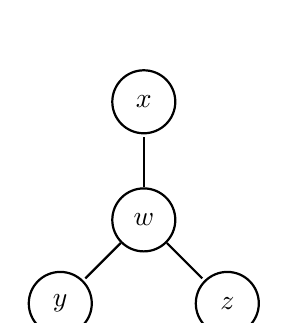
\begin{tikzpicture}[-,>=stealth',shorten >=1pt,minimum size=0.8cm,scale=.1,node distance=1.5cm, thick]
	\node[circle,draw] (A) 						{$w$};
	\node[circle,draw] (B) [above of=A] 		{$x$};
	\node[circle,draw] (C) [below right of=A] 	{$z$};
	\node[circle,draw] (D) [below left of=A] 	{$y$};
	
	\path 
	(A) edge	(B)
	(A) edge	(C)
	(A) edge	(D)
	;
\end{tikzpicture}
\caption{\label{fig:simple-MRF}Illustration of a simple MRF corresponding to distributions over 4 random variables admitting the following factorisation structure:\\ $p(w,x,y,z)\propto \psi_{w}(w)\psi_{x}(x)\psi_{y}(y)\psi_{z}(z)\psi_{wx}(w,x)\psi_{wz}(w,z)\psi_{wy}(w,y)$.}
\end{figure}
%The node potentials usually correspond to the likelihood of some observations $y_i$ (possibly a collection of observations) such that they can be written
%\eqa{ \psi_i(x_i) &=& p_i(y_i\st x_i),	\nn	}
%for some likelihood model $p_i$.
In this work, we are mainly concerned in determining or approximating  \emph{marginals}\margnote{marginals} on the MRF i.e. the distributions $p_{\mathcal I}(x_{\mathcal I})$ for $\mathcal I\subseteq\mathcal V$  with
\eqa{		p_{\mathcal I}(x_{\mathcal I}) &:=& \int p(x_{\mathcal V\backslash \mathcal I})\dx_{\mathcal V\backslash\mathcal I}	\label{eq:marginals}.}
A particular case of interest is $\mathcal I=\{r\}$ corresponding to the case of singleton marginals.\add{Discuss why} The integrals of the form \eqref{eq:marginals} are typically intractable but exploiting the underlying factorisation structure can lead to good approximation methods.

We distinguish between two classes of undirected graph structures: the connected acyclic ones (\emph{trees}) and the rest (\emph{loopy graphs}). As the rest of this document will make clear, in comparison to loopy graphs, computing marginals on a tree is relatively simple. Among the trees, two graph structures are of particular interest in this document: the \emph{chain graph} and the \emph{star graph}. We also illustrate one specific type of loopy graph: the \emph{grid graph}.

%\dred{COULD ADD hierarchical model as tree graph}

%%%%%%%%%%%
\subsection{Examples of MRF}
In this point, we present a brief overview of three examples of graph structures on which we will focus most of our effort throughout this document. We also present the type of applications they are connected with. They will be considered in more details in subsequent sections.\add{check, come back}

%%%%%%%%%%%%%%
\subsubsection{Hidden Markov Models}
Chain graphs form the underlying structure of \emph{Hidden Markov Models} (HMM)\margnote{HMM}. These can be illustrated as follows:
\begin{figure}[!h]
\center
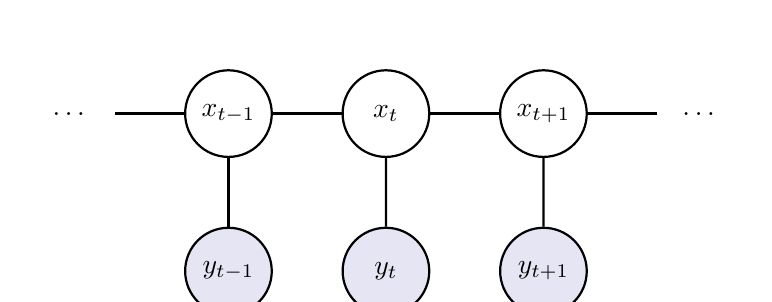
\begin{tikzpicture}[-,minimum size=1.1cm,scale=.1,node distance=2cm, thick]
	\node[circle,draw] (A) {$x_{t-1}$};
	\node[circle,draw] (B)[right of=A] {$x_{t}$};
	\node[circle,draw] (C) [right of=B] {$x_{t+1}$};
	\node[] (D) [right of=C] 	{$\dots$};
	\node[] (E) [left of=A]		{$\dots$};
	\node[circle,fill=DarkBlue!10,draw] (F) [below of=A] {$y_{t-1}$};
	\node[circle,fill=DarkBlue!10,draw] (G) [below of=B] {$y_{t}$};
	\node[circle,fill=DarkBlue!10,draw] (H) [below of=C] {$y_{t+1}$};
	
	\path 
	(A) edge	(B)
	(B) edge	(C)
	(C) edge	(D)
	(E) edge	(A)
	(A) edge (F)
	(B) edge (G)
	(C) edge (H)
	;
\end{tikzpicture}
\caption{\label{fig: hmm1} HMM with states $\{x_{t}\}_{t=1}^{T}$ and observations $\{y_{t}\}_{t=1}^{T}$.}
\end{figure}

HMMs are used in a broad range of applications from modelling time series data to speech processing\add{cite stuff here}. In HMMs, the node potentials correspond to the likelihood of the corresponding observation and the edge potentials correspond to the \emph{transition density}:
\eqa{	\psi_t (x_t) &=& p(y_t\st x_t), \quad\text{and}\quad \psi_{t-1,t}(x_{t-1},x_t) \spe p(x_t\st x_{t-1}).	\nn}
A prior $p_{0}(x_{1})$ is assumed to be given for the first node so that $\psi_1(x_1) = p_{0}(x_1)p(y_1\st x_1)$. In this case, obtaining or approximating the singleton marginals is known as a \emph{smoothing problem}\margnote{smoothing}. The marginals or \emph{smoothing densities} can be written $p(x_t\st y_{1:T})$ to make explicit the dependence on all available observations.

A particular case is the \emph{filtering problem}\margnote{filtering} where one is only interested in building the last singleton marginal or, to put the problem in the same framework as before, to build marginals taking only into account the observations available until the point considered. The densities of interest can therefore be written $p(x_t\st y_{1:t})$.
%This is particularly relevant for applications such as time series analysis.\\

The \emph{linear-Gaussian} case is a particular instance of HMM, usually expressed as:
\eqa{	\syst{
			p_{0}(x_1) 				&=& \mathcal N(x_1; \mu_0, Q_0)	 	\\
			p(x_t\st x_{t-1}) 	&=& \mathcal N(x_t; A_t x_{t-1}+a_t, Q_t)		\\
			p(y_t\st x_t) 		&=& \mathcal N(y_t; B_t x_t+b_t, R_t)
		}
	\nn}
where $\mu_0$ as well as the $Q_i$, $R_i$, $A_i$, $a_i$, $B_i$ and the $b_i$ are deterministic. In such a case, an analytical expression for both the filtering and the smoothing densities can be obtained through the well-known \emph{Kalman filter} and \emph{smoother} (see for example \citet{anderson79}). 

In the general case however (nonlinear and/or non-Gaussian), these densities are typically intractable. Approximation algorithms such as \emph{sequential Monte Carlo} (SMC)\margnote{SMC} methods can then be used. \add{link to section where discussed} 
%We will show in this document a novel method to exploit a variational method known as \emph{expectation propagation} to help the performances of SMC smoothing algorithms. \dred{ADD SECTION NUMBER}

%%%%%%%%%%%%%%
\subsubsection{Star graphs}

In this document, we define \emph{star graphs}\margnote{star graph} as corresponding to a structure with a single random variable (possibly high-dimensional) with a node potential that factors into several likelihood terms. The structure is illustrated in the \fig{fig:star1}. 

\begin{figure}[!h]
\center
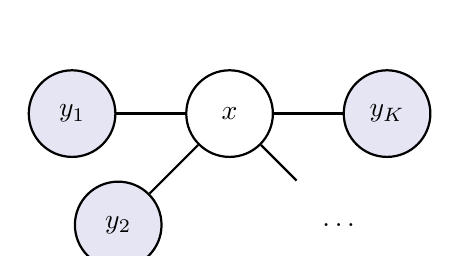
\begin{tikzpicture}[-,minimum size=1.1cm,scale=.1,node distance=2cm, thick]
	\node[circle,draw] (A) {$x$};
	\node[circle,fill=DarkBlue!10,draw] (B) [left of=A]		   {$y_{1}$};
	\node[circle,fill=DarkBlue!10,draw] (C) [below left of=A]  {$y_{2}$};
	\node[] (D) [below right of=A] {\dots};
	\node[circle,fill=DarkBlue!10,draw] (E) [right of=A]  {$y_{K}$};
	
	\path 
	(A) edge	(B)
	(A) edge	(C)
	(A) edge	(D)
	(A) edge (E)
	;
\end{tikzpicture}
\caption{\label{fig:star1} Star graph with hidden state $x$ and observations $\{y_k\}_{k=1}^{K}$. }
\end{figure} 

In this case, the singleton marginal can be written as:
\eqa{	p(x\st y) &\propto& \pi_0(x) \prod_{i=1}^{K} p(y_k\st x)	\nn}
where the $y_k$ are subsets of the entire observed data and $\pi_0$ is a prior on the hidden state. This can be a useful representation for distributed inference where each of the observation node can correspond to a distinct physical machine with a portion of the relevant data.\add{add link to section}\check{jun21}% We exploited this structure to come up with a novel way to perform distributed Bayesian inference. \dred{ADD SECTION NUMBER}

\subsubsection{Grid and loopy graphs}
The examples listed above do not exhibit cycles. An example of a common structure with cycles which is encountered, for instance, in image processing, is the \emph{grid graph}\margnote{grid graph} illustrated in \fig{fig:grid1} \citep{blake11}.

\begin{figure}[!h]
	\center
	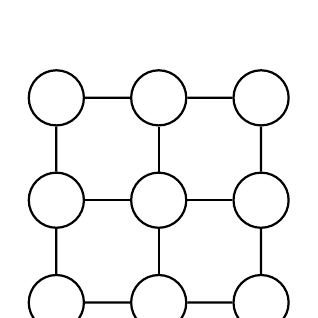
\begin{tikzpicture}[-,minimum size=.7cm,scale=.1,node distance=1.3cm, thick]
		\node[circle,draw] (A){};
		\node[circle,draw] (B) [left  of=A] {};
		\node[circle,draw] (C) [right of=A]{};
		\node[circle,draw] (D) [below of=A]{};
		\node[circle,draw] (E) [above of=A]{};
		\node[circle,draw] (F) [above of=B]{};
		\node[circle,draw] (G) [above of=C]{};
		\node[circle,draw] (H) [below of=B]{};
		\node[circle,draw] (I) [below of=C]{};
		\path
		(A) edge (B)
		(A) edge (C)
		(A) edge (D)
		(A) edge (E)
		(B) edge (F)
		(B) edge (H)
		(C) edge (I)
		(C) edge (G)
		(F) edge (E)
		(E) edge (G)
		(H) edge (D)
		(D) edge (I)
		;
	\end{tikzpicture}
\caption{\label{fig:grid1} Generic structure of a grid graph.}
\end{figure}

In image processing, grid graphs can be used to model interaction between the pixels of an image. In the case of image denoising for example, for each pixel $k$ a noisy value $y_k$ is observed and we can have a model for the likelihood of $y_k$ given the true pixel value $x_k$ in the form $p(y_k\st x_k)$. These then form the node potentials. 
Additionally, we may have a similarity measure which can be used to penalise neighbouring pixels being very dissimilar. These form the edge potentials.\\
The problem of finding or approximating the singleton marginals then corresponds to finding the likelihood of a particular pixel taking a specific value given all the noisy observations available.\check{jun21}\add{maybe link to relevant section} %\dred{ADD SECTION NUMBER WHERE WE SHOW HOW TO DO THIS}

\fi

%%%%%%%%%%%%%%%%%%%%%%%%%%
\part{Sampling Algorithms} % part I

%%%%%%%%%%%%%%%%%%%%
\chapter{Background}

\ifbgs% !TEX root = ../thesis.tex

In this chapter, we start with a brief overview of Monte Carlo estimators and associated sampling methods focusing in particular on Sequential Monte Carlo methods for the smoothing and filtering problem on Hidden Markov Models. We also introduce an alternative class of methods relying upon Piecewise Deterministic Markov Processes and in particular the Bouncy Particle Sampler (BPS). 

\section{\label{sec:MC+SMC}Monte Carlo Methods}
In this section we review briefly the foundations of Monte Carlo methods as well as a few key algorithms which will be discussed in the rest of the document.

\subsection{From quadrature to sampling}
% KEEP pi (later p is filtering/smoothing)
We consider the problem of computing the expected value of a test function $\varphi$ taking value over a space $\mathcal X$ with respect to a distribution $\pi\in\mathcal P(\mathcal X)$ i.e.: $I:=\E_\pi[\varphi(X)]$. Assuming it cannot be computed analytically, a general approach is to consider a quadrature rule of the form:
%
\eqa{
	I\esp\approx\esp \widehat I_N &=& \sum_{i=1}^{N} w(X^{(i)}) \varphi(X^{(i)})
}
%
for some fixed points $X^{(i)}\in\mathcal X$ and corresponding weights $w(X^{(i)})\in\mathbb R_+$. 
When the number of dimensions is low, we can consider deterministic quadrature rules such as the Gauss-Hermite quadrature (see e.g.: \citet{davis75}). However, as the dimensionality increases, the performance of these deterministic rules becomes catastrophic even for a large number of integration points (a well-known effect related to what Bellman called the \emph{curse of dimensionality} in dynamic programming \citep{bellman57,bengtsson08}). 
In such cases, a broadly studied approach is the Monte Carlo integration with
%
\eqa{	
	X^{(i)}\esp \simiid\esp \pi,\quad\text{and}\quad w(X^{(i)})\spe N\inv. 	
\label{eq:mcsampling}}
%
The strong law of large numbers then indicates that $\widehat I_N\to I$ almost surely with approximation error scaling like $\mathcal O(N^{-1/2})$ independently of the dimensionality of the problem (see e.g. \cite{robert04}). This is to be compared with deterministic rules which typically have approximation error scaling like $\mathcal O(N^{-\alpha/d})$ for a fixed $\alpha>0$ depending on the quadrature rule \citep{caflisch98}. The problem then becomes one of drawing iid samples from $\pi$ which is often also an intractable problem. Note that \eqref{eq:mcsampling} in fact defines an \emph{empirical measure} $\hat \pi$ with
%
\eqa{
	\hat \pi(x) &:=& N\inv\sum_{i=1}^{N} \delta_{X^{(i)}}(x),
}
%
and computing $\hat I_{N}$ amounts to taking the expected value of $\varphi(X)$ with respect to $\hat\pi$.\check{paragraph jul16}

%%%%%%%%%%%%%%%%%%%
\subsection{Importance sampling}
%For this point, we refer to the note by \citet{doucet11} and also to \citet[chapter 3.3 and 14.3]{robert04}.
In \emph{importance sampling} (IS), samples are drawn from a \emph{proposal distribution} $q\in\mathcal P(\mathcal X)$ that is easy to sample from (e.g.: a Gaussian) and is similar to the target distribution $\pi$. 
The quadrature weights are then adjusted to reflect that the samples are not drawn from the true distribution:
%
\eqa{
	X^{(i)}\esp \simiid\esp q(\cdot), \quad\text{and}\quad w(X^{(i)})\esp\propto\esp W(X^{(i)})\spe {\pi(X^{(i)})\over q(X^{(i)})},\label{eq:impsampling}
} 
%
where the weights $w(X^{(i)})$ are normalised to sum up to one.

Provided the support of $q$ includes that of $\pi$ i.e., $\pi(x)>0\Rightarrow q(x)>0$, the resulting \emph{importance sampling estimator} is consistent. Further, the estimator of the expected value of a specific test function $\varphi$ is finite provided $\E_{\pi}[\varphi(X)^{2}w(x)]<\infty$ \citep[chapter 3.3]{robert04}. Note that \eqref{eq:impsampling} also defines an empirical measure $\hat\pi$ with
%
\eqa{
	\hat\pi(x) &\propto& \sum_{i=1}^{N} W(X^{(i)})\delta_{X^{(i)}}(x).
}
%
 

%%%%%%%%%%%%%%%%%%%
\subsubsection{Effective sample size}
One way to assess the quality of an importance sampling estimator is to consider the ratio of the variance of the corresponding Monte Carlo estimator and the variance of the IS estimator. The general ratio is hard to handle and depends upon the test function with respect to which the expected value is computed. \citet{kong92} suggested considering the following proxy known as the \emph{effective sample size}:
%
\eqa{
	\text{ESS} &=& {N\over 1+\V_{q}[W(X)]},
}
%
where $\V_{q}[W(X)]$ is the variance of the importance sampling weights. Using the sample variance of the normalised weights and simplifying the expression, the proxy that is usually considered for the ESS nowadays is
%
\eqa{
	\text{ESS} &=& \pat{\sum_{i=1}^{N}w(X^{(i)})^{2}}^{-1}\label{eq:ESS}.
}
%
This metric is bounded from below by $1$ -- the degenerate case where a single particle is carrying all the weight -- and from above by $N$ -- the ideal case where the samples are comparable to ideal Monte Carlo samples. \check{par jul16}

\subsection{\label{point:classical-sampling}Classical sampling algorithms}

In this point we mention briefly a few standard algorithms used to attempt to generate samples from a distribution.
Later on, we will compare alternative methods to these standard algorithms.
The list and descriptions are not meant to be exhaustive and we refer to \citet{robert04, green15} for a more complete overview.

\subsubsection{Metropolis-Hasting}
The Metropolis-Hasting algorithm (MH) is one of the most prominent member of the class of Markov Chain Monte Carlo methods (MCMC). In MCMC methods, one considers a sequence (chain) of random variables $X^{(1)}, X^{(2)},\dots$ following a conditional probability density or \emph{transition kernel} $K$ with $X^{(n+1)} \sim K(X^{(n)}, \,\cdot\,)$. 
The kernel is chosen in such a way that the chain admits a stationary distribution, i.e.: a distribution $\pi$ such that for $n$ large enough, $X^{(n)}\sim \pi$ implies that $X^{(n+1)}\sim\pi$. Further, the kernel is chosen in such a way that the stationary distribution corresponds to the target distribution.

The MH algorithm corresponds to the transition kernel below where $q$ is a proposal distribution and $p_{u}$ is the (unnormalised) target \citep[chapter 6]{robert04}.

\begin{algorithm}[!h]\small
	\caption{\label{alg:mh-kernel}\dblue{\emph{\small Metropolis-Hasting transition}}}
	\begin{algorithmic}[1]
		\State generate $Y^{(n)}\sim q(\cdot | X^{(n)})$
		\State compute the acceptance rate
			$$ \rho \leftarrow \min\left\{ {p_{u}(Y^{(n)})\over p_{u}(X^{(n)})}{q(X^{(n)}|Y^{(n)})\over q(Y^{(n)}|X^{(n)})}, 1\right\} $$
		\State generate $\beta\sim \mathcal B(\rho)$ (Bernoulli)
		\State compute the new state: $X^{(n+1)} \leftarrow \beta Y^{(n)} + (1-\beta)X^{(n)} $
	\end{algorithmic}
\end{algorithm}

In the MH algorithm, different choices of $q$ will lead to different algorithms that may be easier or harder to implement. For example taking a \emph{symmetric} proposal with $q(x|y)=q(y|x)$ leads to a simplified acceptance ratio (see \citet{green15} for a discussion).

\subsubsection{Gibbs sampling}

Gibbs sampling can be applied when targeting a multivariate distribution $p\in \mathcal P(\mathcal X)$ where $\mathcal X$ is $d$-dimensional and where it is possible to generate samples from the target's full conditionals $p_{1}, \dots, p_{d}$ \citep[chapter 7]{robert04}.

\begin{algorithm}[!h]\small
	\caption{\label{alg:gibbs-alg}\dblue{\emph{\small Gibbs iteration}}}
	\begin{algorithmic}[1]
		\State given $x^{(n)}=(x_{1}^{(n)},\dots,x_{d}^{(n)})$
		\For{$k=1:d$}
			\State generate $X^{(n+1)}_{k} \sim p_{k}(x_{k}\st x^{(n)}_{-k})$ \,\,with $x_{-k}^{(n)}:=(x_{1}^{(n+1)},\dots,x_{k-1}^{(n+1)},x_{k+1}^{(n)},\dots,x_{d}^{(n)})$
		\EndFor
	\end{algorithmic}
\end{algorithm}

The potential advantage of the method is that, at any given point, it only considers uni-dimensional distributions. 
The major disadvantage of the method is that it goes sequentially over each dimensions rendering the method extremely slow as soon as the dimensionality of the target distribution becomes substantial.


\subsubsection{Hamiltonian Monte Carlo sampling}

The Hamiltonian Monte Carlo method (HMC) generates samples along a trajectory on the the parametric surface $(x, -U(x))$ where $-U(x):=\log \pi_{u}(x)$ and $\pi_{u}$ is the (unnormalised) target distribution.
The trajectory can be interpreted as the time evolution of a specific physical system described by a Hamiltonian depending on the target distribution (potential) and a momentum term encouraging exploration of the state-space (kinetic energy) with \emph{momentum variable} $p$. The Hamiltonian is defined as
\eqa{
	H(x, p) &:=& U(x) + \frac12\scal{p, M\inv p} 
}
where $M$ is a mass matrix that can be set to the identity or adjusted depending on knowledge of the problem's geometry \citep{betancourt17, barp18}. 
Since finding the exact trajectory of a Hamiltonian system is usually intractable, numerical integrators can be used and the leapfrog method is often used in HMC.

\begin{algorithm}[!h]\small
	\caption{\label{alg:hmc-alg}\dblue{\emph{\small HMC iteration}}}
	\begin{algorithmic}[1]
		\State draw a momentum variable $P^{(n)}\sim\mathcal N(0, M) $
		\State compute $L$ steps of the leapfrog integrator from $(X^{(n)},P^{(n)})\rightarrow (X^{\star},P^{\star})$ 
		\State compute the acceptance ratio
			$$ \rho \leftarrow \min\left\{\exp\left(-\Delta H \right),1\right\} $$
			where $\Delta H \leftarrow H(X^{\star},P^{\star})-H(X^{(n)}, P^{(n)})$.
		\State generate $\beta \sim\mathcal B(\rho)$
		\State compute the new state: $X^{(n+1)} \leftarrow \beta X^{\star}+(1-\beta)X^{(n)}$
	\end{algorithmic}
\end{algorithm}

This method generates a Markov chain with stationary distribution corresponding to the target distribution $\pi$. 
It is a very popular method in computational Bayesian inference and tends to be preferred over approaches such as the MH algorithm \citep{neal11}. We will show later in chapter \ref{chapBPSMRF} than in some cases a method that exploits the factorisation structure of the target distribution explicitly may lead to better results. 

\newpage
%%%%%%%%%%%%%%%%%%%%%%
\section{Sequential Monte Carlo Methods}
%%%%%%%%%%%%%%%%%%%%%%
\subsection{Sequential importance sampling}
%%%%%%%%%%%%%%%%%%%
%\subsubsection{Hidden Markov models}
In the context of HMMs, we are usually interested in estimating a sequence of target distributions $\{\pi_{t}(x_{1:t})\}_{t=1}^{T}$ which admit the following factorisation structure:
%
\eqa{
	\pi_{t}(x_{1:t}) &\propto& \pi_{t}(x_{t}\st x_{1:t-1})\pi_{t-1}(x_{1:t-1}).\nn
}
%
This led to the development of \emph{sequential Monte Carlo} (SMC) methods \citep[chapter 14.3]{robert04}. The underlying principle of sequential importance sampling is the same as that of importance sampling except that a different proposal is considered at every step $t$ taking into account the previous draw of particles and the evolution of the system:
%
\eqa{
	q_{t}(x_{1:t}) &\propto& q_{t}(x_{t}\st x_{1:t-1})q_{t-1}(x_{1:t-1}).	\nn
}
%
Following this form, new samples or \emph{particles} $X^{(i)}_t$ can be drawn from $q_{t}(x_{t}\st X^{(i)}_{1:t-1})$ and the weights corresponding to the trajectories $\{X^{(i)}_{1:t}\}$ then need to be multiplied by a factor $\alpha^{(i)}_{t}$ with\check{jul16, jun24}
%
\eqa{
	\alpha^{(i)}_{t} := {\pi_{t}(X^{(i)}_{1:t} )\over \pi_{t-1}(X^{(i)}_{1:t-1}) q_{t}(X^{(i)}_{t}\st X^{(i)}_{1:t-1})}.
}
%
The variance of an IS estimator is directly related to the variance of the associated importance weights. In order to counter the increase of variance induced by the sequential IS procedure, the proposal at step $t$ should be such that the variance of the update factors $\alpha_t$ is as small as possible. In particular, the \emph{optimal proposal} \citep{doucet11} keeps it at zero with
\eqa{		q^{\text{opt}}_{t}(x_{t}\st x_{1:t-1}) &:=& \pi_{t}(x_{t}\st x_{1:t-1}).	\label{optimal proposal}}
Additionally, since we cannot typically sample easily from the optimal proposal, we have to resort to approximating distributions.\check{jul16, jun24}

%%%%%%%%%%%%%%%%%%%%%%%%%%%%%%%
\subsection{Particle filtering}
In the filtering problem on a HMM, the target densities are $\pi_{t}(x_{1:t})=p(x_{1:t}\st y_{1:t})$ and their marginals. The incremental update factors are given by
\eqa{ \alpha_t(x_{1:t}) &=& {p(x_{1:t}\st y_{1:t})\over p(x_{1:t-1}\st y_{1:t-1})q_t(x_t\st x_{1:t-1})} 	\nn\\
	&=& {p(x_t,y_t\st x_{1:t-1},y_{1:t-1})p(x_{1:t-1}\st y_{1:t-1})p(y_{1:t-1})\over p(x_{1:t-1}\st y_{1:t-1})q_t(x_t\st x_{1:t-1})p(y_{1:t})}  \nn\\
	&\propto& {p(y_t\st x_t)p(x_t\st x_{t-1}) \over q_t(x_t\st x_{1:t-1})},}
where we exploited the conditional dependence structure of the HMM. 
Consequently, the optimal proposal is
\eqa{		q^{\text{opt}}_{t}(x_{t}\st x_{t-1}) &\propto& p(y_{t}\st x_{t})p(x_{t}\st x_{t-1})	, \label{particle filter OID}}
which could also have been obtained from applying \eqref{optimal proposal}.\\
Beyond simply corresponding to sequential importance sampling for the filtering problem, the particle filter adds an extra step: resampling. 
This step alleviates the problem of weight degeneracy whereby the variance of estimators grows over time when one considers a suboptimal proposal distribution such as the bootstrap proposal. 
The resampling step consists of resampling particles with replacement depending upon their weights.
This, in practice, is done when the ESS comes under a pre-assigned threshold \citep{delmoral06}.
Several schemes exist with the simplest one being the \emph{Multinomial Resampling} where $n$ particle indices are drawn from a Multinomial with weights corresponding to the $n$ weights of the initial particles.\\
Resampling is a crucial step needed to make SMC methods viable \citep{hol06, doucet11}. However, the methods discussed in this thesis do not depend upon the resampling scheme and therefore we will assume in the sequel that a resampling scheme is applied without discussing it further. In the experiments we use the standard multinomial resampling.

%We have omitted the \emph{resampling step} in algorithm \ref{alg:particle-filter}. That step resamples particles with replacement based on their weights if the ESS comes under a pre-assigned threshold \citep{delmoral06}. In practice, this alleviates the problem of weight degeneracy incurring growth of variance over time when one considers a suboptimal proposal distribution such as the bootstrap proposal. Although this step is a key aspect of particle filters, it is not an aspect that plays an important role in the issues we consider in this document; in the sequel we will therefore assume that a standard multinomial resampling is applied \citep{hol06,doucet11}. 

A skeleton of a particle filter algorithm is given below.\check{jun24}
%
\begin{algorithm}[!h]\small
	\caption{\label{alg:particle-filter}\dblue{\emph{\small Particle filter}}}
	\begin{algorithmic}[1]
		\State sample $X_{1}^{(i)}\simiid q_{1}$ for $i=1,\dots,N$	%\Comment{\emph{Initialization}}
		\State compute and normalise the weights $w_{1}(X^{(i)}_{1})\propto {\pi_{0}( X^{(i)}_{1})p(y_{1}\st X^{(i)}_{1})/ q_{1}(X^{(i)}_{1})}$
%		\State resample: $\{\X^{(i)}_{1},W^{(i)}_{1}\}\rightarrow\{\overline \X^{(i)}_{1},N\inv\}$\Comment{\emph{Using some resampling scheme}}\vspace*{.2cm}
		\For{$t=2:T$}
			\State sample $X^{(i)}_{t}\simiid q_{t}( \cdot \st X^{(i)}_{t-1}, y_{t})$ with $q_{t}\approx q_{t}^{\text{opt}}$ for $i=1,\dots,N$
			\State update and normalise the weights $w^{(i)}_{t}\propto\alpha^{(i)}_{t}w^{(i)}_{t-1}$
			\State resample the particles if necessary
		\EndFor\\
		\Return weighted set of particles $\{X^{(i)}_{1:T},w^{(i)}_{1:T}\}_{i=1}^{N}$
	\end{algorithmic}
\end{algorithm}
%

The computational complexity of algorithm \ref{alg:particle-filter} is $\mathcal O(TN)$. Indeed, at each step $t$,  the algorithm samples $N$ particles and computes their corresponding weights which has linear complexity in the number of particles.\check{jun24}

Sampling directly from the optimal proposal is often an intractable problem by itself. In the context of filtering, an alternative choice is the \emph{bootstrap proposal} \citep{doucet11} with
\eqa{q^{\text{bs}}(x_{t}\st x_{t-1})&:=&p(x_{t}\st x_{t-1}),}
which is often easier to sample from. In that case, the update factor simply reduces to $\alpha^{(i)}_t \propto p(y_t\st X^{(i)}_t)$. However, since the likelihood and the transition density may not be well aligned, those update factors can vary a lot incurring an increase in the variance of the resulting estimator.
This problem is particularly prevalent in high dimensions when the distributions considered tend to be more concentrated.

%\check{jul16}

\subsection{\label{bg:particle-smoothing}Particle smoothing}

In the smoothing problem on a HMM, the target densities are $p(x_t\st y_{1:T})$. These densities can be expressed as the marginals of joint densities over subsequent states: 
\eqa{p(x_t\st y_{1:T})&=&\int p(x_t,x_{t+1}\st y_{1:T})\,\mathrm{d}x_{t+1}.\nn} Exploiting the conditional dependence structure of the HMM, the integrand can be factorised leading to
\eqa{	p(x_t\st y_{1:T}) &=& \int p(x_t\st x_{t+1},y_{1:t})p(x_{t+1}\st y_{1:T})\,\mathrm{d}x_{t+1}	\nn\\&=& p(x_t\st y_{1:t}) \int {p(x_{t+1}\st x_t)\over p(x_{t+1}\st y_{1:t})}p(x_{t+1}\st y_{1:T}) \,\mathrm{d}x_{t+1}.\label{eq FFBS}}
This relation leads to the \emph{forward filtering, backward smoothing} (FFBS) algorithm \citep{hurzeler98, doucet00}.
Plugging the particle approximation to the filtering distribution in equation \eqref{eq FFBS} gives:
\eqa{		
	\hat{p}(x_{t}\st y_{1:T}) &=& \hat{p}(x_{t}\st y_{1:t})\int {p(x_{t+1}\st x_{t})\over \int p(x_{t+1}\st x_{t})\hat p(x_{t}\st y_{1:t})  \dx_{t}}\hat p(x_{t+1}\st y_{1:t+1})\dx_{t+1}\nn \\
			&= &	\sum_{i=1}^{N}w^{(i)}_{t\st T}\delta_{X^{(i)}_{t}}(x_{t}),	}
where the smoothing weights are given recursively by
\eqa{		w^{(i)}_{t\st T} &\propto& w^{(i)}_{t}\sum_{j=1}^{N}{w^{(j)}_{t+1\st T}\pac{p(X^{(j)}_{t+1}\st X^{(i)}_{t})\over \sum_{k=1}^{N}w^{(k)}_{t}p(X^{(j)}_{t+1}\st X^{(k)}_{t})}}. \label{eq FFBS weights}	}
In essence, the FFBS algorithm simply recycles a particle filter updating its weights according to equation \eqref{eq FFBS weights}. \check{jul16}

The computation of the updated smoothing weights has complexity $\mathcal O(TN^{2})$ since, at each step, we need to consider the matrix of all pairwise interactions between the particles at two subsequent steps: $[p(X^{(j)}_{t+1}\st X^{(i)}_{t})]_{i,j=1}^{N}$. Since the FFBS algorithm recycles the particles from a particle filter, the performances of the resulting estimators can suffer if the support of the filtering distribution at step $t$ is significantly distinct from that of the smoothing distribution at step $t$.\check{jul16, jun29,jun24}




%%%%%%%%%%%%%%%%%%%%%%%%%%%%%%%%%%%%%%%%%%%%%%%%%%%%%%%%%%%%%%%%
\section{\label{point:BPS}Sampling with Piecewise Deterministic Markov Processes}
The \emph{Bouncy Particle Sampler} (BPS) of \citet{bouchard15} is inspired from an algorithm in the physics literature \citep{peters12} and belongs to a wider class of sampling methods based on Piecewise Deterministic Markov Processes (PDMP) \citep{bierkens16, bierkens17, wu17, vanetti17}.

The BPS algorithm considers a target distribution $\pi$ on $\R^{d}$, proportional to a non-negative function $\gamma$ which can be evaluated pointwise: $\pi(x) = Z\inv \gamma(x)$
but the normalisation constant $Z$ is intractable. 
The objective is again the computation of expected values of the form $\E_\pi[\varphi]$ for an arbitrary test function $\varphi:\R^{d}\to \R$. 

Defining the \emph{energy} function $U$ as $U(x) = -\log \gamma(x)	$
 and assuming it is continuously differentiable, the algorithm generates a piecewise linear path based on $\nabla U$. 
 Each segment is specified by an initial position $x^{(i)}\in \R^{d}$, a length $\tau_{i+1}\in \R^{+}$ and a velocity $v^{(i)}$ with the recurrence $x^{(i+1)}=x^{(i)}+v^{(i)}\tau_{i+1}$. The times where the velocity changes are given by the cumulative sums, $t_i=\sum_{j=1}^{i}\tau_j$ with $t_0=0$. The continuous positions along the path are therefore given by
\eqa{	x(t) &=& x^{(i)} + v^{(i)}(t-t_i), \quad\text{for}\quad t\in[t_i,t_{i+1}).	\label{eq:path-BPS}}
The authors show that, if the lengths $\{\tau_{i}\}_{i\ge 1}$ are governed by a specific Inhomogenous Poisson Process (IPP) and if the speeds are modified for each segment according to a simple reflection mechanism, then the target expected values can be approximated consistently via an integral of the test function along the path given by \eqref{eq:path-BPS}.

In the BPS algorithm, the IPP governing the lengths of the trajectory segments has intensity function $\lambda:\R^{d}\times\R^{d}\to\R^{+}$ with
%
\eqa{
	\lambda(x,v) &=& \scal{\nabla U(x),v}^{+}.	
}
%
At the end of each segment, the trajectory ``bounces'' and the velocity is reflected against the local level set of the energy $U$:
\eqa{	v' &=& R(x)v \spe v-2{\scal{\nabla U(x),v}\nabla U(x)\over \bnorm{\nabla U(x)}^{2}}.	}
The authors show that the velocities also need to be ``refreshed'' according to the arrival times of a (homogenous) Poisson process (PP) of intensity $\lambda^{\text{ref}}\ge 0$, a parameter of the BPS. This ensures the algorithm explores the entirety of the space. The basic BPS algorithm is reproduced in \hyperref[alg:BPS1]{algorithm~\ref*{alg:BPS1}} below.

\clearpage

\begin{algorithm}[!h]\small
	\caption{\label{alg:BPS1}\small \idblue{Basic BPS}}
	\begin{algorithmic}[1]
	\State initialise $(x^{(0)},v^{(0)})$, set $T$, trajectory length, set $t=0$ and $i=1$
	\While{$t < T$}
		\State simulate first arrival time $\tau_{\text{bounce}} \sim \text{PP}(\chi(t))$  with
		$$ \chi(t) = \lambda(x^{(i-1)}+v^{(i-1)}t,v^{(i-1)})$$
		\State simulate $\tau_{\text{ref}}\sim \mathrm{Exp}(\lambda^{\text{ref}})$
		\State let $\tau_{i}\leftarrow \min(\tau_{\text{bounce}},\tau_{\text{ref}})$
		\State compute the next position $x^{(i)}\leftarrow x^{(i-1)}+v^{(i-1)}\tau_{i}$
		\If{$\tau_{i}=\tau_{\text{ref}}$}
			\State sample next velocity $v^{(i)}\sim \mathcal N(0,I)$		\ElsIf{$\tau_{i}=\tau_{\text{bounce}}$}
			\State reflect the velocity $v^{(i)}\leftarrow R(x^{(i)})v^{(i-1)}$
		\EndIf
		\State let $t\leftarrow t_{i}\leftarrow t_{i-1}+\tau_{i}$
		\State update $i\leftarrow i+1$
	\EndWhile
	\end{algorithmic}
\end{algorithm}

The target expectation can then be obtained by integrating the test function along the path thus generated:
\eqa{	\E_\pi[\varphi] &=& T\inv \int_0^{T} \varphi(x(t))\mathrm{d}t	\nn\\
&\approx& T\inv \pat{\sum_{i=1}^{n-1} \int_0^{\tau_i} \varphi(x^{(i-1)}+v^{(i-1)}s)\,\mathrm{d}s + \int_0^{t_n-T}\varphi(x^{(n-1)}+v^{(n-1)}s)\mathrm{d}s}. \nn}
The integrals in the sum can themselves be approximated if needed using quadrature.

As we saw, the algorithm requires to sample the first arrival time of an IPP of intensity $\chi(t)=\lambda(x+vt,v)$ where $\lambda(x,v)=\scal{\nabla U(x),v}^{+}$. Sampling from an IPP is a well explored topic in the literature and the authors summarise three possible approaches which we list briefly below:
%\begin{itemize}\itsep0

    \emph{Time-scale transformation}: this approach requires computing the inverse quantile of $\Xi(t):=\int_{0}^{t} \chi(s)\mathrm{d}s$ which is usually intractable but it can be computed numerically if the target is strictly log-concave and differentiable. Given $V$ drawn from a Uniform on $[0,1]$, the first arrival time of the IPP is given by $\Xi^{\inv}(-\log(V))$.
%This, the authors show, allows to make a connection with the Metropolis Hastings algorithm.
    
    \emph{Adaptive thinning}: this approach requires an upper bounds $\overline{\chi}_{s}(t)$ with $\overline\chi_{s}(t)=0$ for $t<s$ and $\overline\chi_{s}(t)\ge\chi(t)$ for $s\le t\le s+\Delta(s)$ where $\Delta$ is a positive function (in the standard case, $\Delta=+\infty$). Additionally, it requires the ability to sample from the IPP corresponding to $\overline\chi_{s}$. Let $\tau$ be such a sample with $\tau\le s+\Delta$, there is then an accept-reject step with rate $\chi(\tau)/\overline\chi(\tau)$. Ideally, $\Delta$ and $\chi/\overline\chi_{s}$ are large (so that we do not have to simulate too many candidates which would incur an increased computational cost).
 
    \emph{Superposition}: if the energy $U$ can be decomposed in a sum $U(x)=\sum_{j=1}^{m}U^{[j]}(x)$ and that each term can be targeted (via one of the first two methods), then we can use the thinning method with bound $\sum_{j=1}^{m}\chi^{[j]}(t)$.


%\section{Discussion}
%
%\todofr{
%\textbf{move this discussion where it belongs: at end of content chapters}
%	Connect the two background sections with main element (PF, PS link to HMM, PDMP, Local PDMP for anything. Exact methods.).
%}


\fi

%%%%%%%%%%%%%%%%%%%%%%%%%%%%%%
\chapter{Two Filter Smoothing}

\iftfs% !TEX root = ../thesis.tex

In this chapter, we focus on the problem of approximating the smoothing distributions for a Hidden Markov Model (HMM) with continuous state-space.
We assume that a sequence of empirical densities approximating the filtering distributions has already been obtained through a particle filtering step.
We had seen at point \ref{bg:particle-smoothing} that the \emph{forward filtering backward smoothing} (FFBS) algorithm can produce an approximation to the smoothing distributions by recycling a particle filter and updating its weights.  As shown in point \ref{bg:particle-smoothing}, the FFBS algorithm has quadratic complexity and may suffer from the lack of resampling step if the smoothing distribution and the filtering distribution have significantly different support. 

In this chapter, we introduce a class of algorithms that can be obtained from another factorisation of the smoothing distributions than that used to obtain the FFBS. We also introduce algorithms with a computational complexity that is sub-quadratic in $N$ and compare these algorithms in numerical experiments.

%%%%%%%%%%%%%%%%%%%%%%%%%%%%
\section{Two Filter Smoothing}


\subsection{\label{point:TFS}Two filter formula}
An alternative to the FFBS approach is to exploit the \emph{two filter formula}. 
To derive it, note that the smoothing distribution can be written in the following way using Bayes' formula:
%
\eqa{
	p(x_t\st y_{1:T})&=& {p(x_t,y_{1:t-1},y_{t:T})\over p(y_{1:T})}.\nn
	}
% 
Then, exploiting the conditional dependences of the HMM, we get
%
\eqa{
	p(x_t\st y_{1:T}) 	
		&\propto& p(y_{t+1:T}\st x_t,x_{t+1},y_t)p(y_t\st x_t,x_{t+1})
\nn\\
		&\propto& p(x_t\st y_{1:t-1})p(y_{t:T}\st x_t).	\label{eq:TFS}
}
%
This last factorised form is the two filter formula which leads to the \emph{two filter smoothing} (TFS) algorithm \citep{bresler86, kitagawa96}. 
The first term in \eqref{eq:TFS} is the prediction density (PD), 
the second term $p(y_{t:T}\st x_{t})$ is called the \emph{backward information filter} (BIF). To simplify developments we introduce the following non-standard notations for the predictive density and the backward information filter:\check{jul16}
%
\eqa{
	\pd_{t}(x_{t}) \esp:=\esp p(x_{t}\st y_{1:t-1}), \quad\text{and}  \quad \bif_{t}(x_{t}) \esp:=\esp p(y_{t:T}\st x_{t}).
}
%
The prediction density is obtained by integrating the filtering density multiplied by the transition density:
%
\eqa{
	\pd_{t}(x_{t}) &=& \int p(x_{t}\st x_{t-1})p(x_{t-1}\st y_{1:t-1})\dx_{t-1}.\label{eq:pred-dens}
}
%
an approximation to the prediction density can therefore easily be obtained by plugging a particle representation of the filtering density in \eqref{eq:pred-dens}. \check{jul16, july5}
%%%%%%%%%%%%%%%%%%%%%%%%%%
\subsection{Targeting the backward information filter}
The backward information filter cannot be directly targeted in a SMC framework in general as it may not be proportional to a distribution in $x_{t}$. 
In \citet{briers10}, the authors therefore suggest to introduce a sequence of artificial \emph{normalisation densities} $\{\gamma_{t}\}_{t=1}^{T}\in\mathcal P(\mathcal X)$ such that, for each step $t$, the product of $\gamma_{t}$ and $\bif_{t}$ is normalisable. 
In other words, the normalising distribution $\gamma_{t}$ allows to define a \emph{normalised backward information filter} in $\mathcal P(\mathcal X)$ with
%
\eqa{
	\tbif_{t}(x_{t}) &:=& Z\inv_{t}\gamma_{t}(x_{t})\bif_{t}(x_{t})
}
%
for some normalising constant $Z\inv_{t}$.\check{july5}
Any $\gamma_{t}\in\mathcal P(\mathcal X)$ can be chosen as long as it verifies the \emph{support condition} i.e.: as long as its support covers that of the backward information filter:
%
\eqa{	
	\bif_t(x_t) &>&0 \quad\Longrightarrow\quad \gamma_{t}(x_{t})\esp>\esp 0. \label{eq: tech condition normalisation density}	
}
%
In order to target the sequence of normalised BIF in a SMC framework, it is useful to show that it verifies a factorisation structure similar to that of the filtering distribution. For this, we start by noting that
%
\eqa{		
	p(y_{t:T}\st x_{t},x_{t+1}) 
		&=& p(y_{t+1:T}\st x_{t},x_{t+1},y_{t})p(y_{t}\st x_{t},x_{t+1})\nn\\
		&=& p(y_{t}\st x_{t}) \bif_{t+1}(x_{t+1}). \label{back rec 1}	
}
%
On the other hand, we also have that
%
\eqa{		
	p(y_{t:T}\st x_{t},x_{t+1}) 	
		&=& {p(y_{t:T},x_{t},x_{t+1})\over p(x_{t+1}\st x_{t})p(x_{t})}\nn\\
		&=&{p(x_{t+1}\st x_{t},y_{t+1:T})\text{BIF}_{t}(x_{t})\over p(x_{t+1}\st x_{t})},	\label{back rec 2}
}
%
where we have used the conditional independence structure of the HMM. 
Combining \eqref{back rec 1} and \eqref{back rec 2} then leads to\check{july5}
%
\eqa{	
	\bif_{t}(x_{t}) p(x_{t+1}\st x_{t},y_{t+1:T}) &=& p(y_{t}\st x_{t})p(x_{t+1}\st x_{t})\bif_{t+1}(x_{t+1}). 	\label{eq:tfs-bif2}
}
%
If we now introduce the normalisation densities $\gamma_{t}$ and $\gamma_{t+1}$ and the corresponding normalisation constants $Z_{t}$ and $Z_{t+1}$ in \eqref{eq:tfs-bif2} we get\check{july5}
%
\eqa{	 
	\tbif_{t}(x_{t})p(x_{t+1}\st x_{t},y_{t+1:T}) &=& 
		{Z_{t+1}\gamma_{t}(x_{t})\over Z_{t}\gamma_{t+1}(x_{t+1})}p(y_{t}\st x_{t})p(x_{t+1}\st x_{t})\tbif_{t+1}(x_{t+1}).		\nn
}
%
By construction of the normalisation densities, we can integrate the previous expression over $x_{t+1}$ to obtain
%
\eqa{		
	\tbif_{t}(x_{t}) &\propto& {\gamma_{t}(x_{t})}p(y_{t}\st x_{t})\int p(x_{t+1}\st x_{t}){\tbif_{t+1}(x_{t+1})\over \gamma_{t+1}(x_{t+1})}\dx_{t+1}.	\nn
}
%
Noting that $\bif_{T}(x_{T})=p(y_{T}\st x_{T})$ and iterating brings
%
\eqa{		
	\tbif_{t}(x_{t}) &=& \int {\gamma_{t}(x_{t})}\prod_{\ell=t}^{T-1}p(x_{\ell+1}\st x_{\ell})\prod_{k=t}^{T}p(y_{k}\st x_{k})\dx_{t+1:T}.	\nn
}
%
We can thus define a joint distribution $\tbif_{t}(x_{t:T})$ as the integrand of the above expression with the following sequential structure:
\eqa{		\tbif_{t}(x_{t:T}) &\propto& {\gamma_{t}(x_{t})p(x_{t+1}\st x_{t})p(y_{t}\st x_{t})\over \gamma_{t+1}(x_{t+1})}\tbif_{t+1}(x_{t+1:T}),	\label{recursion joint BIF}}
which lends itself well to the SMC framework with the optimal proposal:\check{jul16,july5}
%
\eqa{
	q^{\text{opt}}_{t}(x_{t}\st x_{t+1}) &\propto& {\gamma_{t}(x_{t})p(x_{t+1}\st x_{t})p(y_{t}\st x_{t})\over \gamma_{t+1}(x_{t+1})}.
}
%
%%%%%%%%%%%%%%%%%%%%%%%%%%%%%
\subsection{\label{introTFS}Two filter smoothing algorithm}
Plugging a particle representation of the filtering distribution in \eqref{eq:pred-dens}, the prediction density can be approximated by
%
\eqa{
	\widehat\pd_t(x_t)  &=& \sum_{i=1}^{N} w^{(i)}_{t-1}p(x_{t}\st X^{(i)}_{t-1}).	
\label{eq PDhat}	
}
%
Correspondingly, we can consider a particle representation of the normalised BIF obtained by following a backward particle filter with $M$ particles on \eqref{recursion joint BIF}. 
%The non-standard notation $\pd_{t}$ as well as the notations introduced below for the backward information filter will make the discussion of the TFS algorithm simpler and less cluttered. The backward information filter $\bif_t(x_t):=p(y_{t:T}\st x_{t})$ is not necessarily proportional to a distribution in $x_{t}$ and can thus not be directly targeted in a SMC context. However, one can define an auxiliary quantity by pre-multiplying the backward information filter by an artificial \emph{normalisation density} $\gamma_{t}(x_{t})$ such that the product
%%
%\eqa{		
%	\tbif_t(x_t) &:=& Z_{t}\inv{\gamma_{t}(x_{t}) p(y_{t:T}\st x_t)},		\label{def normalised BIF}
%}
%%
%is a distribution in $x_{t}$ (with $Z_{t}$ a normalisation constant) and can thus be targeted in the SMC framework \citep{briers10}.\check{jun24} 
%We will refer to these densities as \emph{normalisation densities}. The $\tbif_{t}$ are distributions and can be targeted in a SMC framework. 
Let us denote these by $\widehat\tbif_{t}$ with weights $\tilde w_{t+1}^{(j)}$ and particles $\tilde X^{(j)}_{t+1}$, i.e.:
%
\eqa{		
	\widehat\tbif_t(x_t) &=& \sum_{j=1}^{M} \tilde w^{(j)}_{t+1} \delta_{\tilde X^{(j)}_{t+1}}(x_{t}).
	} 
%
By dividing these by the corresponding normalisation density $\gamma_{t}$, we can obtain approximations to the original BIF:
%
\eqa{		
	\widehat\bif_t(x_t) &=& { \widehat\tbif_t(x_t)/  \gamma_{t}(x_{t})}.	\nn
}
%
Combining both the estimators of the prediction density and the backward information filter at step $t$, we can obtain a particle representation of the smoothing distribution with\check{jul5}
%
\eqa{		
	\hat{p}(x_{t}\st y_{1:T}) &=& \zeta_{t}\inv\widehat\pd_t(x_t)\widehat\bif_t(x_t)	, \label{first smoothing estimator}	
	}
%
where $\zeta_{t}$ is a normalisation constant.
That is a mixture of $NM$ terms and a further step may be desirable to reduce the number of components in the resulting representation of the smoothing distribution.
In particular, if we take $M=N$, at each step we have to consider a mixture with a quadratic number of terms in $N$ and this, independently of the choice of normalising densities meaning that the algorithm has inherently a quadratic complexity. We consider this choice in what follows.\check{jul16,jul5}
%Note that since both the predictive density and the normalised BIF have been approximated using $N$ particles, the above estimator is a mixture of $N^{2}$ components and a further resampling step can be applied to reduce it to a mixture of only $N$ components. %\add{This is what Fearnhead does}

%Another comment that we can make at this point is that the form of the estimator in \eqref{first smoothing estimator} suggests taking as normalisation densities the estimator of the prediction densities. \\

%We will show explicitly how to implement the two filter smoothing algorithm with a near-ideal normalisation density in \hyperref[sec:TFS]{section \ref*{sec:TFS}}. 


%\todofr{
%\begin{itemize}
%	\item Add here the algorithm
%	\item add short discussion (complexity, choice of normalisation)
%\end{itemize}
%}


%%%%%%%%%%%%%%%%%%%%%
\section{Backward Information Smoothing}
In this section, we explore the choice of normalisation densities and suggest using an approximation to the predictive density. It came to our knowledge that this choice had in fact also been studied independently and earlier than this work by \citet{taghavi12}. 
We show how the complexity of the resulting algorithm is quadratic in the number of particles. 
We also discuss two modified versions with sub-quadratic complexity. 
The first one, inspired by \citet{fearnhead10} and also discussed by \citet{taghavi12}, has linear complexity but the resulting estimators are not consistent. 
The second one, inspired by our paper \citep{lienart15}, has complexity $\mathcal O(NM)$ where $M$ is sub-linear in $N$ and leads to consistent estimators. \check{jul16}

%%%%%%%%%%%%%%%%%%%%%%%
\subsection{Choice of normalisation densities}
The choice of normalisation densities in the TFS algorithm is, in theory, only constrained by the support condition \eqref{eq: tech condition normalisation density}. However, the quality of the corresponding estimators for a finite sample size depends significantly on it. 
Combining \eqref{eq:TFS} and \eqref{recursion joint BIF}, we get
%
\eqa{
	p(x_{t}\st y_{t:T}) &\propto& {\pd_{t}(x_{t})\over \gamma_{t}(x_{t})} \int \tbif_{t}(x_{t:T}) \dx_{t+1:T}\nn
}
%
so that we can write
%
\eqa{		
	p(x_{t:T}\st y_{1:T}) &\propto& {\pd_{t}(x_{t})\tbif_{t}(x_{t:T})\over \gamma_{t}(x_{t})}	\label{normalised BIF and partial joint}.
}
%
This expression suggests picking $\gamma_{1}$ to be the prior distribution on the first state $\pi_{0}(x_{1})$ since that leads directly to 
%
\eqa{		
	p(x_{1:T}\st y_{1:T}) &=& \tbif_{1}(x_{1:T}).	\label{full joint and first bif}
	}
%
The last two equations \eqref{normalised BIF and partial joint} and \eqref{full joint and first bif} are crucial for the rest of the analysis. The first one suggests that if we pick $\gamma_{t}$ to be close to the predictive density then, then each term $\tbif_{t}(x_{t:T})$ forms an estimator for the partial joint smoothing densities $p(x_{t:T}\st y_{1:T})$; the second one indicates that upon selecting $\gamma_{1}$ to be the prior for the initial state, we end up targeting exactly the joint distribution of interest, no matter which admissible sequence $\{\gamma_{t}\}_{t=2}^{T}$ we picked earlier. \check{jul16}

This suggests to build a good estimator of the prediction density, based partly or entirely on a particle estimator of the filtering density; use it as normalisation density and target the corresponding normalised BIF recursively. 
We explored this idea and showed that it significantly outperforms the default choice used in \citep{briers10, fearnhead10} where the authors suggest also taking $\gamma_{1}$ as the prior $\pi_{0}$ and the subsequent $\gamma_{t}$ by propagating this through the dynamic of the HMM i.e.:
%
\eqa{
	\gamma_{t}(x_{t}) &=& \int p(x_{t}\st x_{t-1})\gamma_{t-1}(x_{t-1}) \mathrm dx_{t-1}\label{eq:choice-norma-bad}
}
%
Note that this choice also suffers from a tractability issue in a system with dynamic that is more complex than the linear and Gaussian one considered in \citep{fearnhead10} where, in any case, the optimal Kalman smoother should be preferred. We show in the appendix (point \ref{app:normalising-density-fearnhead-lg}) how this normalising density can be obtained in the case of a simple linear Gaussian dynamic.\check{jul16}

Upon selecting $\gamma_{t}$ to be the approximation of the predictive density \eqref{eq PDhat} based entirely on a a particle estimator of the filtering density, we get what Taghavi calls the \emph{backward informations smoothing} (BIS) algorithm \citet{taghavi12}. This choice verifies the support condition \eqref{eq: tech condition normalisation density} provided the support  of $p(x\st z)$ covers the support of the BIF. Typically, the support of $p(x\st z)$ is the whole space $\mathcal X$ which guarantees this.

The optimal importance function for targeting the corresponding normalised BIF is obtained by considering \eqref{recursion joint BIF} with this specific choice of normalising density:\check{jul16, jul2}
\eqa{		\tilde q^{\text{opt}}_{t}(x_{t}\st \tilde X^{(j)}_{t+1}) &\propto & {\hpd_{t}(x_{t})\over \hpd_{t+1}(\tilde X^{(j)}_{t+1})} p(\tilde X^{(j)}_{t+1}\st x_{t})p(y_{t}\st x_{t}),\label{eq:opt-prop-bif}}
where the $\{\tilde X_{t+1}^{(j)}\}_{j=1}^{N}$ are the particles from the previous smoothing step. These steps are illustrated in algorithm \ref{alg:bisquad}.\check{jul5}

%
\begin{algorithm}[!h]\small
	\caption{\label{alg:bisquad}\dblue{\emph{\small Backward information smoother with quadratic complexity}}}
	\begin{algorithmic}[1]
		\State run a PF targeting $\{p(x_{t}\st y_{1:t})\}_{t=1}^{T}$ with $N$ particles $\{X^{(i)}_{t}, w^{(i)}_{t}\}_{t,i=1}^{T,N}$
		\For{$t=T-1:2$}
			\State sample $\tilde X^{(j)}_{t}\simiid \tilde q_{t}(\cdot\st \tilde X^{(j)}_{t+1})$ with $\tilde q_{t}\approx \tilde q_{t}^{\text{opt}}$ for $j=1,\dots,N$
			\State update and normalise the weights $\tilde w^{(j)}_{t}\propto \tilde\alpha^{(j)}_{t}\tilde w^{(j)}_{t+1}$
		\EndFor
		\State same operations for $t=1$ but with $\tilde q^{\text{opt},i,j}_{1} \propto \pi_{0}(x_{1})p(\tilde X^{(j)}_{2}\st x_{1})p(y_{1}\st x_{1})/\hpd_{2}(\tilde X^{(j)}_{2})$\\

		\Return weighted set of particles $\{\tilde X^{(j)}_{1:T}, \tilde w^{(j)}_{1:T}\}$
	\end{algorithmic}
\end{algorithm}
%

At each step $t$ and for each particle $j$, the algorithm \ref{alg:bisquad} ideally requires sampling a particle from $\hpd_{t}(x_{t})p(\tilde X^{(j)}_{t+1}\st x_{t})p(y_{t}\st x_{t})$ which is a mixture of $N$ terms. Additionally, computing the updating factors for the weights requires computing a sum of $N$ terms $\hpd_{t+1}(\tilde X_{t+1}^{(j)})$. Provided we use $N$ particles to target the BIF, the complexity of the BIS algorithm is therefore inherently quadratic in the number of particles. This is the same computational complexity as that of the FFBS algorithm.\check{jul16, jul5}

As it is not trivial in general to sample from $p(\tilde X^{(j)}_{t+1}\st x_{t})p(y_{t}\st x_{t})$, let alone when it is combined with $\hpd_{t}(x_{t})$, a possibility akin to the bootstrap proposal for the particle filter is to simply sample from $\hpd_{t}(x_{t})$. The disadvantage is that this choice doesn't take into account all the information available (contained in $\tilde X^{(j)}_{t}$ and $y_{t}$). Assuming we can sample easily from the transition distribution, sampling from $\hpd_{t}$ can be done easily in two steps: first sample an index $i^{\star}\sim \mathcal M(w^{(1)}_{t-1}, \dots, w^{(N)}_{t-1})$ where $\mathcal M$ denotes a multinomial distribution and then sample from the corresponding term $p(x_{t}\st X^{(i^{\star})}_{t-1})$. The update factor is then given by
%
\eqa{
	\tilde\alpha^{(j)}_{t} &=& { p(\tilde X^{(j)}_{t+1} \st \tilde X^{(j)}_{t})p(y_{t}\st \tilde X^{(j)}_{t}) \over \hpd_{t+1}(\tilde X^{(j)}_{t+1})},
}
%
which has linear complexity in the number of particles for each $j$ so that, as expected, the \emph{bootstrap backward information smoother} also has quadratic complexity.\check{jul16}

%%%%%%%%%%%%%%%%%%%%%%%%
\subsection{BIS with linear complexity}
%
We have shown that the BIF algorithm is inherently quadratic in the number of particles given the form of the optimal proposal \eqref{eq:opt-prop-bif}. A statistically equivalent way of writing the optimal sampling step is to suggest sampling $N$ particles from a mixture of $N^{2}$ terms: 
%
\eqa{
	\tilde X^{(j)}_{t} &\simiid & \tilde q^{\text{mix}}_{t} \esp\propto\esp \sum_{i,j=1}^{N} {w^{(i)}_{t-1} \tilde w^{(j)}_{t+1} \over s^{(j)}_{t+1}} p(x_{t}\st X^{(i)}_{t-1})p(y_{t}\st x_{t})p(\tilde X^{(j)}_{t+1}\st x_{t}),
} 
where $s^{(j)}_{t+1}=\sum_{k=1}^{n}w^{(k)}_{t}p(\tilde X^{(j)}_{t+1}\st X^{(k)}_{t})$. Since this is equivalent to sampling from the optimal proposal, no reweighing step is needed, provided we can sample exactly from the mixture.\check{jul16, jul6}
 
Sampling from such a mixture can be done in two steps: first, sample a pair of labels $(i^{\star},j^{\star})$ from a multinomial distributions with $N^{2}$ weights $\beta^{(i,j)}_{t}$ corresponding to the weight of the component $(i,j)$ relative to the whole mixture $q_{t}^{\text{mix}}$; second, sample from the component $(i^{\star},j^{\star})$. 
Of course this does not simplify the problem: we still have to sample $N$ pairs of indices from a multinomial with $N^{2}$ pair which is still quadratic in $N$ and, additionally, computing the mixture component weights $\beta^{(i,j)}_{t}$ is intractable in general. \check{jul16,jul10}

An approximation suggested first by \citet{briers05} in the wider context of sampling from products of mixtures and exploited by \citet{fearnhead10, taghavi12} in the context of the TFS algorithm is to approximate $i$ and $j$ independently by representing $\beta^{(i,j)}_{t}\approx \beta^{(i)}_{t}\beta^{(j)}_{t}$. The simplest form for this approximation, is to use $\beta^{(i)}_{t} = w^{(i)}_{t-1}$ and $\beta^{(j)}_{t}=\tilde w^{(j)}_{t+1}$. 

Since sampling from a given component $p(x_{t}\st X^{(i^{\star})}_{t-1})p(y_{t}\st x_{t})p(\tilde X^{(j^{\star})}_{t+1}\st x_{t})$ may still be intractable, we can resort to importance sampling for that term as well and compute the corresponding importance weight $\tilde w_{t}^{(j)}$ as a result.
With this approach, sampling the indices is now an operation with linear computational complexity in the number of particles and the resulting algorithm consequently also enjoys linear complexity. 
The steps are illustrated in algorithm \ref{alg:bis-linear}. \check{jul16}
%
\begin{algorithm}[!h]\small
	\caption{\label{alg:bis-linear}\dblue{\emph{\small BIS with linear complexity}}}
	\begin{algorithmic}[1]
		\State run a particle filter targeting $\{p(x_{t}\st y_{1:t})\}_{t=1}^{T}$ with $N$ particles $\{X^{(i)}_{t}, w^{(i)}_{t}\}_{t,i=1}^{T,N}$
		\State set $\{\tilde X^{(j)}_{T},\tilde w^{(j)}_{T}\}_{j=1}^{N}\leftarrow \{X^{(i)}_{T},w^{(i)}_{T}\}_{i=1}^{N}$
		\For{$t=T-1:2$}
			\State sample $N$ pairs of indices with $i^{\star}_{1:N} \simiid \mathcal M(\beta^{(i)}_{t})$ and $j^{\star}_{1:N}\simiid \mathcal M(\beta^{(j)}_{t})$
			\For{$k=1:N$}
				\State sample $\tilde X^{(k)}_{t}\sim \tilde  q_{t} \approx \tilde q_{t}^{\text{opt}, i^{\star}_{k}, j^{\star}_{k}}(x_{t}) \propto p(x_{t}\st X^{(i^{\star}_{k})}_{t-1})p(\tilde X^{(j^{\star}_{k})}_{t+1}\st x_{t})p(y_{t}\st x_{t})$
	    			\State compute the unnormalised weights $\tilde w^{(k)}_{t} \propto \tilde q^{\text{opt}, i^{\star}_{k},j^{\star}_{k}}_{t}(\tilde X^{(k)}_{t})/\tilde q_{t}(\tilde X^{(k)}_{t})$
			\EndFor
			\State normalise the weights (and resample if necessary)
		\EndFor
	\State same operations for $t=1$ but with $\tilde q^{\text{opt},i,j}_{1} \propto \pi_{0}(x_{1})p(\tilde X^{(j)}_{2}\st x_{1})p(y_{1}\st x_{1})$\\
	\Return weighted set of particles $\{\tilde X^{(j)}_{1:T}, \tilde w^{(j)}_{1:T}\}_{j=1}^{N}$
	\end{algorithmic}
\end{algorithm}

Note that, in algorithm \ref{alg:bis-linear}, a resampling step can also be introduced if the ESS drops below a fixed admissible threshold as with the particle filtering algorithm. 
Note also that the approximation inspired by \citet{briers05} used in this algorithm is what leads to an algorithm with linear complexity but also results in estimators that do not enjoy the consistency property of standard importance sampling estimators.\check{jul13}

%%%%%%%%%%%%%%%%%%%%%%%%%%%%%
\subsection{Consistent BIS with sub-quadratic complexity}
%
We discussed earlier the bootstrap BIS with quadratic complexity where one samples from the approximation to the predictive density $\hpd_{t}$.
This can in fact be simplified by compressing the representation of the particle filter from $N$ particles to $M$ particles by resampling. Taking $M$ to be sub-linear in $N$ (e.g.: $M=\mathcal O(\log N)$), the overall algorithm is $\mathcal O(TMN)$ and sub-quadratic in $N$.

%
\begin{algorithm}[!h]\small
	\caption{\label{alg:bis-sublin}\dblue{\emph{\small Bootstrap BIS with sub-quadratic complexity}}}
	\begin{algorithmic}[1]
		\State run a PF targeting $\{p(x_{t}\st y_{1:t})\}_{t=1}^{T}$ with $N$ particles $\{X^{(i)}_{t}, w^{(i)}_{t}\}_{t,i=1}^{T,N}$
		\State sample $r^{(T-1)}_{1:M}$ from $\mathcal M(\{w^{(i)}_{T-1}\}_{i=1}^{N})$ 
		\For{$t=T-1:2$}	
			\State sample $r^{(t-1)}_{1:M}$ from $\mathcal M(\{w^{(i)}_{t-1}\}_{i=1}^{N})$ 
			\State sample $\tilde X^{(j)}_{t}\simiid p(\cdot\st X^{(r^{(t-1)}_{j})}_{t-1})$  for $j=1,\dots,M$
			\State compute the update factors $$\tilde \alpha^{(j)}_{t} = {p(\tilde X^{(j)}_{t+1}\st \tilde X^{(j)}_{t})p(y_{t}\st \tilde X^{(j)}_{t})\over \sum_{\ell=1}^{M} w^{(r^{t}_{\ell})}_{t} p(\tilde X^{(j)}_{t+1} \st X^{(r^{t}_{\ell})}_{t})  }$$
			\State update and normalise the weights (and resample if required)
		\EndFor
		\State same operations for $t=1$ but sampling $X^{(1)}_{1:N}$ from $\pi_{0}$ (or recycling from the particle filter)\\
		\Return weighted set of particles $\{\tilde X^{(j)}_{1:T}, \tilde w^{(j)}_{1:T}\}$
	\end{algorithmic}
\end{algorithm}
%

Note that in the case where one can sample easily from the backward dynamic of the HMM i.e.: sample from $p(x_{t}\st x_{t+1})$ this bootstrap BIS can be reversed and ran forward as well as backward. 
This is in fact a core element of the idea behind our \emph{expected particle belief propagation} (EPBP) algorithm to target the beliefs on an arbitrary MRF which we discuss in the second part of this thesis (see chapter \ref{chap:EPBP}).\check{jul16, jul13}

\subsection{Sub-quadratic forward filtering backward smoothing}
A similar idea than the one applied at the previous point can be applied in the context of the FFBS algorithm (section \ref{bg:particle-smoothing}).
In the FFBS algorithm, a particle filter is ran forward and the weights are then updated in a backward step:
%
\eqa{		w^{(i)}_{t\st T} &\propto& w^{(i)}_{t}\sum_{j=1}^{N}{w^{(j)}_{t+1\st T}\pac{p(X^{(j)}_{t+1}\st X^{(i)}_{t})\over \sum_{k=1}^{N}w^{(k)}_{t}p(X^{(j)}_{t+1}\st X^{(k)}_{t})}}. \label{ffbs-weight-2}
}
%
We had indicated that the complexity of this algorithm is quadratic in $N$ since we need to consider all the pairwise interactions $p(X^{(j)}_{t+1}\st X^{(i)}_{t})$. 
However, we can sample a vector $r$ of $M$ indices following a multinomial with weights $\{w^{(j)}_{t+1\st T}\}_{j=1}^{N}$ and thereafter modify the weight update \eqref{ffbs-weight-2} to
%
\eqa{
w^{(i)}_{t\st T} &\propto& w^{(i)}_{t}\sum_{j=1}^{M}{w^{(r_{j})}_{t+1\st T}\pac{p(X^{(r_{j})}_{t+1}\st X^{(i)}_{t})\over \sum_{k=1}^{N}w^{(k)}_{t}p(X^{(r_{j})}_{t+1}\st X^{(k)}_{t})}}
}
%
where $M$ is sub-linear in $N$. The complexity of the corresponding algorithm is then $\mathcal O(MN)$. We show in the comparisons that this algorithm compares favourably with the full complexity FFBS. \check{jul16}

\section{Comparisons}

\add{mention all the code is online in a package}In this section we discuss the performances of the different smoothing algorithms in different situations. 
In particular, we show that the default choice of normalisation density \eqref{eq:choice-norma-bad} suggested in \citep{briers10,fearnhead10} can underperform significantly compared to the BIS. It suffices to look at a simple linear-Gaussian model inspired from \citep{fearnhead10} to show this.

We also show that the linear-complexity implementation of the bootstrap BIS compares very favourably with the sub-quadratic and the quadratic implementation at a much reduced computational cost.  We then go on to compare the performances of the sub-quadratic smoothing algorithms when the underlying dynamic is non-linear.\check{jul16}

%%%%%%%%%%%%
%\newpage
%%%%%%%%%%%%

\subsection{Linear Gaussian models}
\subsubsection{Model 1 (low dimensionality)}
The HMM dynamic considered is inspired from \citep{fearnhead10}: a simple linear-Gaussian dynamic with a two-dimensional latent space and a one-dimensional observation space. In their article, the authors discuss how the ratio of the amplitude of the noise in the state dynamic to that of the observation dynamic impacts the performances of their algorithm. 
We reproduce two simple cases where we show that the choice of normalising density suggested in \citep{briers10,fearnhead10} underperforms that of the other smoothers. 
The dynamic is defined as follows:
%
\eqa{\syst{ x_{t+1} &=& A x_{t} + \epsilon_{t}\\
		 y_{t+1} &=& B x_{t+1} + \eta_{t+1}
}.
}
%
where $\epsilon_{t}\sim \mathcal N(0,Q)$ and $\eta_{t}\sim\mathcal N(0,R)$. The matrices are defined as follows:
%
\renewcommand{\arraystretch}{0.7}
\eqa{
A = \matd{1 & 1\\0&1},\quad B = \matd{1&0}, \quad Q = {\nu\over 6}\matd{3&1\\1&2},\quad R=\tau
}
\renewcommand{\arraystretch}{1.2}
%
where $\nu,\tau>0$ define the amplitude of the noise processes. We compare two cases, the first one (case A) has $\nu=10$ and $\tau=1$ and the second one (case B) has the opposite assignment $\nu=1$ and $\tau=10$. Case A corresponds to a case where \citet{fearnhead10} indicate that the state has freedom to follow the observations which helps smoothing algorithms. Case B corresponds to a case where \citet{fearnhead10} indicate that the states are highly dependent through time which can smoothers to struggle. \check{jul13}

We run the dynamic for $T=50$ steps with $N=200$ particles and run the experiments $J=50$ times for each algorithm.
We compare the average RMSE across the time steps computed as:
%
\eqa{
	E_{j}^{a} &=& {1\over K}\sum_{k=1}^{K}\bnorm{x_{j,k} - \hat\mu^{a}_{j,k}}
}
%
where $j$ indicates the experiment run ($j=1,\dots,J$), the superscript $a$ indicates the algorithm, $x_{j}$ denotes the ground truth for the $j$th experiment and $\hat\mu^{a}_{j}$ the recovered mean from the algorithm. 
This is a crude measure of quality but is enough to show how the different algorithms compare (and, in particular, that the BIS outperforms Fearnhead's algorithm); \citet{arulampalam02} in their widely cited paper mention that the RMSE is widely used in the literature and facilitates quantitative comparison.  

In the figures below, \emph{KF} and \emph{KS} refer to the Kalman filter and smoother, \emph{PF} to a bootstrap particle filter, \emph{FFBS} to the forward filtering backward smoothing algorithm applied after the PF and \emph{FFBS$_{\text{L}}$} to the sub-quadratic implementation (with $M=25$). The \emph{BIS} symbols refer to the (bootstrap) backward information smoothers and the subscript indicates the version: Q for quadratic, L for linear, S for sub-quadratic (with $M=25$). Finally, FH refers to Fearnhead's algorithm (the full description of Fearnhead's algorithm for this model is available in the appendix \ref{app:fearnhead-lg}).\add{link to reproducible code sims}\check{jul13}

In figure \ref{comp-smoothing-A} it is already clear that the FH algorithm underperforms. It is also interesting to observe that all three BIS offer comparable performances while the BIS$_{\text{L}}$ is computationally the least expensive.
The FFBS algorithm performs quite well as well which can be expected as the dynamic is simple and hence the FFBS results does not suffer too much from the lack of resampling in the backward stage.\check{jul13}

In figure \ref{comp-smoothing-B} the FH algorithm significantly underperforms compared to all other algorithms considered. The other algorithms behave in a way that is comparable to our discussion of case A with, again, the BIS$_{\text{L}}$ offering good performances while being the least computationally expensive of the particle methods considered. 
We can also observe that both sub-quadratic implementations (FFBS$_{\text{L}}$ and BIS$_{\text{L}}$) seem to suffer a bit with performances that are a bit more spread out. 
\check{jul16,jul13}

%%%%%%%%%%%%%
%\newpage
%%%%%%%%%%%%%

\begin{figure}[!h]
\center
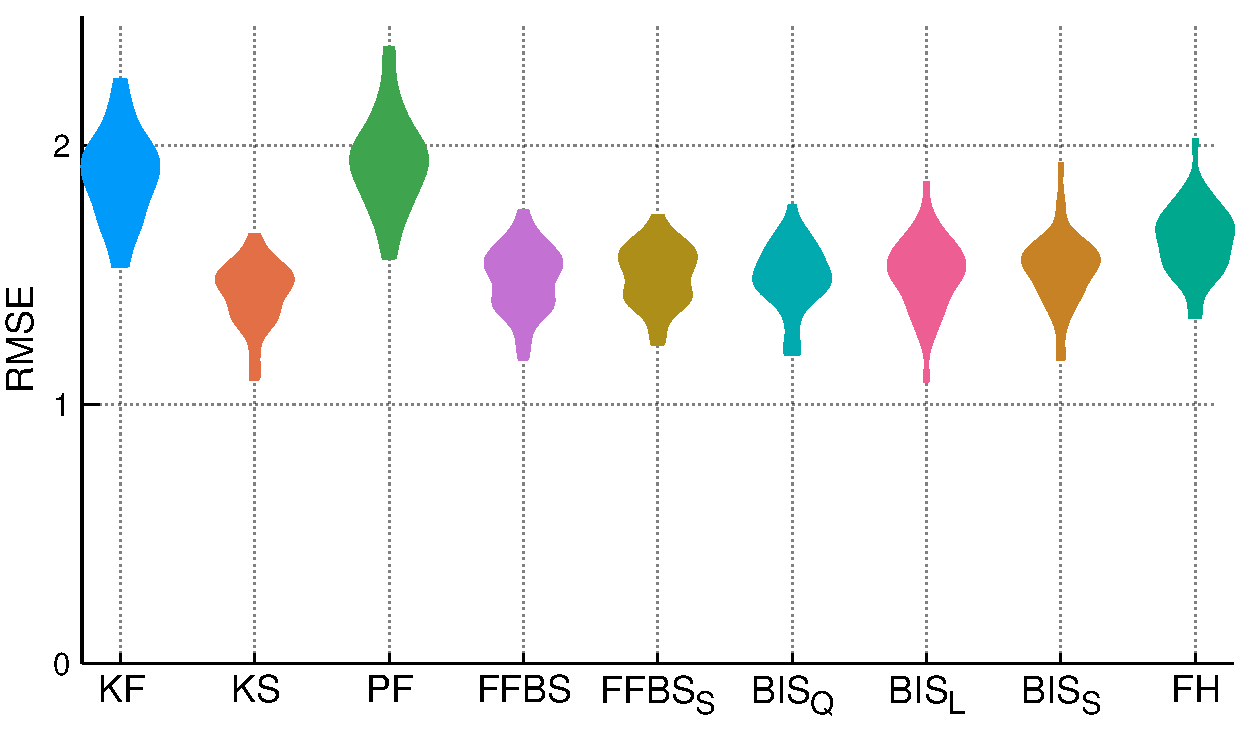
\includegraphics[width=.75\textwidth]{figures/tfs/comparison_caseA}
\caption{\label{comp-smoothing-A}Violin plots comparing the RMSE of the algorithms in \emph{case A} over 50 runs. As expected the optimal Kalman smoother tends to perform best, the FFBS and all BIS have comparable performances while the FH underperforms.}
\end{figure}

\begin{figure}[!h]
\center
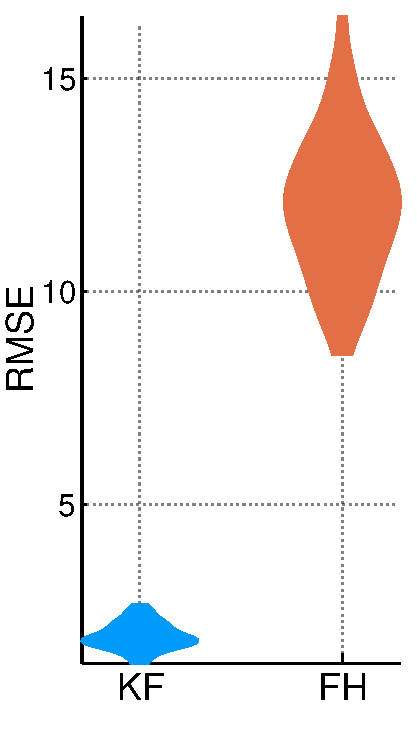
\includegraphics[width=.24\textwidth]{figures/tfs/comparison_caseB_fh+kf}
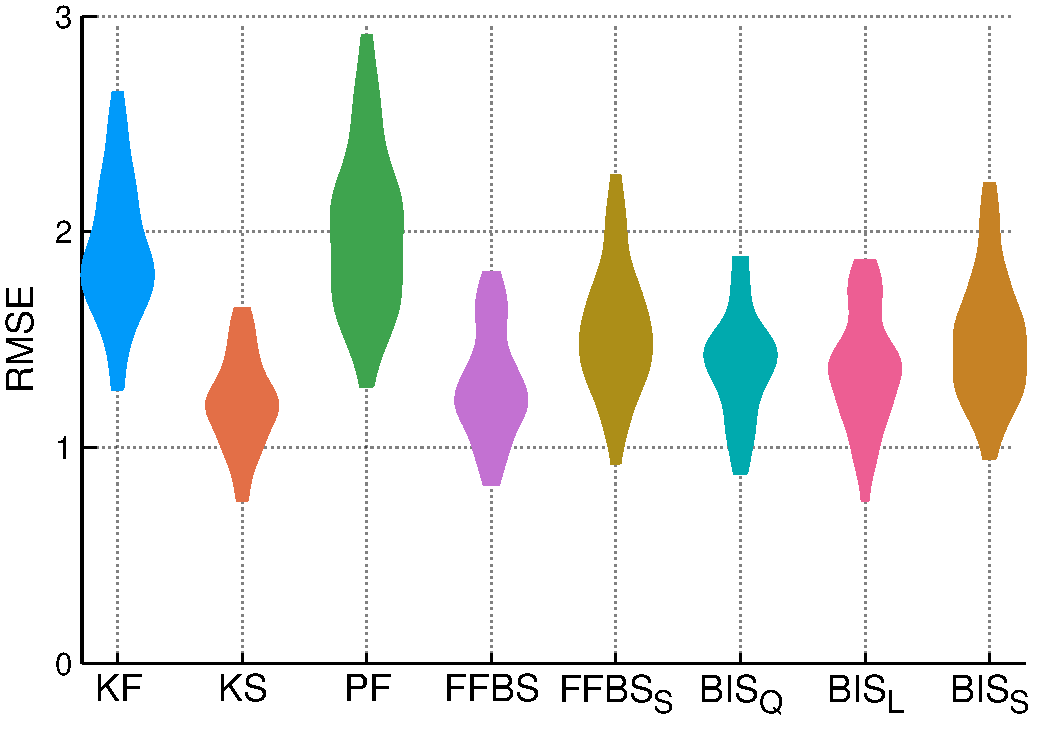
\includegraphics[width=.61\textwidth]{figures/tfs/comparison_caseB}
\caption{\label{comp-smoothing-B}Violin plots comparing the RMSE of the algorithms in \emph{case B} over 50 runs. (left) The FH significantly underperforms  compared to the other algorithms as can be seen compared to the KF which is reproduced on both graph to give an idea of scale (FH is not reproduced on the right as the scale is significantly different from the other algorithms). (right) the other smoothing algorithms offer performances in line with the observations made in case A and do not suffer as much from the decreased noise ratio unlike the FH.}
\end{figure}

%%%%%%%%%%%%%
%\newpage
%%%%%%%%%%%%%

\subsubsection{Model 2 (medium dimensionality)}
In this second example, we consider a model with a 10-dimensional latent space and a 6-dimensional observational space. The matrix $A$ is defined as the identity plus a perturbation matrix $E$ with elements $e_{ij}=\eta_{ij}/5$ with $\eta_{ij}$ drawn from a standard Gaussian. The matrix $B$ has elements $b_{ij}$ drawn from a standard Gaussian. Both matrices $A$ and $B$ are normalised to prevent an explosive behaviour from the HMM. The matrix $Q$ and $R$ have random elements drawn in a similar fashion and both matrices are made positive definite. Both $Q$ and $R$ are normalised and scaled such that $\| Q\| = 1/5$ and $\| R\| = 1/20$. We denote this model LG-10-6 for further reference.

The point of this example is to show that when the particle filter struggles (with a lot of particles with very low weight or, correspondingly, a low ESS) then naturally both version of the FFBS struggle. 
However, the algorithms which apply a resampling of the representation of the particle filter (BIS$_{\text{L}}$ and BIS$_{\text{S}}$) perform very well. Indeed, this resampling allows guiding the smoothing densities to regions of higher expected density (through more concentrated normalising densities $\gamma_{t}$) resulting in better performances overall. The performances are illustrated at figure \ref{comp-model2}.

\begin{figure}[!h]
\center
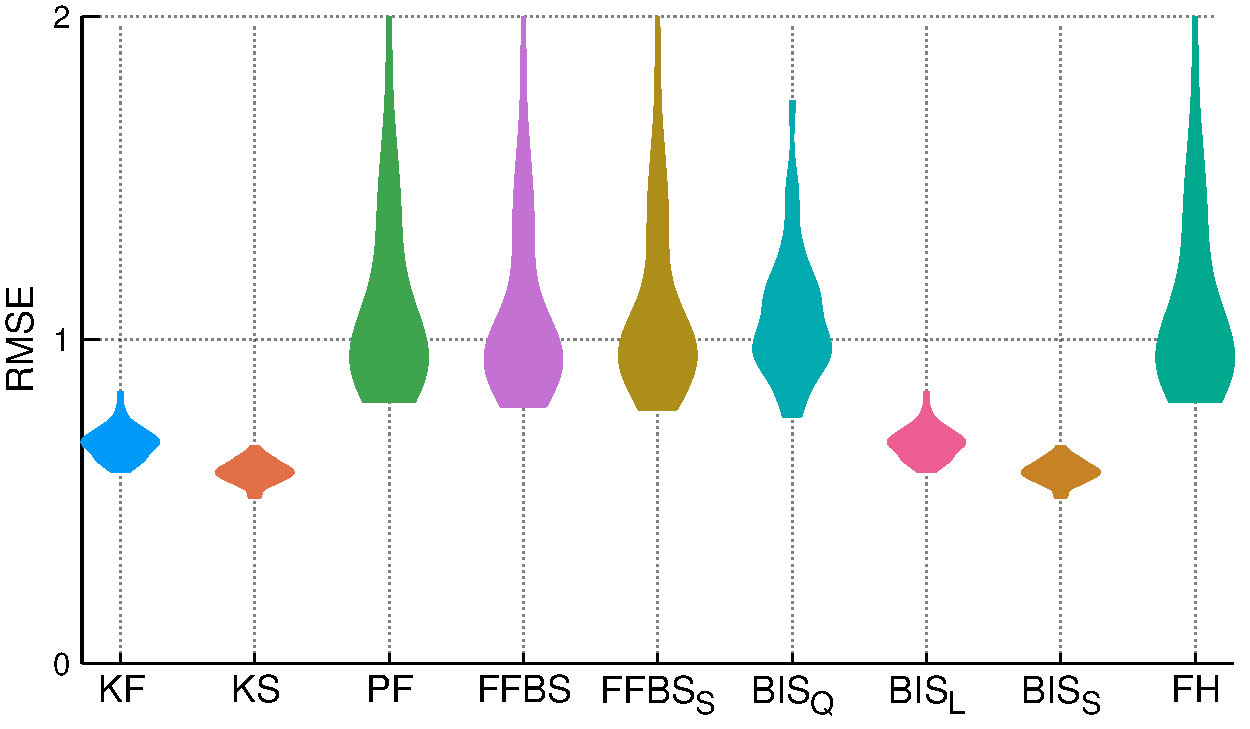
\includegraphics[width=.75\textwidth]{figures/tfs/comparison_mod2}
\caption{\label{comp-model2}Violin plots comparing the RMSE of the algorithms for model LG-10-6 over 50 runs. In this case, the sub-quadratic implementations of the BIS perform outstandingly well compared to the other algorithms which offer little performance gain over simply considering the particle filter.}
\end{figure}

%%%%%%%%
\newpage
%%%%%%%%

\subsection{Nonlinear Gaussian models}
In this point, we show how the sub-quadratic algorithms perform when the dynamic of the HMM is not linear but defined as:
%
\eqa{\syst{ x_{t+1} &=& f_{t}(x_{t}) + \epsilon_{t}\\
		 y_{t+1} &=& g_{t+1}(x_{t+1}) + \eta_{t+1}
}.
}
%
for some sets of functions $\{f_{t}\}_{t=1}^{T}$ and $\{g_{t}\}_{t=1}^{T}$ and with innovation processes $\epsilon_{t}$ and $\eta_{t}$ drawn from centred multivariate Gaussians with covariance matrices $Q$ and $R$.

\subsubsection{Model 3}
This model is drawn from the paper of \citet{arulampalam02} with the dimensionality of both the latent space and the observational space equal to one:
%
\eqa{\syst{
	f_{t}(x) &=& x/2 + 25x(1+x^{2})\inv + 8\cos(1.2t)\\
	g_{t}(x)&=& x^{2}/20\\
},\,\,\text{and}\,\, Q=10,\,\, R=1.
}
%
We call this model NL-1-1 for further reference. We use $N=50$ particles and for $K=100$ time step (as in the original paper) and run the experiments $50$ times with $M=15$ for the sub-quadratic algorithms.

The figure \ref{comp-nl-1} shows the results of the comparison of the RMSE for each algorithm considered. No smoothing algorithm particularly stands out but it shows that the sub-quadratic smoothing algorithms considered do not significantly underperform compared to the full quadratic complexity ones even when the underlying dynamic is non-linear.

\begin{figure}[!h]
\center
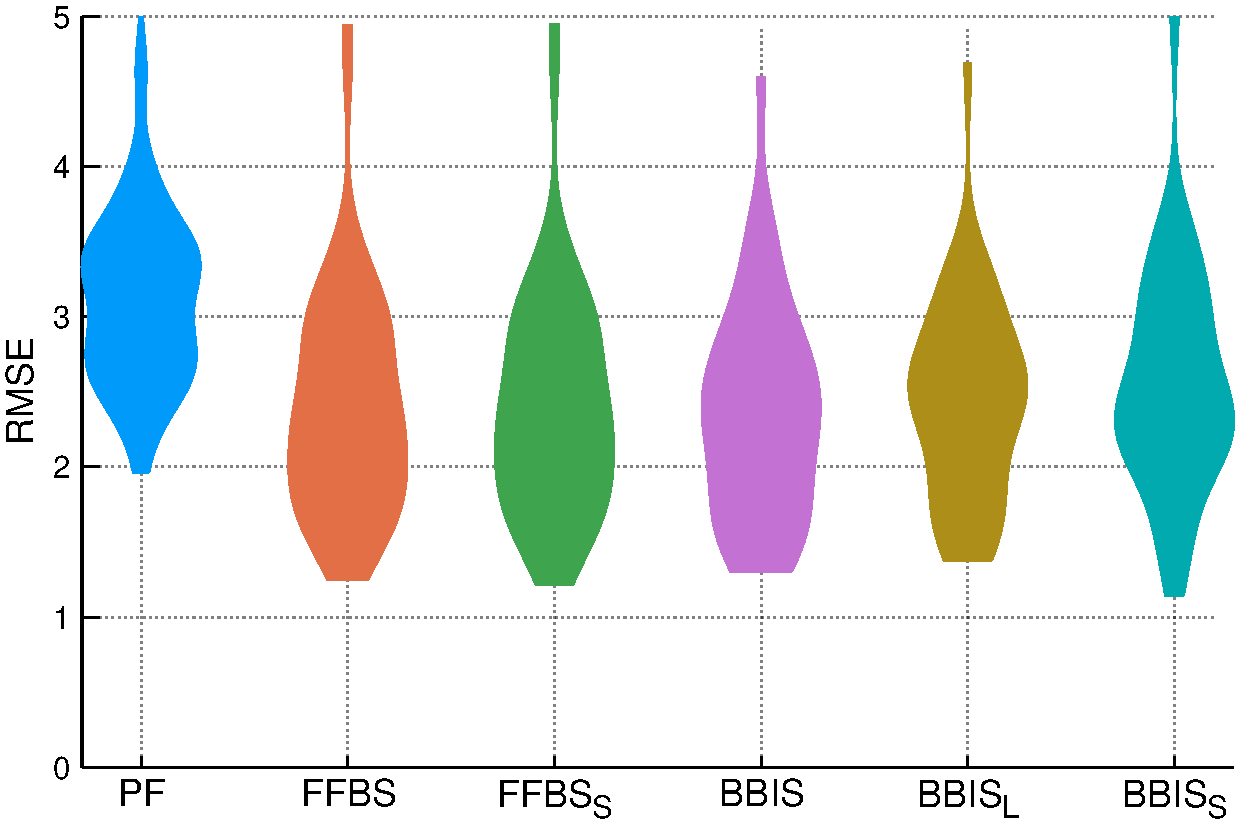
\includegraphics[width=.75\textwidth]{figures/tfs/comp_nl1_N50}
\caption{\label{comp-nl-1}Violin plots comparing the RMSE of the algorithms for model NL-1-1 over 50 runs. In this case, all smoothing algorithms considered offer similar performances showing that sub-quadratic smoothing algorithms can also perform well in the case of a non-linear model.}
\end{figure}

%\subsubsection{Model 4}


\section{Discussion}

In this chapter we suggested and discussed three algorithms with sub-quadratic complexity. 
Two are approximations to the backward information smoother (BIS$_{\text{L}}$, BIS$_{\text{S}}$) using the two filter smoothing algorithm while taking the normalising densities to be approximations of the predictive densities based on a particle filter. 
The last one (FFBS$_{\text{S}}$) is an approximation to the forward filtering backward smoothing algorithm. 

A criticism of the FFBS is that the smoothing step does not sample new particles and just reweighs existing particles which can harm the performance of the resulting estimator. In our experiments however, the FFBS and, more interestingly, its sub-quadratic approximation typically perform well compared to other algorithms. 

The BIS does perform a resampling step in the backward step and uses normalisation densities that are more sensible and typically outperform the default choice suggested in \citep{briers10,fearnhead10}.
However, the optimal backward sampling step is intractable in general and one may have to resort to the bootstrap-BIS as we have in the experiments thereby potentially reducing the advantage of this additional sampling step.

We showed in our experiments that the BIS$_{\text{L}}$ and the BIS$_{\text{S}}$ typically perform on par with the naive implementation. There may be cases in which those algorithms do not perform well but based on the results of the experiments, we would encourage a user to consider the BIS$_{\text{L}}$ as a first smoothing algorithm (provided the dynamic is not linear).

We indicated that the estimators obtained through the BIS$_{\text{L}}$ are not consistent due to the approximation in the sampling of the mixture indices. This, however, seemed to have little impact on the results of the experiments. A possible explanation for this is that, at the regime considered with relatively few particles, all estimators are biased and there is too much variance to significantly distinguish between them. Note however that exploiting these algorithms with significantly more particles (a few orders of magnitude more) requires having to deal with numerical instabilities arising from the representation of the range of weights associated with a large number of particles, and this, even with resampling. This is a known issue, particularly when the dimensionality of the problem is higher and some techniques exist to combat the issue \citep{miguez13}. 

Finally, we have only considered standard multinomial resampling in our algorithms. It may be that alternative resampling procedures such as the ones mentioned in \citet{hol06} lead to improved performances. This could be an avenue for further work.


%Another comment that can be made is that we showed in the previous section that although it was desirable to have $\gamma_{t}\approx \pd_{t}$, it was not necessary as long as $\gamma_{1}=p_{1}$. As shown in \citet{taghavi12}, one could approximate the prediction densities with a mixture of $K$ Gaussians with $K\ll N$ and then consider the full mixture on $KN$ terms instead of a mixture on $N^{2}$ terms. In \citet{taghavi12}, it is shown that mixtures of one or two Gaussians can already provide a good enough approximation to the prediction density in HMM with a simple dynamic. For high-dimensional systems with highly non-Gaussian dynamics however, adjusting a good mixture of a few Gaussians might be expensive and the resulting approximation might be poor.

\fi

%%%%%%%%%%%%%%%%%%%%%%%%%%%%%%%%%%%%%%%
\chapter{Local Bouncy Particle Sampler}

\iflbps% !TEX root = ../thesis.tex

%In this thesis we consider sampling or approximating distributions that factorise in a specific way. 
In this chapter, we cover the Local Bouncy Particle Sampler (LBPS), a version of the BPS introduced in chapter \ref{chap:BGsampling}, section \ref{point:BPS} for target distributions that factorise according to a MRF.

The aim of this short chapter is to show that the LBPS algorithm can be used on high-dimensional models such as probabilistic matrix factorisation and performances are not far those of the HMC algorithm thereby showing the potential of PDMP samplers on complex Machine Learning models. For this, we used our open-source package \texttt{PDSampler.jl} coded in Julia.\footnote{\url{https://github.com/alan-turing-institute/PDSampler.jl}} 

\section{Local Bouncy Particle Sampler}
In \cite{bouchard15}, the authors consider the case where the target distribution factorises as
%
\eqa{
	\pi(x)&\propto& \prod_{f\in F} \gamma_{f}(x_{f})
}
%
where $x_{f}$ is a restriction to a few elements of $x$, $F$ is a set of \emph{factors} and $\gamma_{f}$ is an unnormalised likelihood associated with the factor. In the specific case of a pairwise MRF, the factors are the edges of the graph and the restrictions are the variables corresponding to each nodes. The energy associated to $\pi$ consequently decomposes as $U\equiv \sum_{f\in F}U_{f}$.

%\subsection{Local BPS: algorithm}
For each factor, a local intensity $\lambda_{f}$ and a local bouncing operator $R_{f}$ can be defined in the same way as for the Bouncy Particle Sampler (BPS, see point \ref{point:BPS}) except that $\nabla U_{f}$ is set to have zero components for all variables not associated to the factor. We can then define a collection of intensities with
%
\eqa{
	\chi_{f}(t) &=& \lambda_{f}(x^{(i-1)}+v^{(i-1)}t,v^{(i-1)}). 
}
%
and consider the superposition principle with $\chi\equiv\sum_{f} \chi_{f}$.

Instead of modifying all velocity variables at a bounce as in the basic BPS, the method samples a factor $f$ with probability $\chi_{f}(\tau)/\chi(\tau)$ and modifies only the variables connected to the sampled factor. 
This can significantly reduce the overall computational cost associated with the algorithm and especially so when the underlying MRF has a connection structure that is not too densely connected. Indeed, when an update is triggered at a factor $f$ all factors that share a variable with $f$ are also triggered. If that corresponds to a large portion of the graph, computational gains are lost compared to simply using the full BPS. The algorithm is described in full in \citep[chapter 3.3]{bouchard15}.

%\subsection{Local BPS Algorithm}
%
%\begin{algorithm}[!h]\small
%	\caption{\label{alg:LBPS}\small \idblue{Local BPS with Priority Queue}}
%	\begin{algorithmic}[1]
%	\State initialise $(x^{(0)},v^{(0)})$, set $t_{\text{clock}}=0$
%	\State simulate a first arrival time $\tau_{\text{bounce}}^{f}\sim \text{PP}(\chi_{f}(t))$ for each factor $f$
%	\State initialise a priority queue $Q$ with the couples $\{(\tau_{f}, f)\}_{f\in F}$
%	\State initialise event lists $L_{f}$ for each factor with $(x^{(0)}_{f}, v^{(0)}_{f}, 0)$
%	\State sample $\tau_{\text{ref}}\sim\mathrm{Exp}(\lambda_{\text{ref}})$
%	\While{more events requested}
%		\State pop $(\tau_{f}, f)$ from $Q$ based on the smallest bounce time
%		\If{$\tau_{f}>\tau_{\text{ref}}$} 
%			\State $t_{\text{clock}}\leftarrow t_{\text{clock}}+\tau_{\text{ref}}$
%			\State sample a new $v\sim \mathcal N(0, \mathbb I)$
%			\State start a new queue $Q$ where the positions for each factor is extrapolated linearly until the refreshment time
%		\Else
%			\State $t_{\text{clock}}\leftarrow t_{\text{clock}}+\tau_{f}$
%			\State extrapolate $x_{f}$ linearly until $t_{\text{clock}}$
%			\State 
%		\EndIf
%	\EndWhile
%	\end{algorithmic}
%\end{algorithm}



\section{Probabilistic Matrix Factorisation}

Probabilistic Matrix Factorisation (PMF) \citep{mnih08} is a Bayesian approach to the matrix completion problem. In that problem, we consider a matrix $R$ of size $n\times p$ of ratings $r_{ij}$ corresponding to user $i$ and item $j$ (e.g.: a movie) but we only have access to a mask of $R$, a very sparse subset of the ratings which we denote $\hat R$. The aim of matrix completion methods such as PMF is to try to construct a low-rank factorisation  $R\approx U^{t}V$ based on the known entries where $U$ is of size $d\times n$ and $V$ of size $n\times p$ and $d$ is very small compared to $n$ or $p$. 

\subsection{Description of the  Model}

The model described in \citep{mnih08} assumes that each rating $r_{ij}$ is a realisation from a Normal random variable with mean $\scal{u_{i}, v_{j}}$ and standard deviation $\sigma_{r}$. 
Further, the model assumes spherical Gaussian priors on all $u_{i}$ and $v_{j}$ with standard deviation $\sigma_{u}$ and $\sigma_{v}$ respectively. Formally:
%
\begin{eqnarray}
	r_{ij} &\sim& \mathcal N(\,\cdot\, ; \scal{u_{i}, v_{j}}, \sigma_{r}), \qquad (i,j)\in\mathcal M\nn\\
	u_{i} &\sim& \mathcal N(\,\cdot\, ; 0_{d}, \sigma_{u}\mathbb I_{d}), \qquad i\in 1,\dots,n \label{eq:pmf-model}\\
	v_{j} &\sim& \mathcal N(\,\cdot\, ; 0_{d}, \sigma_{v}\mathbb I_{d}), \qquad j\in 1,\dots,p\nn
\end{eqnarray}
%
where $\mathcal M$ denotes the entries which are available, $0_{d}$ and $\mathbb I_{d}$ denote the zero vector in $\mathbb R^{d}$ and the $d\times d$ identity matrix respectively. In our experiments, we assume $\sigma_{r}, \sigma_{u}$ and $\sigma_{v}$ are fixed,\footnote{In practice, we compute sensible estimates from the data following the authors' original code available at \url{http://www.cs.toronto.edu/~rsalakhu/BPMF.html}.} more involved models exist including hyper-priors which we will not consider here since our aim is primarily to compare Local BPS and HMC on a large scale model rather than produce the best performing PMF method.\footnote{In \citep{mnih08} also suggest doing a few steps of Gibbs sampling for the hyperparameters. We do not do this in order to simplify the computations and the comparisons.}

Finally, note that the full dimensionality of the model is $n\times d + p\times d$. Below we consider an example where $d=10$, $n=6000$, $p=4000$ and $|\mathcal M|=10^{6}$ meaning that the full dimensionality of the model is $100 000$ with 1 million factors. For that kind of scale, a method such as naive Gibbs sampling (see point \ref{point:classical-sampling}) is impractical. 


\subsection{Local BPS for the PMF}

The factor graph corresponding to the matrix factorisation problem has a simple structure: each rating $r_{ij}$ for $(i,j)\in\mathcal M$ corresponds to a factor connected to the variables $u_{i}$ and $v_{j}$. This is illustrated at the figure \ref{fig:pmf-graph} below.

\begin{figure}[!h]
\center
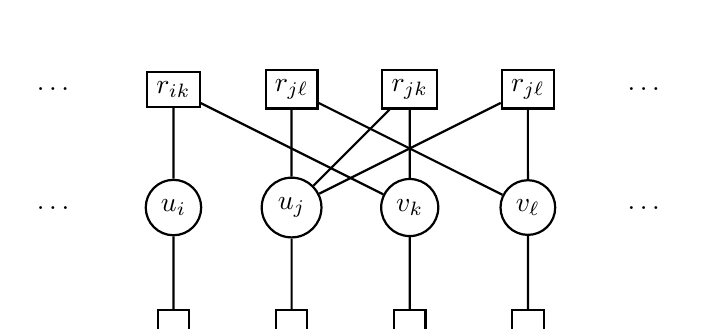
\begin{tikzpicture}[-,minimum size=.4cm,scale=.1,node distance=1.5cm, thick]
	\node[]				(A0)				{$\dots$};
	\node[rectangle,draw]	(A) [right of=A0]	{$r_{ik}$};
	\node[rectangle,draw] 	(B) [right of=A]		{$r_{j\ell}$};
	\node[rectangle,draw]	(C) [right of=B]		{$r_{jk}$};
	\node[rectangle,draw]	(E) [right of=C]		{$r_{j\ell}$};
	\node[] 				(D) [right of=E]  	{$\dots$};
	\node[circle,draw] 		(F1) [below of=A] 	{$u_{i}$};
	\node[circle,draw] 		(F2) [below of=B] 	{$u_{j}$};
	\node[circle,draw] 		(F3) [below of=C] 	{$v_{k}$};
	\node[circle,draw] 		(F4) [below of=E] 	{$v_{\ell}$};
	\node[] 				(F5) [right of=F4] 	{$\dots$};
	\node[]				(F6) [left of=F1]		{$\dots$};
	\node[rectangle,draw]	(G1)[below of=F1] 	{};
	\node[rectangle,draw]	(G2)[below of=F2] 	{};
	\node[rectangle,draw]	(G3)[below of=F3] 	{};
	\node[rectangle,draw]	(G4)[below of=F4] 	{};
	\path 
	(A) edge	(F1)
	(A) edge	(F3)
	(B) edge	(F2)
	(B) edge 	(F4)
	(C) edge 	(F2)
	(C) edge 	(F3)
	(E) edge 	(F2)
	(E) edge	(F4)
	(G1) edge (F1)
	(G2) edge (F2)
	(G3) edge (F3)
	(G4) edge (F4)
	;
\end{tikzpicture}
\caption{\label{fig:pmf-graph} Illustration of the factor-graph corresponding to the matrix completion problem. Each observed rating corresponds to a factor connected to a corresponding $u$-node and $v$-node themselves corresponding to $d$-dimensional variables. Each node also has its own factor corresponding to a spherical Gaussian prior (empty squares).}
\end{figure} 

% Note that while every rating factor has degree 2 in the graph whereas it can vary for each variable nodes.  

The energy associated with one of the rating factor is also easily obtained by taking the negative log-likelihood associated to $r_{ij}$ (see \eqref{eq:pmf-model}), we denote it $\mathcal E_{ij}$ with
%
\eqa{
	\mathcal E_{ij}(u_{i}, v_{j}) &:=& 0.5\sigma_{r}^{-2}(r_{ij}-\scal{u_{i}, v_{j}})^{2}.
}
%
Correspondingly, the prior-factors are associated with $\mathcal E^{u}_{i}(u_{i}):=0.5\sigma_{u}^{-2}\|u_{i}\|_{2}^{2}$ and $\mathcal E^{v}_{j}(v_{j}):=0.5\sigma_{v}^{-2}\|v_{j}\|_{2}^{2}$. The Inhomogeneous Poisson Processes (IPP) associated with Gaussians can easily be sampled from using the inversion method. 
The IPP associated with the rating factors can also be easily sampled from using the inversion method which we show below.

\subsubsection{Sampling the IPP associated with a rating factor}

To simplify notations, we consider a single rating $r$ associated with two $d$-dimensional vectors $u$ and $v$. We introduce the notation $x:=(u; v)$ and write $x_{u}=u$ and $x_{v}=v$. We also write $e(x):=(\scal{x_{u},x_{v}}-r)$. With these notations, we can write the energy as $\mathcal E(x) = 0.5\sigma_{r}^{-2}e^{2}(x)$. 
As for the BPS, the intensity associated with this factor is $\chi(t) = \scal{\nabla \mathcal E(x+tw), w}^{+}$ where $w$ is a velocity-vector of the same dimension as $x$. The gradient with respect to the $u$ and $v$ component can be written as
\eqa{
	\syst{\nabla_{x_{u}} \mathcal E(x) &=& \gamma(x)x_{v}\\
		\nabla_{x_{v}} \mathcal E(x) &=& \gamma(x)x_{u}}
}
where $\gamma(x):=\sigma_{r}^{-2}e(x)$. It is straightforward to show that the inner product \\$\scal{\nabla\mathcal E(x+tw), w}$ is a third-order polynomial in $t$ with
\eqa{
	\scal{\nabla\mathcal E(x+tw), w} &=& \gamma(x+tw)\pac{\scal{x_{u},w_{v}} + \scal{x_{v}, w_{u}} + 2t\scal{w_{u}, w_{v}}} \label{ipp-3dorder}
}
The intensity $\chi(t)$ of the IPP is therefore given by the positive part of this third-order polynomial. The factor of $t^{3}$ in \eqref{ipp-3dorder} is positive which is already indicative of the shape of the polynomial but the roots of the polynomial need to be studied in order to fully characterise it. It is easy to obtain the root corresponding to the left-parenthesis in \eqref{ipp-3dorder} which we denote $t_{0}$ with $t_{0}=-d(x,w)/2s(w)$ where $d(x,w):=(\scal{x_{u}, w_{v}}+\scal{x_{v},w_{u}})$ and $s(w):=\scal{w_{u},w_{v}}$. The other two roots are obtained by setting $\gamma(x+tw)$ or equivalently $e(x+tw)$ to zero. All the roots of \eqref{ipp-3dorder} are therefore given by:
\eqa{
	\syst{	t_{0} &=& -d(x,w)/2s(w)\\
			t_{-,+} &=& t_{0} \pm \sqrt{t_{0}^{2}+e(x)/s(w)}	}.
}

Using the inversion method, sampling from the IPP can be done in two steps: generate a $\lambda\sim\mathrm{Exp}(1)$ and then find $t(\lambda)$ such that
\eqa{
	\lambda \spe \Xi(t(\lambda)) &=& \int_{0}^{t(\lambda)} \chi(s)\ds.
}
Since $\chi(t)$ is the positive part of a third-order polynomial, the integral can be computed exactly and the inversion to obtain $t(\lambda)$ amounts to finding a root of a fourth-order polynomial which can be done efficiently using a numerical solver. 

%\mathcal{}


\subsection{Other algorithms considered}

\subsubsection{Singular Value Decomposition}

As a baseline, we consider the Singular Value Decomposition (SVD) algorithm. Indeed, Eckart and Young's theorem shows that for a matrix $M$, the truncated SVD is the best low-rank approximation in the sense of the Frobenius norm. In the matrix completion case, no guarantees are offered by the SVD since we only have access to a sparse mask of the real matrix \citep{srebro04}. Let $R$ denote the true matrix we are trying to reconstruct and $\hat R$ the sparse matrix containing only the observed ratings (centred). The SVD decomposition of $\hat R$ gives $\hat R = U\Sigma V^{t}$ where $U$ is an orthonormal matrix of size $n\times p$, $\Sigma$ is a diagonal matrix of size $p\times p$ and $V$ is an orthogonal matrix of size $p\times p$. Truncating $\Sigma$ to its first $d\ll p$ components leads to a rank-$d$ approximation $\tilde R$ to $\hat R$. 
Letting $U_{\text{SVD}}:=\Sigma^{1/2}U^{t}$ and $V_{\text{SVD}}:=\Sigma^{1/2}V^{t}$ we have a first baseline factorisation $\tilde R=U_{\text{SVD}}^{t}V_{\text{SVD}}\approx R$.

Note that the problem of computing a truncated SVD decomposition of a large sparse system is a well known problem in numerical linear algebra and very efficient methods exist \citep{sorensen96}.\footnote{In the experiments, we use the \texttt{svds} function from Julia 0.6 uses the implicitly restarted Lanczos iterations.} 

\subsubsection{Hamiltonian Monte Carlo}

The negative log posterior in $U$ and $V$ of the model can be directly obtained:
\eqa{
	-2\log p (U, V | \hat R) &=& \sigma_{r}^{-2}\sum_{(i,j)\in\mathcal M} (r_{ij}-\scal{u_{i},v_{j}})^{2} +\sigma_{u}^{-2}\|U\|_{2}^{2} + \sigma_{v}^{-2}\|V\|_{2}^{2}.\nn
}
Therefore, the gradient in $u_{i}$ and $v_{j}$ can easily be computed in closed form and it is straightforward to apply HMC on this model (cf.\ algorithm \ref{alg:hmc-alg}). The main hurdle is that each gradient evaluation requires a full pass over all observed ratings making iterations expensive. 

\subsection{Experiments}

In our experiments, we consider the MovieLens 1M dataset.\footnote{\url{https://grouplens.org/datasets/movielens/}} corresponding to 1 million ratings of 4000 movies by 6000 users. We take a random subset of 95\% of the ratings as training set using the remaining 5\% as test set. 
Following the literature, we use $d=30$; we set $\sigma_{R}=1$ and $\sigma_{U}=\sigma_{V}=10$. The starting point is drawn from a standard multivariate Normal centred at the solution of the SVD algorithm. The Local BPS experiments use the \texttt{PDSampler.jl} package, the HMC simulations use 2 leapfrog steps, the stepsize is set to $0.01$. The reported value is the RMSE over the test set. We run each experiments ten times to account for the stochasticity of the algorithms. All results were obtained using Julia 0.6 with a 2.3GHz Intel Core i5 computer. 

\newpage
\begin{figure}
	\center
	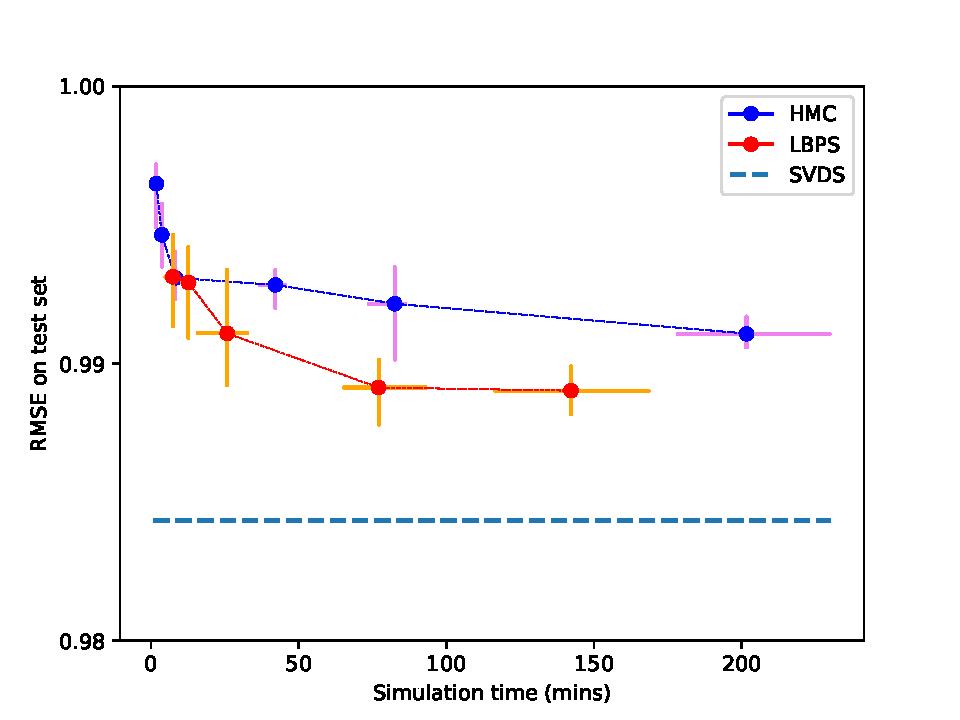
\includegraphics[width=.8\textwidth]{figures/lbp/curves}
	\caption{\label{fig:LBPSvHMC}RMSE on the test set of the MovieLens 1M dataset when using Probabilistic Matrix Factorisation with HMC and the LBPS algorithm compared to the result obtained with the Sparse SVD algorithm. The crosses indicate the range of values obtained and ranges of times for each of the 10 runs recorded for different simulation lengths. The dashed lines connects the means.}
\end{figure}

The results displayed on the figure \ref{fig:LBPSvHMC} seem to show that the LBPS does a little bit better in this case than the HMC algorithm. The improvement is not very significant but confirms that the BPS and the LBPS can perform as well or better than the HMC algorithm (a similar result had been obtained by \citep{bouchard15} on a much simpler factor graph). 

Both methods underperform significantly compared to the test-RMSE obtained with the sparse SVD.  This may be a poor choice of hyper parameters though after trying a range of possible hyper parameters we did not see major differences. In this case it may just be that the SVDS algorithm performs very well and does not overfit the data rendering the regularisation that appears in the PMF model useless. 

\section{Discussion}

The main purpose of this chapter was to compare the HMC algorithm to the LBPS on a very high-dimensional model with a rather sparse graphical model structure. We showed in the experiments that the LBPS compares favourably with HMC in this case which gives hope for future use of the LBPS on large scale graphical models.

Much remains to be explored on how to better tune Piecewise Deterministic samplers and in particular on graphical models. To the best of our knowledge, this was the first attempt to use the LBPS on a large-scale model in statistics or machine learning. 

\begin{figure}[!h]
\center
	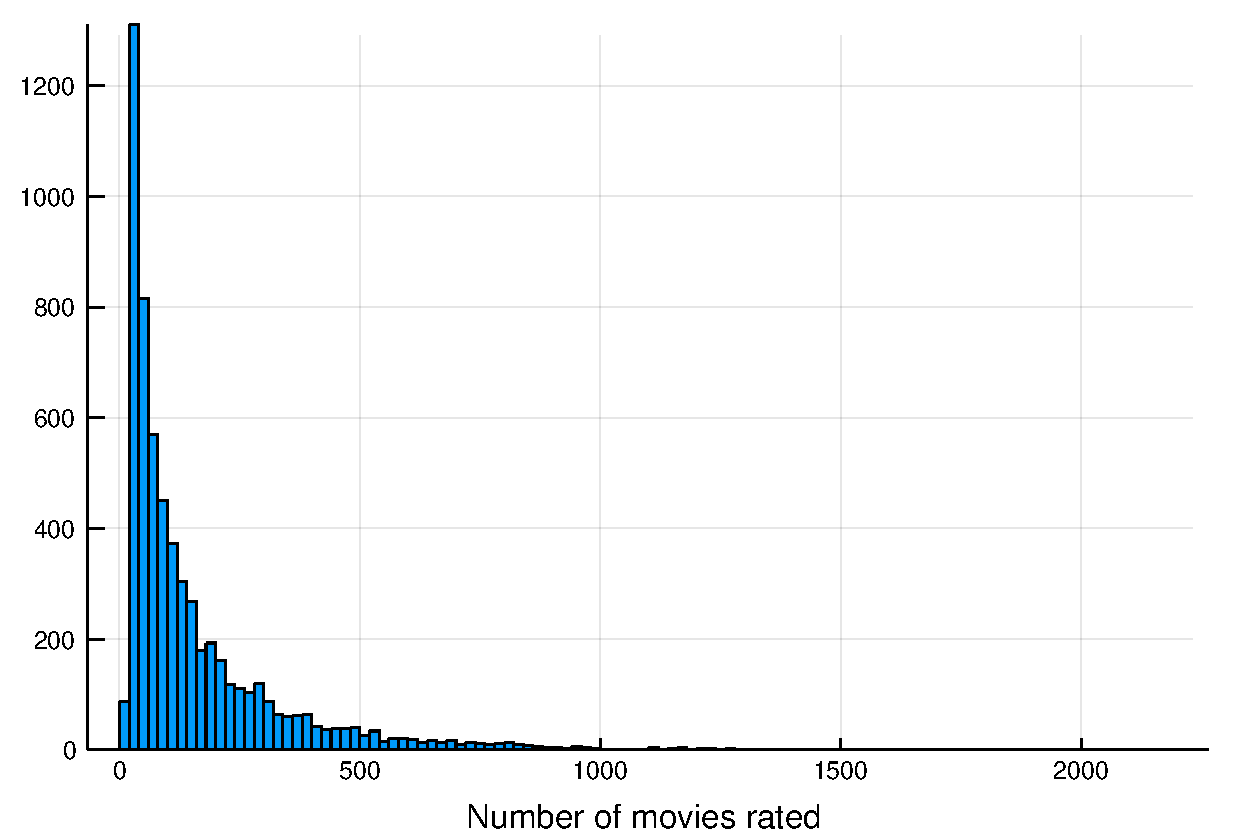
\includegraphics[width=.7\textwidth]{figures/lbp/hist}
	\caption{\label{fig:nratings}Histogram of the number of ratings per users.}
\end{figure}

A key element for the viability of the LBPS for a large scale graphical model is the sparsity of the graph. As we hinted at earlier, if each variable node is connected to many factors then every time a factor is triggered, every factor that shares a variable with it is also triggered. If this is a large portion of the graph, the advantage of exploiting the factorisation structure of the model is severely diminished. 
In the figure \ref{fig:nratings}, we look at the distribution of the number of ratings per users. It shows that the distribution is heavy tailed with a significant number of users having over 250 ratings (1149 users). This along with the slow convergence we observed for the LBPS in figure \ref{fig:LBPSvHMC} suggests that the LBPS may be struggling due to the graph not being sparse enough.

Future work could look at other models which offer a sparse conditional dependence structure and compare the LBPS with the BPS. We suspect that for very sparse models the LBPS will outperform the BPS as observed experimentally for Gaussian Random Fields in \citep{bouchard15}. %but it is unclear at which point the BPS starts outperforming the LBPS. 



\fi

%%%%%%%%%%%%%%%%%%%%%%%%%%%%%%%%%
% SECOND PART -------------------
%%%%%%%%%%%%%%%%%%%%%%%%%%%%%%%%%
\part{Variational Inference} % part II

%%%%%%%%%%%%%%%%%%%%
\chapter{Background}

\ifbgm% !TEX root = ../thesis.tex

%%%%%%%%%%%%%%%%%%%%%%%%%%%%%%%
\section{Overview of Approximate Bayesian Inference}

% !TEX root = ../thesis.tex

In this thesis we define approximate Bayesian inference in broad terms as the class of methods attempting to recover a distribution $q$ in a restricted family of distributions $\mathcal F\subset \mathcal P(\mathcal X)$ such that $q$ is a ``good'' proxy for a posterior distribution $p$ of interest. 
This definition leaves significant room to describe different methods based on the definition of what a good proxy means. 

Let $D:\mathcal P(\mathcal X)\times \mathcal P(\mathcal X)\to \mathbb R_{+}$ denote a discrepancy measure between two probability distribution functions. Then, the generic variational problem we consider is the minimisation of this discrepancy in $\mathcal F$:
%
\eqa{
q^{\star} &\in& \arg\min_{q\in \mathcal F}\quad D(q,p).\label{eq:generic-abi}
}
%
Techniques attempting to solve such problems rely upon exploiting at least one of the three main characteristics: the definition of the discrepancy measure $D$, the definition of the restricted space $\mathcal F$ and the structure of the target distribution $p$. 

Many discrepancy measures can be considered such as the total variation distance, the Wasserstein distance or $f$-divergences \citep{minka04, blei16, li16, bernton17}. However, most choices lead to the corresponding problem \eqref{eq:generic-abi} being computationally very expensive to solve in general especially when the space $\mathcal X$ is continuous.
%%%%%%%%%%%%%%%%%
\subsection{Variational inference}
A popular discrepancy measure that has been widely considered in the literature partly because it leads to variational problems that can be solved cheaply is the Kullback-Leibler divergence. Considering the discrepancy $\KL{q,p}$ leads to the popular \emph{variational inference} algorithms \citep{blei16}. 


In \emph{mean-field variational inference} (MFVI), $\mathcal F$ is taken to be the class of distributions that fully factorises:
%
\eqa{
	\mathcal F_{\text{VI}} &=& \pab{q \in \mathcal P(\mathcal X) \st q(x_{1},\dots,x_{d}) = \prod_{i=1}^{d}q_{i}(x_{i}) }.
}
% 
This choice of distribution space, while rather restrictive, leads to the inference problem \eqref{eq:generic-abi} being tractable and efficient iterative schemes based on the gradient descent can be used that provably decrease the objective function \citep{hoffman13, kucukelbir16, blei16}. However, the problem is non-convex and no guarantees exist as to what these methods converge to.\add{in discussion, the graph with things to explain where converges to}\add{maybe clarify why discussed here and then not used in rest --> EP, LBP take more advantage of structure of target}

\subsection{Other methods}

The Assumed Density Filtering (ADF) algorithm and the  Expectation Propagation (EP) algorithm are two other popular methods that are also based on the KL divergence (albeit the reversed one, see point \ref{s:ADF+EP}).
The choice of distribution space is usually the exponential family associated with a sufficient statistic $\phi$ (see point \ref{point:expof-convex}). Additionally, these methods assume that the target distribution $p$ factorises in terms that are easier to handle than $p$ itself (see point \ref{s:ADF+EP}).

The Belief Propagation (BP) algorithm and the Loopy Belief Propagation (LBP) algorithm are message-passing algorithms which target distributions that factorise according to a MRF. Those methods can also be shown to be fixed-point algorithms corresponding to a specific form of \eqref{eq:generic-abi} \citep{yedidia01, yedidia02}.

In this part of the thesis we focus on the use of EP and (L)BP algorithms for inference on MRF and discuss applications. In point \ref{s:ADF+EP} we cover the ADF and EP algorithms with exponential family distributions and in point \ref{bg:belief-propag} we introduce the BP and LBP algorithms.






%%%%%%%%%%%%%%%%%%%%%%%%%%%%%%%%%
\section{Expectation Propagation}
% ===============================================
\newpage
\subsection{\label{point:expof-convex}The exponential family and convexity}

% !TEX root = ../thesis.tex

\todofr{
\begin{itemize}
	\item General reference, say that aim is to be self contained rather than completely general, suggest Brown and Rockafellar for the details.
	\item notations inspired from \citet{wainwright08}
\end{itemize}
}

\subsubsection*{Log partition function and natural parameter space
}
%Following \citet{wainwright08} 
We define the \emph{exponential family} $\mathcal F_\phi(\mathcal X)\subseteq\mathcal P(\mathcal X)$ associated with a sufficient statistic $\phi:\mathcal X\to\R^{d}$ on a set $\mathcal X\subseteq \R^{n}$ as the collection of probability distribution functions indexed by a parameter $\theta\in\R^{d}$ and of the form\add{review notations, stick to theta for approximating density}
%
\eqa{
	q_\theta(x)&=& \exp\pat{\scal{\theta,\phi(x)}-A(\theta)}
}
%
with respect to a base measure $\nu$ on $\mathcal X$. The \emph{log partition} function $A$ is defined such as to normalise $q_{\theta}$:
%
\eqa{
	A(\theta) &=& \log \int_{\mathcal X} \exp\scal{\theta,\phi(x)}\nudx
.
}
%
The set of \emph{natural parameters} $\Omega \subseteq \mathbb R^{d}$ is defined as the set of parameters $\theta$ such that $A(\theta)$ is bounded (and, therefore, $q_\theta$ is a proper distribution):\check{may15, april16}
\eqa{	\Omega &:=& \{\theta\in\R^{d}\mid A(\theta) \,<\,\infty\}.\label{def:natural} 	}
%
An exponential family is said to be \emph{regular}\margnote{regular fam.} when the corresponding set $\Omega$ is nonempty and open. Additionally, an exponential family is said to be \emph{minimal}\margnote{minimal fam.} provided there does not exist a nonzero vector $a\in\mathbb R^{d}$ such that $\scal{a,\phi(x)}$ is constant $\nu$-almost everywhere. A distribution in a minimal exponential family is therefore one-to-one with its parameter $\theta\in\Omega$. In the rest of this document, we will assume that we are working with a regular and minimal exponential family unless otherwise mentioned.\add{check, add comment otherwise}\check{may15, april16}

The log-partition function $A$ is convex on $\Omega$. Indeed, let $\theta_1,\theta_2\in\Omega$ and $\lambda\in[0,1]$, then using H\"older's inequality with parameters $(1-\lambda)\inv$ and $\lambda\inv$, we can write:\footnote{For two real-valued measurable functions $f$ and $g$, H\"older's inequality with parameters $p,q\in[1,\infty]$ states that $\|fg\|_{1}\le \|f\|_{p}\|g\|_{q}$ provided $p\inv+q\inv=1$.}
\eqa{
	\int \exp\scal{(1-\lambda)\theta_1,\phi(x)}\exp\scal{\lambda\theta_2,\phi(x)}\nudx\hspace*{-2cm}&&\nn\\
	 &\le& \exp(A(\theta_1))^{1-\lambda} \exp(A(\theta_2))^{\lambda}.\label{eq:holderlogp}
}
Taking the logarithm of that inequality shows that $A$ is convex on $\Omega$ and therefore that $\Omega$ itself is convex.\check{may15, april16}\add{Actually $\Omega$ is the \emph{effective domain} of $A$, Rockafellar p.23}
%
\subsubsection*{Gradient and convex-conjugate of $A$}
In a regular exponential family, it is well known \citep[theorem 2.2]{brown86} that the log-partition function is infinitely continuously differentiable and that its gradient and Hessian are related to the first two moments of the sufficient statistic:\add{make sure the notations are clarified somewhere}
%
\eqa{
	\nabla A(\theta) &=& \E_{q_\theta}[\phi(X)] \nn\\
	\nabla^{2}	A(\theta) &=& \mathbb V_{q_\theta}[\phi(X)].\nn
}
%
An important consequence is that, for a minimal exponential family, the covariance matrix $\V_{q_\theta}[\phi(X)]$ is positive definite which in turns implies that $A$ is strictly convex on $\Omega$. Indeed, take any nonzero vector $a\in\mathbb R^{d}$ then by definition, $\scal{a,\phi(X)}$ cannot be constant $\nu$-almost everywhere so that $\mathbb V_{q_{\theta}}[\scal{a,\phi(X)}] > 0$ for any $\theta\in\Omega$ and therefore:
\eqa{	0 &<& \scal{a ,\mathbb V_{q_{\theta}}[\phi(X)] a}, 	}
so that $\mathbb V_{q_{\theta}}[\phi(X)]$ is positive definite.\check{may15, april 16} 
Let $\mathcal M^{\star}$ denote the image of $\Omega$ under the gradient mapping $\nabla A$ or $\mathcal M^{\star}=\nabla A(\Omega)$. Since $A$ is strictly convex, $\nabla A$ is a strictly monotone map, and it forms a bijection between $\Omega$ and $\mathcal M^{\star}$. Let $\theta^{\star}$ be the image of a point $\mu^{\star}\in\mathcal M^{\star}$ through the inverse map $(\nabla A)\inv$. 
This can be written as
%
\eqa{
	\theta^{\star} &=& \{ \theta\in\Omega \mid \nabla A(\theta)=\mu^{\star}\},\nn\\
	&=& \{ \theta\in\Omega\mid \nabla(A(\theta)-\scal{\theta,\mu^{\star}})=0\}.
}
%
Since $A(\theta)-\scal{\theta,\mu}$ is a strictly convex function in $\theta$, this corresponds to a first-order condition for its minimiser.
\footnote{A first-order condition for a minimiser indicates that for a convex, differentiable function $f$ on a set $\Omega$, $\{x\in\Omega\mid \nabla f(x)=0 \}\subseteq\arg\min_{x}\,\,f(x)$. If there exists a unique point $x^{\star}\in\Omega$ such that $\nabla f(x^{\star})=0$ then it is also the unique minimiser of $f$ and both sets are equal to that point \citep[theorem 27.1]{rockafellar70}. } Therefore, we can write\check{may15, april16}
%
\eqa{
	\theta^{\star} &=& \arg\min_{\theta\in\Omega} \quad A(\theta)-\scal{\theta,\mu^{\star}}
}
%
which is related to the convex-conjugate of $A$ on $\mathcal M^{\star}$ defined as
\eqa{
	A^{\star}(\mu) &:=& \max_{\theta\in\Omega}\quad \scal{\theta,\mu} - A(\theta).\label{eq:defconja}
}
Note that $A^{\star}$ is itself a convex function \citep[Theorem 12.2]{rockafellar70}. Using this definition, we have
%
\eqa{	
	A^{\star}(\mu^{\star}) &=& \scal{\theta^{\star},\mu^{\star}}-A(\theta^{\star})	\label{eq:duality1}
}
%
and $(\theta^{\star},\mu^{\star})$ is said to form a \emph{dual pair}. Let us now consider an arbitrary $\theta^{+}\in\Omega\backslash\{\theta^{\star}\}$ and the corresponding $\mu^{+}=\nabla A(\theta^{+})\in\mathcal M^{\star}$. Then, by strict convexity of $A$, we have\check{may15, april17}
%
\eqa{	
	A(\theta^{\star}) &>& A(\theta^{+}) + \scal{\theta^{\star}-\theta^{+},\mu^{+}}.	
	}
%
Using the duality property \eqref{eq:duality1} and with $\mu^{\star}=\nabla A(\theta^{\star})$, the previous inequality reads
%
\eqa{	
	-A^{\star}(\mu^{\star}) + \scal{\theta^{\star},\mu^{\star}} &>& -A^{\star}(\mu^{+})+\scal{\theta^{+},\mu^{+}} + \scal{\theta^{\star}-\theta^{+},\mu^{+}}.\nn\\
	\Longleftrightarrow	\quad A^{\star}(\mu^{+}) &>& A^{\star}(\mu^{\star}) + \scal{\mu^{+}-\mu^{\star},\theta^{\star}}.\label{eq:dualprop}
	}
%
Since the inequality \eqref{eq:dualprop} holds for any $\mu^{+}\neq \mu^{\star}$, $\theta^{\star}$ is said to be a \emph{subgradient} of $A^{\star}$ at $\mu^{\star}$. Since the mapping $\nabla A$ is one-to-one on $\Omega$, $\theta^{\star}$ is necessarily the only such subgradient. Therefore, $A^{\star}$ is differentiable on $\mathcal M$ \citep[theorem 25.1]{rockafellar70} and $\nabla A^{\star}$ is the inverse mapping of $(\nabla A)\inv$ from $\mathcal M^{\star}$ to $\Omega$. The relationship is illustrated at the \fig{bijOmM} below.\check{may15}

\begin{figure}[!h]
	\center
	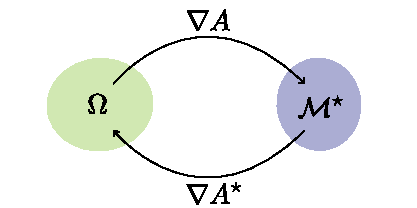
\includegraphics{figures/expf/mapping}
	\caption{\label{bijOmM}Illustration of the bijection between the set of natural parameters $\Omega$ and its image under $\nabla A$, $\mathcal M^{\star}$.}
\end{figure}
%
\subsubsection*{Mean parameter space}
It remains to characterise more precisely the set $\mathcal M^{\star}=\nabla A(\Omega)$. It is a subset of the set of realisable \emph{mean parameters}:
%
\eqa{
	\mathcal M^{\star} \esp\subseteq\esp \mathcal M &:=& \pab{\mu\in\mathbb R^{d}\mid \exists\, p \in\mathcal P(\mathcal X) \,\,\text{s.t.}\,\, \mu=\E_{p}[\phi(X)] },
}
%
where $\mathcal P(\mathcal X)$ denotes the set of all probability density functions on $\mathcal X$. This space $\mathcal M$ is also known as the \emph{mean parameter space}. It is easy to see that it is convex since $\mathcal P(\mathcal X)$ is convex. More interestingly, it can be shown that, for a minimal exponential family, $\mathcal M^{\star}$ is, in fact, the interior of $\mathcal M$ \citep[theorem 3.3]{wainwright08}. Note that, since the interior of a convex set is necessarily convex, $\mathcal M^{\star}$ is itself convex. Finally, note that since $\mathcal M^{\star}=\mathrm{int}\,(\mathcal M)$, $A^{\star}$ can be continuously extended on $\mathcal M$ by changing the $\max$ in a $\sup$ in \eqref{eq:defconja}. In a similar fashion, for a point $\mu\in\mathcal M\backslash \mathcal M^{\star}$, we can consider a sequence of points $\mu_{1},\mu_{2},\dots$ in $\mathcal M^{\star}$ such that $\lim_{i\to\infty}\mu_{i}=\mu$ and identify $\nabla A^{\star}(\mu)$ to $\lim_{i\to\infty}\nabla A^{\star}(\mu_{i})$ by continuity. The extended operator is then defined as a mapping from $\mathcal M$ to $\mathrm{cl}(\Omega)$.
\add{max/sup in notations?, discussion of boundary of Omega for EP when problem in projecting}\check{may15,april22}

%
\subsubsection*{The case of the Gaussian distribution}
%It is useful to consider this specific case as it plays a crucial role in EP
The $p$-dimensional multivariate Gaussian distribution with mean $\mu_0\in\R^{p}$ and covariance matrix $\Sigma\in\R^{p\times p}$ corresponds to an exponential family with sufficient statistics $\phi(x) = (x,xx\transp/2)$.\footnote{We had defined the sufficient statistics as a mapping from $\mathcal X$ to $\R^{d}$. Here however, $\phi(x)=(x,xx\transp/2)\in\R^{p}\times \R^{p\times p}$. Formally, we consider the vector formed of all the components of $x$ and $xx\transp/2$ but the results are obviously equivalent.} Correspondingly, the parametrisation in the natural parameter space can be written $\theta=(\Sigma\inv \mu_0, -\Sigma\inv)$ with $\Omega = \R^{d}\times \mathbb S_-^{d}$ and the parametrisation in the mean parameter space is $\mu=(\mu_0,(\mu_0\mu_0\transp+\Sigma)/2)$. The transformation $\nabla A$ and $\nabla A^{\star}$ therefore correspond to the mappings
%
\eqa{ \nabla A:\qquad (\theta_1,\theta_2) &\to& (-\theta_2\inv\theta_1, (\theta_2\inv\theta_1\theta_1\transp\theta_2\inv-\theta_2\inv)/2),\label{proj-np-mp-gauss}\\
\nabla A^{\star}:\qquad (\mu_1,\mu_2) &\to& ((2\mu_2-\mu_1\mu_1\transp)\inv\mu_1, -(2\mu_2-\mu_1\mu_1\transp)\inv).\label{proj-mp-np-gauss}
}
%
Therefore, we note that $\mathcal M^{\star} = \{(\mu_1,\mu_2)\st \mu_1\in\R^{d}, \mu_2\in\R^{d\times d}, (2\mu_2-\mu_1\mu_1\transp)\in\mathbb S_+^{d}\}$ and the mean parameter space $\mathcal M$ contains pairs such that $(2\mu_2-\mu_1\mu_1\transp)$ is symmetric \emph{semi} positive definite.\add{connection with thresholding in pragmatic EP}



% ====================================
\newpage
\subsection{\label{s:ADF+EP}Assumed density filtering and expectation propagation}
% !TEX root = ../thesis.tex
% -------------------------------------------------------------
\subsubsection{Variational inference in the exponential family}
%
The premises of both ADF and EP is performing variational inference in the exponential family $\mathcal F_{\phi}(\mathcal X)$.\add{check EP/ADF introduced} In the previous point, we showed that a target distribution $p$ could be associated with a point $\mu\in\mathcal M$ with $\mu=\E_{p}[\phi(X)]$ for some sufficient statistic $\phi$. Further, we showed that if the family is minimal and if $\mu\in\mathcal M^{\star}$, the mean parameter $\mu$ could be directly associated to a distribution in $\mathcal F_{\phi}(\mathcal X)$ with parameter $\theta$ given by $\nabla A^{\star}(\mu)$. It is therefore natural to consider this distribution $q_{\theta}$ as potentially forming a good approximation to $p$ in $\mathcal F_{\phi}(\mathcal X)$.\check{april24}
%
%\begin{figure}[!h]
%    \center
%	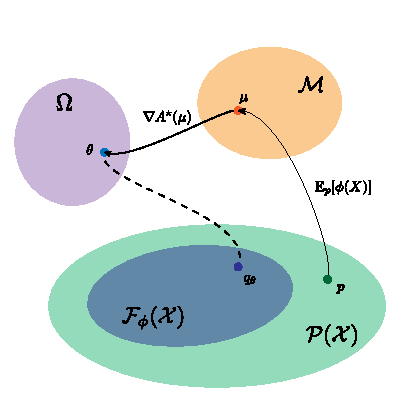
\includegraphics[width=.5\textwidth]{figures/expf/mapping2}
%\caption{blah}
%\end{figure}
This is supported by the fact that this distribution actually minimises the divergence $\KL{p,q_{\theta'}}$. Indeed, observe that
%
\eqa{
	\KL{p,q_{\theta'}} &=& \E_{p}[\log p] - \scal{\theta', \mu} + A(\theta'), \label{kldivadf}
}
%
which is a strictly convex function in $\theta'$. By definition, a parameter $\theta=\nabla A^{\star}(\mu)$ is such that $\nabla A(\theta)=\mu$ and therefore verifies the first order condition. This shows that $q_{\theta}$ minimises the divergence \eqref{kldivadf}. It is useful at this point to define a projection operator $\mathbf P_{\phi}:\mathcal P(\mathcal X) \to \mathrm{cl}(\Omega)$\, with
%
\eqa{	
	\theta \,\,=\,\, \mathbf P_{\phi}[p] &\Longleftrightarrow& \theta \,\,=\,\, \nabla A^{\star}(\E_{p}[\phi(X)]).
}
%
Assuming $\mathbf P_{\phi}[p] \in \Omega$, $q_{\theta}$ is a proper distribution in $\mathcal F_{\phi}(\mathcal X)$ that minimises the KL \eqref{kldivadf} and equivalently verifies the \emph{global moment matching condition} (GMMC) 
%
\eqa{
	(\text{GMMC})\qquad \E_{q_{\theta}}[\phi(X)]&=&\E_{p}[\phi(X)].
\label{eq:GMMC}}
%
It will also be convenient to use the following abuse of notation: for an unnormalised distribution $p_{u}$ with some normalisation constant $Z_{p_{u}}\inv$ we will write $\mathbf P_{\phi}[p_{u}]$ to implicitly mean $\mathbf P_{\phi}[Z_{p_{u}}\inv p_{u}]$.\check{april 24}

The application of this projection operator implicitly requires the ability to perform two computations. First, it requires the ability to compute the expected value $\mu=\E_{p}[\phi(X)]$ which is typically intractable since we are in a context where we are trying to approximate $p$ for that very purpose. Then, provided we can compute $\mu$, we need to be able to apply the inverse mapping $\nabla A^{\star}(\mu)$. We will introduce below contexts in which the first requirement can be approximately met. The second requirement effectively means that we are constrained to exponential families for which computing the inverse mapping $\nabla A^{\star}$ can be done explicitly or is cheap to approximate. For continuous state spaces, it is overwhelmingly the Gaussian distribution that is considered in the literature with either a diagonal or a full covariance matrix.\add{probably add a section here on how to compute forward backward operator, maybe put this in appendix. Also cite lots of stuff that uses the Gaussian, if you find anything that doesn't...}\check{april24} 
%
% ----------------------------------------
\subsubsection*{Online Bayesian Learning and Assumed Density Filtering}
%
Let us consider the context of online Bayesian learning where one is interested in the evolution of a posterior distribution $p(x\st y_{1:t})$ given observed \iid\add{notations iid} data points $y_{1:t}$ up to current time $t$ and a new \iid data point $y_{t+1}$. The new posterior is given directly by Bayes rule with $p(x\st y_{1:t+1})\propto p(y_{t+1}\st x) p(x\st y_{1:t})$. In \citet{opper98}, the author considers that the exact posteriors are intractable but suggests constructing a sequence of approximations in the exponential family $\mathcal F_{\phi}(\mathcal X)$. Using the notations from the previous point, the algorithm corresponds to a sequence of iteration of the form
\eqa{	\theta_{t+1} &=& \mathbf P_{\phi}[p(y_{t+1}\st \cdot)q_{\theta_{t}}],	\label{adfonline}}
where, at the first step, $q_{\theta_{0}}$ is replaced by the prior $\pi_{0}$. In words, the posterior up to time $t$ is approximated by the exponential family distribution $q_{\theta_{t}}$ which then serves as prior to form an approximate posterior $p(y_{t+1}\st x)q_{\theta_{t}}(x)$. Given that this approximate posterior is not necessarily in the exponential family, it needs to be projected as per \eqref{adfonline}.\check{april27} At time $t+1$, the distribution $q_{\theta_{t+1}}$ can be now interpreted as an approximation of the posterior distribution given all the data up to that time or 
%
\eqa{	q_{\theta_{t+1}}(x) \esp\approx\esp p(x) &\propto& \pi_{0}(x)\prod_{s=1}^{t+1}p(y_{s}\st x).
}
%
We can therefore reinterpret the algorithm more generally as targeting a distribution $p$ that factorises in a fixed number (say $K$) of factors: $p(x)\propto \pi_{0}(x)\prod_{i=1}^{K}t_{i}(x)$.\add{notations: make sure it's clear that $\pi_{0}$ is always the prior} This is the Assumed Density Filtering algorithm. Note that in this case there is no ``natural ordering'' as in the online learning case and the algorithm can be done with any permutation of the factors.\check{april27}

\begin{algorithm}[!h]\small
	\caption{\label{alg:adf}\dblue{\emph{\small Assumed Density Filtering}}}
	\begin{algorithmic}[1]
	\State Let $\theta_{1}=\mathbf P_{\phi}[\pi_{0}t_{1}]$
	\For{$i=2:K$}
		\State $\theta_{i}\leftarrow\mathbf P_{\phi}[q_{\theta_{i-1}}t_{i}]$ \Comment{parameter of the new approximation}
%		\State $\omega_{i} \leftarrow \theta_{i}-\theta_{i-1}$\Comment{parameter of the local approximation}
	\EndFor\\
	\Return{$\theta_{K}$}
	\end{algorithmic}
\end{algorithm} 

Let $\omega_{i}=(\theta_{i}-\theta_{i-1})$ denote the difference between subsequent parameters (with $\omega_{1}=\theta_{1}$). Correspondingly $\theta_{K}=\sum_{i=1}^{K}\omega_{i}$, and letting $\tilde t_{i}(x):=\exp\scal{\omega_{i},\phi(x)}$, which can be interpreted as an approximation to the factor $t_{i}$, we can write 
%
\eqa{
	q_{\theta_{K}}(x) &\propto& \pi_{0}(x)\prod_{i=1}^{K}\tilde t_{i}(x).\label{eq:approxadf}
}
% 
The main issue with using ADF on an MRF is that the order in which the graph is read or equivalently the order in which the factors $t_{i}$ are considered will affect the final approximation $q_{\theta_{K}}$. A natural extension is then to perform ADF multiple times considering random orderings of the factors and to adjust the approximation accordingly. This is the Expectation Propagation algorithm.\check{april27}
%
% --------------------------------------
\subsubsection*{Expectation Propagation}
%
In the Expectation Propagation algorithm \citep{minka01, minka01b, seeger07, gelman14}, we consider that we have an initial approximation $q_{\theta}\in\mathcal F_{\phi}(\mathcal X)$ that we can write as in \eqref{eq:approxadf} (typically obtained with a pass of ADF) and we seek to iteratively improve its parameter $\theta$. At each step, a factor $t_{i}$ is considered and, by contrast to ADF, we now consider the projection $\theta_{i}=\mathbf P_{\phi}[q_{\theta}t_{i}/\tilde t_{i}]$. The difference with ADF is therefore the removal of the previous factor approximation $\tilde t_{i}$ from the current approximation $q_{\theta}$ before the projection. ADF can also be reinterpreted as EP where, initially, all the factor approximations are set to $\tilde t_{i}\equiv 1$.\check{april27}

\begin{algorithm}[!h]\small
	\caption{\label{alg:ep}\dblue{\emph{\small Expectation Propagation}}}
	\begin{algorithmic}[1]
	\State Initialise $\theta,\omega_{1},\dots,\omega_{K}$ such that $\theta=\sum_{i=1}^{K}\omega_{i} \in \Omega$ (e.g. via ADF)
	\For{$k=1:N_{\text{EP}}$}
		\State Let $\sigma$ be a random permutation of $(1,\dots,K)$
		\For{$i=1:K$}
    		\State $\theta \leftarrow \mathbf P_{\phi}[q_{\theta^{\text{old}}}t_{\sigma(i)}/\tilde t_{\sigma(i)}]$\Comment{\emph{parameter of the new global approximation}}
    		\State $\omega_{\sigma(i)} \leftarrow \omega_{\sigma(i)} + \theta-\theta^{\text{old}}$\Comment{\emph{parameter of the new factor approximation $\tilde t_{\sigma(i)}$}}
			\State $\theta^{\text{old}} \leftarrow \theta$
		\EndFor
	\EndFor\\	
	\Return{$\theta$}
	\end{algorithmic}
\end{algorithm} 

In Expectation Propagation, we denote by $q_{-i}\propto q_{\theta}/\tilde t_{i}$ a \emph{cavity distribution} and by $q_{i}\propto q_{-i}t_{i}$ a \emph{tilted distribution} \cite{gelman14}. If the EP algorithm converges, then the global parameter $\theta$ is necessarily such that all the \emph{local moment matching conditions} (LMMC) are met:
%
\eqa{
	(\text{LMMC})\qquad	\E_{q_{i}}[\phi(X)]=\E_{q_{\theta}}[\phi(X)], \quad i=1,\dots,K.\label{eq:LMMC}
} 
%
These conditions can be interpreted as a relaxation of the GMMC \eqref{eq:GMMC} and the EP algorithm can be interpreted as a fixed point algorithm targeting the LMMC.\add{depending on how much you discuss in SNEP, link here to that part and say will discuss in more details.}\add{maybe add ``expectation consistent inference'' the stuff by Heskes etc}


%%%%%%%%%%%%%%%%%%%%%%%%%%%%
\section{Belief Propagation}

\todofr{
    \begin{itemize}\itsep0
    	\item BP on a tree
		\item LBP when iterating
		\item why is it / is it not a good idea (energy min and MERL stuff)
	\end{itemize}
}

% ==================
\section{Discussion}
\todofr{
(see where stuff belongs, either here or in previous points)
\begin{itemize}\itsep0
	\item more literature quotations probably especially indicating the different pieces of work for different applications (?)
	\item can do expoF but in practice people do Gaussian, why
	\item EP energy and showing that it's not really justified, maybe drawing where you show that VB arrives to a point (convergence guarantees, no guarantee of quality), EP goes to a point (no convergence guarantee, no guarantee of quality) and so that we're a bit in the dark. See whether Gelman discusses VB vs EP...
	\item poor recovery of variance, why
	\item link EP, BP, show BP can be interpreted as EP
	\item other, non-KL recovery, make link with choice of loss function in general, discuss that (maybe)
	\item power EP from EP (maybe in SNEP or in EPBP when discussing extensions see how can include story)
	\item comparison VI and MAP (choice of loss function, popularity etc.)
\end{itemize}
}\fi

\chapter[EPBP]{Expectation Propagation for\\ Particle Belief Propagation}

\ifpbp% !TEX root = ../thesis.tex

In this chapter, we look at ways to implement the loopy belief propagation (LBP) algorithm on an arbitrary MRF with continuous state-spaces. We concentrate in particular on the representation of the messages and the computation of message updates in the LBP algorithm. 

In this chapter, we consider the \emph{nonparametric belief propagation} (NBP) algorithm of \citet{sudderth03} and the \emph{particle belief propagation} algorithm of \citet{ihler09}. We then discuss our \emph{expectation particle belief propagation} (EPBP) algorithm \citep{lienart15} and discuss how it improves upon both. \check{jul19}

% !!!!!!!!!!!!!!!!!!!!!!!!!!!!!!!!!!!!!!!!!!!!!!!!!!!!!!!!!!!!!!!!!!!!!!!!!!!!!!!!!!!!!!!!!!!!!!!!!!
\section{Loopy Belief Propagation on Continuous State-Spaces}
At point \ref{point:LBP}, we had shown that, at iteration $n$ of the LBP algorithm, the messages are obtained by computing the following integral:
\eqa{
	m^{n}_{ts}(x_{s}) &=& \int \psi_{st}(x_{s},x_{t})M^{n}_{t s}(x_{t})\dx_{t}\label{eq:mess-update-2}
}
where the pre-messages are given by 
\eqa{
	M_{st}^{n}(x_{s}) &=& \psi_{s}(x_{s}) \prod_{r\in\partial s\backslash t} m^{n-1}_{rs}(x_{s}).
}
Ultimately, we are interested in computing the beliefs obtained by multiplying message and pre-message: $B_{s}^{n}(x_{s}) = m^{n}_{ts}(x_{s})M^{n}_{st}(x_{s})$. There are a few main computational problems to tackle when attempting to run this algorithm in a continuous setting. First, the messages need to be represented in a tractable fashion. Second, the message updates need to be computable and the results easily expressible in the chosen representation system. Lastly, we need to be able to easily compute expected values with respect to the resulting estimators for the beliefs. We discuss below two existing methods attempting to tackle those issues.
%%%%%%%%%%%%%%%%%%%%%%%
\subsection{Nonparametric belief propagation}

In \citet{sudderth03}, the authors suggest representing the messages in the LBP iterations as mixtures of Gaussians:
\eqa{	
	\widehat m^{\text{NBP}}_{ts}(x_{s}) &:=& \sum_{i=1}^{M} w_{s}^{i}\,\mathcal N(x_{s};\mu^{i}_{s},\Lambda_{s}). \label{eq:nbp-representation}
}
They call their algorithm \emph{nonparametric belief propagation} (NBP). In order to make computations more efficient, the authors restrict the covariance matrices to be diagonal.\add{mention this in general complaint for VI}
As indicated in the paper, the representation \eqref{eq:nbp-representation} makes sense only when the messages are finitely integrable. To guarantee this, the authors require that all potentials satisfy the following constraints:
\eqa{	
	\sup_{x_{t}} \int \psi_{st}(x_{s},x_{t})\dx_{t} &<&\infty, \quad \text{and}\quad \int \psi_{s}(x_{s})\dx_{s} \esp<\esp \infty,\label{conditions NBP}
}
where the integrals are taken over the range of admissible values for the relevant variable. Provided these assumptions hold, the message updates are well defined and can be explicitly (and efficiently) computed. Computing the beliefs however, requires considering the product of mixtures of $M$ terms leading to a complex representation and an explosion in computational cost. In order to alleviate this, the authors suggest an importance sampling approach targeting the beliefs and fitting mixtures of Gaussians to the resulting weighted particles. 
The computation of the message updates \eqref{eq:mess-update-2} is thereby always done over a constant number of terms.\check{jul19}

\subsubsection*{Main issues}

A key weakness of the NBP algorithm is that the conditions \eqref{conditions NBP} do not hold in a number of important cases (the authors aknowledge this in a footnote of their paper). 
First, the node potentials $\psi_{u}$ are usually proportional to likelihoods of the form $p(y_{u}\st x_{u})$ which need not be integrable in $x_{u}$. In fact, for most non-Gaussian potential, this is the case. Then, there exist applications for which the first integrability condition on edge potentials does not hold. In imaging applications for example, the edge potential can encode a measure of similarity between pixels which need not verify the first integrability condition as in \citet{nikolova00}. Finally, by definition of NBP as an approximated representation with a fixed number of Gaussians, it does lead to consistent estimators of the LBP messages.\check{jul24, jul21, jul19}



%%%%%%%%%%%%%%%%%%%%
\subsection{\label{point:PBP}Particle belief propagation}

In \citet{ihler09}, the authors suggest a way to overcome the shortcomings of NBP by considering importance sampling to tackle the update of the LBP messages instead of working with mixtures of Gaussians. For a chosen proposal distribution $q_{u}$ on node $u$ and a draw of $N$ particles $X_{u}^{(i)}\simiid q_{u}$, the messages are represented via an importance sampling estimator of the corresponding integral:
\eqa{		
	&\widehat m_{st}^{\text{PBP}}(x_{t}) 
		:= \sum_{i=1}^{N}w^{(i)}_{st}\psi_{st}(X^{(i)}_{s},x_{t}), \quad\text{where}&	\label{eq:rep-PBP}\\[.4cm]
	&w^{(i)}_{st} 
		\esp\!\propto\esp\! \displaystyle{\widehat M^{\text{PBP}}_{st}(X_{s}^{(i)})\over q_{s}(X_{s}^{(i)})}, \quad\text{and}\quad
	\widehat M^{\text{PBP}}_{st}(x_{s}) \esp\!=\esp\! \psi_{s}(x_{s}) \prod_{r\in\partial s\backslash t} \widehat m^{\text{PBP}}_{rs}(x_{s}).&\nn
}

They call their algorithm \emph{particle belief propagation} (PBP).
This algorithm has the advantage that it does not explicitly require the integrability conditions \eqref{conditions NBP} to hold. 
In terms of choosing proposals, the authors suggest two potential choices: sampling from the local potential $\psi_{s}$, or sampling from the current belief estimate on the node. 
%For the latter, the authors suggest running a short MCMC simulation. \add{explain how they build representation of beliefs}

\subsubsection{Main issue}

The weak point of the PBP algorithm is the choice of proposal distributions.  A poor choice will lead to poor estimators of the messages which, over a few iterations of the LBP algorithm, can lead to poor representations of the beliefs.

The first suggestion by the authors to sample from the local potential is only valid if $\psi_{s}$ is integrable which, as we have mentioned earlier, is not the case in general. The second suggestion implies sampling from a distribution of the form
%
\eqa{		
	\widehat B_{s}^{\text{PBP}}(x_{s}) 
		&\propto& \psi_{s}(x_{s}) \prod_{r\in\partial s} \widehat m^{\text{PBP}}_{rs}(x_{s})	\label{eq:PBP proposal}
}
%
which is a product of mixtures of $N$ components. As in nonparametric BP, naive sampling of the proposal has complexity $\mathcal O {(N^{|\partial {s}|})}$ and is thus, in general, too expensive to consider.

Alternatively the author suggest running a short MCMC simulation targeting it which reduces the complexity to order $\mathcal O {(|\partial {s}|N^{2})}$. Indeed, each MCMC iteration requires evaluating $\widehat B_{s}^{\text{PBP}}$ point-wise which has complexity $\mathcal O {(|\partial{s}|N)}$, and we need at least $\mathcal{O}(N)$ iterations of the MCMC simulation to produce the samples. Note that it is unclear how many more iterations are necessary to get $N$ \emph{good} samples. Running a short MCMC chain (to reduce computational cost) will therefore almost certainly lead to biased samples. In the code the authors shared with us, they run $N$ parallel random walk Metropolis-Hastings chains \citep[chapter 6]{robert04} for a fixed number of steps. This choice may have been motivated by a desire to control the complexity of the algorithm more accurately but it is at the expense of the quality of the samples obtained.

%%%%%%%%%%%%%%%%%%%%%%%%
\section{Expectation Particle Belief Propagation}
As for the PBP algorithm, we consider importance sampling to build particle representations of the messages. In our method, however, we consider a \emph{sequence} of proposal distributions at each node from which one can cheaply sample particles at a given iteration of the LBP algorithm. 

The novelty of the approach is to propose a principled and automated way of designing a sequence of proposals in a tractable exponential family using the expectation propagation (EP) algorithm. The resulting method, which we call \emph{Expectation Particle Belief Propagation} (EPBP), does not suffer from the restrictive integrability conditions of the NBP algorithm and sampling is done exactly unlike the PBP algorithm which implies that we obtain consistent estimators of the LBP messages.

Further, the development of our method also formally shows that considering proposals close to the beliefs, as suggested by \cite{ihler09}, is a good idea.  Our core observation is that since sampling from a proposal of the form \eqref{eq:PBP proposal} using MCMC simulation is very expensive, we should consider using a more tractable proposal distribution instead. However it is important that the proposal distribution is constructed adaptively, taking into account evidence collected through the message passing itself. We propose to achieve this by using proposal distributions lying in a tractable exponential family, and adapted using EP.

%%%%%%%%%%%%%%%%
\subsection{Proposal selection for PBP}
In this point we discuss the ideal choice of proposal distributions when considering the PBP algorithm. We consider two connected nodes $s$ and $t$ at a a given iteration and assume we have already constructed particle based representations of all incoming messages into both $s$ and $t$ apart from the messages from $s$ to $t$ and from $t$ to $s$. 
We therefore have both pre-messages $\widehat M_{st}$ and $\widehat M_{ts}$ of the form:
%
\eqa{
	\widehat M_{st}(x_{s}) &\propto& \psi_{s}(x_{s}) \prod_{r\in \partial s \backslash t} \widehat m_{rs}(x_{s}).
}
%
This is illustrated at figure \ref{representation-edge-pbp}. 

\begin{figure}[!h]
\center
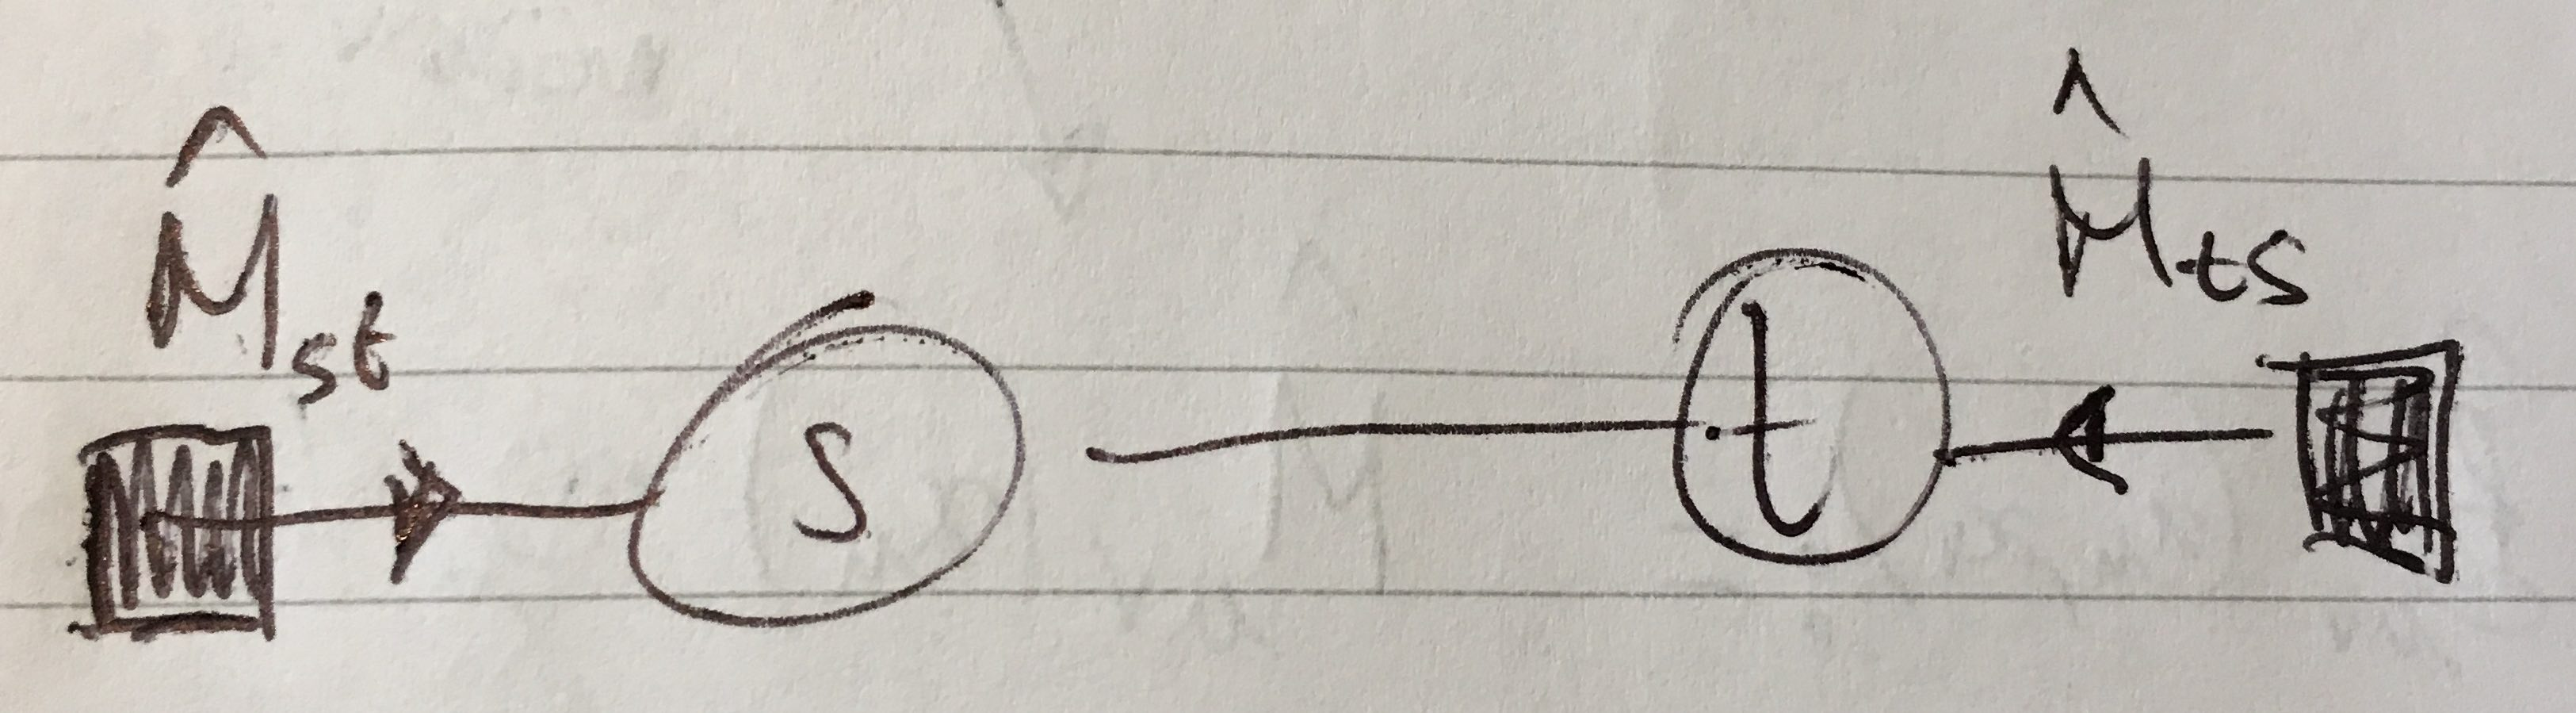
\includegraphics[width=.7\textwidth]{figures/draft/schema_pbpsel}
\caption{\label{representation-edge-pbp}}
\end{figure}

We would like to define $q_{s}$ and $q_{t}$ in a joint manner in such a way that all objects remain consistent with the LBP iterations. For that reason, we consider the joint belief $ B_{st}$ on $s$ and $t$ given the approximation to the pre-messages:
%
\eqa{	
	 B_{st}(x_{s},x_{t}) &\propto& \widehat M_{st}(x_{s}) \psi_{st}(x_{s},x_{t})\widehat M_{ts}(x_{t}).
}
%
The marginals of the joint belief are of the form
%
\eqa{
	B_{st}(x_{s}) &\propto& \widehat M_{ts}(x_{s}) \int \psi_{st}(x_{s},x_{t}) \widehat M_{ts}(x_{t})\dx_{t}\nn\\
	&\propto & \widehat M_{st}(x_{s}) m_{ts}(x_{s}),
}
%
where $m_{ts}$ is the exact (but intractable) LBP message given the pre-message approximation $\widehat M_{ts}$.
Following our point about defining $q_{s}$ and $q_{t}$ in a joint manner, let us consider $q_{s}q_{t}$ as a proposal for the joint belief $ B_{st}$.
We can then define an empirical distribution for it:
%
\eqa{
	\widehat{B}_{st}(x_{s},x_{t}) &\propto& \sum_{i,j=1}^{N} {\widehat M_{st}(X_{s}^{(i)})\psi_{st}(X_{s}^{(i)},X_{t}^{(j)})\widehat M_{ts}(X_{t}^{(j)}) \over q_{s}(X_{s}^{(i)})q_{t}(X_{t}^{(j)})} \delta_{(X_{s}^{(i)},X_{t}^{(j)})}(x_{s},x_{t}). \label{eq:pbp-particle-joint-belief}
}
%
Marginalising this approximation over $x_{t}$ leads to
%
\eqa{
	\widehat{B}_{st}(x_{s}) &\propto& \sum_{i=1}^{N} {\widehat M_{st}(X_{s}^{(i)}) \widehat { m}_{ts}(X_{s}^{(i)}) \over q_{s}(X_{s}^{(i)})} \delta_{X_{s}^{(i)}}(x_{s}). \label{eq:pbb-particle-joint-belief-marg}
}
%
where $\widehat{m}_{ts}$ is the importance sampling estimator for $ m_{ts}$ using $q_{t}$ as proposal. Of course, marginalising \eqref{eq:pbp-particle-joint-belief} over $x_{s}$ leads to an expression analogous to \eqref{eq:pbb-particle-joint-belief-marg}. Focusing on node $s$, the expression \eqref{eq:pbb-particle-joint-belief-marg} indicate that the proposals should be given by
%
\eqa{
	q_{s}(x_{s}) &\propto& \widehat{M}_{st}(x_{s}) \widehat{m}_{ts}(x_{s}) \esp = \esp \psi_{s}(x_{s}) \prod_{r\in\partial s} \widehat{m}_{rs}(x_{s})
	}
where all $\widehat m_{rs}$ are importance sampling estimators built using the corresponding most recent $q_{r}$ as a proposal. Further, this shows that the proposals on nodes should correspond to the most recent approximation of the belief at that node which aligns with the suggestion in \citet{ihler09}.

%%%%%%%%%%%%%%%%
\subsection{The EPBP algorithm}
As we showed in point \ref{point:PBP}, it is computationally expensive to use the particle approximated node belief as the proposal distribution. 
Our idea is therefore consider an approximation $q_{s}$ drawn from a tractable exponential family $\mathcal F_{\phi}$ with a structure matching that of the belief:
%
\eqa{ 
	q_s(x_s) &\propto& \eta_{\circ s}(x_s) \prod_{r\in\partial s} \eta_{rs}(x_s).
}
%
In the experiments we used a Gaussian family but the algorithm is -- in theory  -- not limited to this choice.
Using the framework of expectation propagation (EP) that we discussed in point \ref{point:EP}, we can iteratively find good proxies to the node belief in the exponential family.

For each $r\in\partial s$, we update the $\eta_{rs}$ following the EP framework. We start by forming the \emph{cavity} $q^{\backslash r}_{s}=q_{s}/\eta_{rs}$ and the corresponding \emph{tilted distribution} proportional to $\widehat m_{rs} q_{s}^{\backslash r}$.  The updated distribution is then the projection of the tilted distribution onto the exponential family manifold:
\eqa{ q_{s} &\leftarrow& \mathbf P_{\phi}[\widehat m_{rs}q_{s}^{\backslash r}],}	
where $\mathbf P_{\phi}$ is the projection operator defined at \ref{eq:def-proj-operator-ep}. Consequently, the factor $\eta_{rs}$ is updated: $\eta_{rs} \leftarrow  q_{s}/ q_{s}^{\backslash r}$. Note that other projection mechanisms than projecting with respect to the Kullback-Leibler divergence can be considered as well. 

In the algorithm as we have described it so far, the EP steps for each incoming message into $s$ and for the node potential are performed first in order to fit the proposal to the current estimated belief at $s$. Then, this estimated belief is used to draw $N$ particles which can be used to form the particle approximated messages from $s$ to each of its neighbours. 
Alternatively, once each particle approximated message $\widehat{m}_{st}(x_t)$ is formed, we can update their exponential family projections $\eta_{st}(x_t)$ immediately. This is the scheme described in algorithm \ref{alg:epbp-node-update}.

\begin{algorithm}[!h]\small
	\caption{\label{alg:epbp-node-update}\idblue{\small Node update in the EPBP algorithm}}
	\begin{spacing}{1.2}
	\begin{algorithmic}[1]
		\State sample $\{X^{(i)}_{s}\}_{i=1}^{N}\simiid q_{s}$	
		\State evaluate the approximate representation of the belief: $$\widehat B_{s}(X_{s}^{(i)}) = \psi_{s}(X_{s}^{(i)})\prod_{r\in\partial {s}}\widehat m_{rs}(X_{s}^{(i)})$$% $q_{u}(x_{u}^{(i)})$
		\For{$v\in \partial {u}$}
			\State evaluate the approximate representation of the pre-message: $$\widehat M_{st}(X_{s}^{(i)}) :=\widehat B_{s}(X_{s}^{(i)})/\widehat m_{ts}(X_{s}^{(i)})$$
			\State compute the corresponding normalised weights $$ w_{st}^{(i)}\propto \widehat M_{st}(X_{s}^{(i)})/q_{s}(X_{s}^{(i)})$$
			\State update the estimator of the outgoing message: $$\widehat m_{st}(x_{t})=\sum_{i=1}^{N}w^{(i)}_{st}\psi_{st}(X_{s}^{(i)},x_{v})$$
			\State update $\eta_{\circ t}$ to match the update $q_{t} \leftarrow \mathbf P_{\phi}[\psi_{t}q_{t}/\eta_{\circ t}]$ 
			\State update $\eta_{st}$ to match the update $q_{t}\leftarrow \mathbf P_{\phi}[\widehat m_{st}q_{t}/\eta_{st}]$% and update $\eta_{uv}$ correspondingly %compute the cavity distribution $q^{\backslash u}_{v}\propto q_{v}/\eta_{uv}$, get $\eta^{+}_{uv}$ in the exponential family such that $\eta^{+}_{uv}q_{v}^{\backslash u}$ approximates $\widehat m_{uv}q_{v}^{\backslash u}$, update $q_{v}\propto \eta_{uv}^{+}$ and let $\eta_{uv}\leftarrow \eta_{uv}^{+}$
		\EndFor
	\end{algorithmic}
	\end{spacing}
\end{algorithm}

Note that, in the EP step, if the projection leads to an invalid distribution (e.g., in the Gaussian case, if it leads to an element with negative variance), we simply revert the approximation to its previous value as in \citet{minka01}. \add{this should be discussed in EP intro}

%%%%%%%%%%%%%%%%%%
\subsection{Projection mechanisms}

In the description above, we used the projection $\mathbf P_{\phi}$ from \ref{eq:def-proj-operator-ep}. 
Computing this projection requires computing the moments of the tilted distribution. 
Since this is usually intractable, we have to resort to numerical quadrature. 
In our scenario the moment computation can be performed crudely on a small number of integration points since it only concerns the updating of the importance sampling proposal. 
Since the dimensionality of the tilted distribution in the EPBP algorithm is typically low, a simple deterministic quadrature rule can be used \citep{davis75}. \\

The key desired element for the projection is that the resulting updated proposal distribution captures the support of the current estimator of the belief on the node. Since this is a rather general requirement, the KL-projection $\mathbf P_{\phi}$ does not necessarily lead to the best proposals and in fact may suffer from the fact that we have to compute the projection from the mean-parameter space to the natural parameter space $\nabla A^{\star}$ associated with the exponential family of interest which may be numerically unstable.  
This can be mitigated by damping as described at point \dred{XXXXX}\add{link} but alternative projection schemes can be tried as well.
In our experiments for example, we tried considering the $q_{s}\in\mathcal F_{\phi}$ obtained by doing a maximum likelihood estimation of the natural parameters based on a small number of evaluation points of the tilted distribution. This proved to work well in practice.

%%%%%%%%%%%%%%%%%%%%%%
\subsection{\label{sec:EPBP-compcompl}Computational complexity}
The steps that dominate in terms of computational complexity is the evaluation of the approximate representation of the pre-message.
Since the estimator for the belief is a product of $|\partial s|$ mixtures of $N$ components, evaluating at $N$ sampling points is $\mathcal O(|\partial s|N^{2})$. 
Further, the evaluation of the pre-message requires evaluating the message $\widehat m_{ts}$ at $N$ sampling points. Since $\widehat m_{ts}$ is a mixture of $N$ components, this also has quadratic complexity. The dominating complexity of the EPBP algorithm is therefore $\mathcal O(KEN^{2})$ where $K$ is the number of passes done over the graph, and $E$ is the number of edges in the graph.

This inherent quadratic complexity can be reduced. Indeed, instead of we can follow a method presented in \cite{briers05} to sample from a product of mixtures where one draws, for each mixture $\widehat m_{st}$, a set of $M$ indices $\{i^{\star}_{\ell}\}_{\ell=1}^{M}$ from a multinomial with weights $\{w^{i}_{st}\}_{i=1}^{N}$ and samples from a mixture of the corresponding $M$ terms $\psi^{i^{\star}_{\ell}}_{st}$. 
This reduces the cost of the evaluation of the belief to $\mathcal O(|\partial {s}|MN)$ where $M$ is taken to be sub-quadratic in $N$. 
We show in the next section that this version of the algorithm still compares favourably to the quadratic implementation with $M = \mathcal O(\log N)$. 



%%%%%%%%%%%%%%%%%
%\subsection{EPBP for smoothing} % requires backward sampling.

%%%%%%%%%%%
\section{Experiments}

We investigate the performance of our method on MRFs for two simple graphs. This allows us to compare the performance of EPBP to the performance of PBP in depth. We also illustrate the behaviour of the sub-quadratic version of EPBP. Finally we show that EPBP provides good results in a simple denoising application, an example on which the PBP implementation of \citet{ihler09} would struggle to give results in a reasonable time due to its dimensionality.

\subsection{Grid and tree experiments}
We start by comparing EPBP to PBP as implemented by \citet{ihler09} on a $3\times 3$ grid (see \fig{fig:grids} (left)) with random variables taking values on $\mathbb R$. The node and edge potentials are selected such that the marginals are multimodal, non-Gaussian and skewed with
\eqa{	
	\left\{
		\begin{array}{lcl}
			\psi_{u}(x_{u}) &=& \alpha_{1}\mathcal N(x_{u}-y_{u}; \mu_{1},\sigma_{1})+\alpha_{2}\mathcal G(x_{u}-y_{u};\mu_{2},\beta)\\
			\psi_{uv}(x_{u},x_{v}) &=& \mathcal L(x_{u}-x_{v};\mu_{3},\sigma_{3})
		\end{array}
	\right.,
}
%-2, 1, 2, 1.3, 0, 2
where $y_{u}$ denotes the observation at node $u$, $\mathcal N(x;\mu,\sigma)\propto \exp(-x^{2}/2\sigma^{2})$ (density of a Normal distribution), $\mathcal G(x;\mu,\beta)\propto \exp(-[(x-\mu)/\beta+\exp(-(x-\mu)/\beta)])$ (density of a Gumbel distribution) and $\mathcal L(x;\mu,\beta)\propto \exp(-|x-\mu|/\beta)$ (density of a Laplace distribution). The parameters were set in an arbitrary fashion to:
$$ \alpha_{1}=0.6,\,\, \alpha_{2}=0.4,\,\, \mu_{1}=-2,\,\,\mu_{2}=2,\,\,\mu_{3}=0, \,\,\sigma_{1}=1, \,\,\sigma_{2}=2, \,\,\beta=1.3. $$
We compare the two methods after 20 LBP iterations.\footnote{The scheduling used alternates between the classical orderings: top-down-left-right, left-right-top-down, down-up-right-left and right-left-down-up. One ``LBP iteration'' implies that all nodes have been updated once.} 
We then repeated the experiments on a tree with 8 nodes (\fig{fig:grids} (right)) where we know that, at convergence, the beliefs computed using BP are proportional to the true marginals. Again, the node and edge potentials are picked such that the marginals are multimodal with this time
\eqa{	
	\left\{
		\begin{array}{lcl}
			\psi_{u}(x_{u}) &=& \alpha_{1}\mathcal N(x_{u}-y_{u}; \mu_{1},\sigma_{1})+\alpha_{2}\mathcal N(x_{u}-y_{u};1\mu_{2},\sigma_{2})\\
			\psi_{uv}(x_{u},x_{v}) &=& \mathcal L(x_{u}-x_{v};\mu_{3},\sigma_{3})
		\end{array}
	\right.,
}
with the parameters also set in an arbitrary fashion to:
$$\alpha_{1}=0.3,\,\,\alpha_{2}=0.7,\,\,\mu_{1}=-2,\,\,\mu_{2}=1,\,\,\mu_{3}=0,\,\,\sigma_{1}=1,\,\,\sigma_{2}=0.5,\,\,\sigma_{3}=1.$$
On this second example, we also considered ``pure EP'' with Gaussians to compare with EPBP and PBP. 


\begin{figure}[!h]
\center
%\vspace*{-.3cm}
	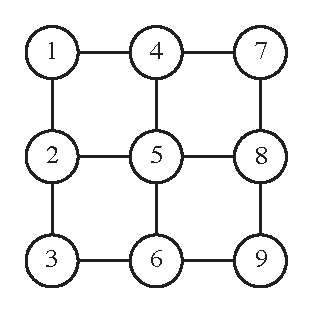
\includegraphics[width=.3\textwidth]{figures/epbp/grid33}
	\hspace*{1cm}
	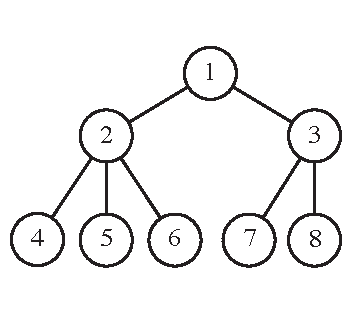
\includegraphics[width=.3\textwidth]{figures/epbp/tree8}
%\vspace*{-.5cm}
	\caption{\label{fig:grids}Illustration of the grid (left) and tree (right) graphs used in the experiments.}
\end{figure}

PBP as presented in \citet{ihler09} is implemented using the same parameters than those in an implementation code provided by the authors: the proposal on each node is the last estimated belief and sampled with a 20-step MCMC chain, the Metropolis Hastings proposal is a normal distribution. For EPBP, the approximation of the messages are Gaussians. The ground truth is approximated by running LBP on a deterministic equally spaced mesh with 200 points. All simulations were run with Julia on a Mac with 2.5 GHz Intel Core i5 processor, our code is available online.\footnote{\url{https://github.com/tlienart/EPBP}.} All the experiments were run multiple times as shown on the figures to account for the inherent stochasticity of the methods. The mean trends are also drawn.
%%%%%%%%%%%%%%%%%%%%%%%%%%%
%\subsubsection{Results of the grid and tree experiments}

The \fig{figCompGrid} compares the performances of both methods. The error is computed as the mean $L^{1}$ error over all nodes between the estimated beliefs and the ground truth. One can observe that not only does PBP perform worse than EPBP but also that the error plateaus with increasing number of samples. This is because the sampling within PBP is done approximately and hence the consistency of the estimators is lost. Note that for EPBP, one observes the expected $1/\sqrt{N}$ convergence of particle methods discussed in \citet{ihler09}.

\begin{figure}[!h]
\center
%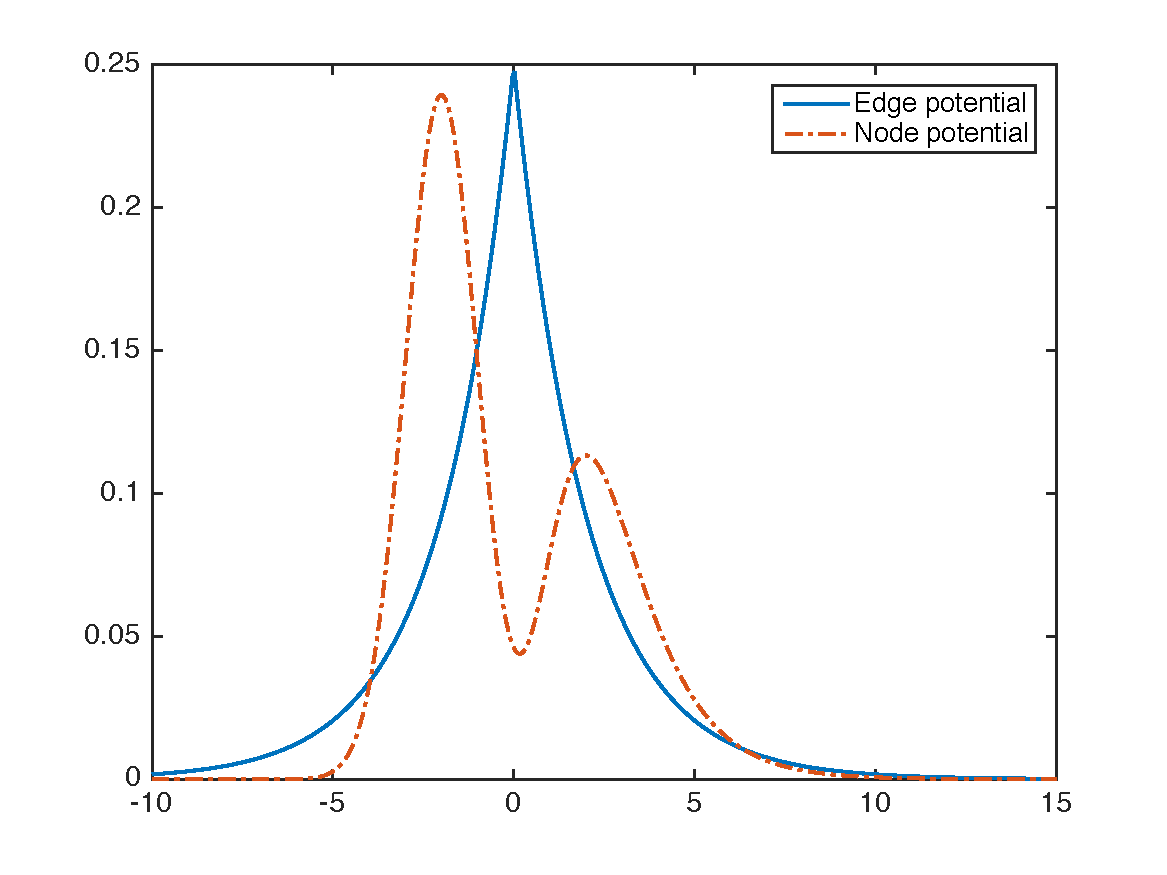
\includegraphics[scale=.25]{figs/node_edge_pot}
%\hspace*{-.6cm}
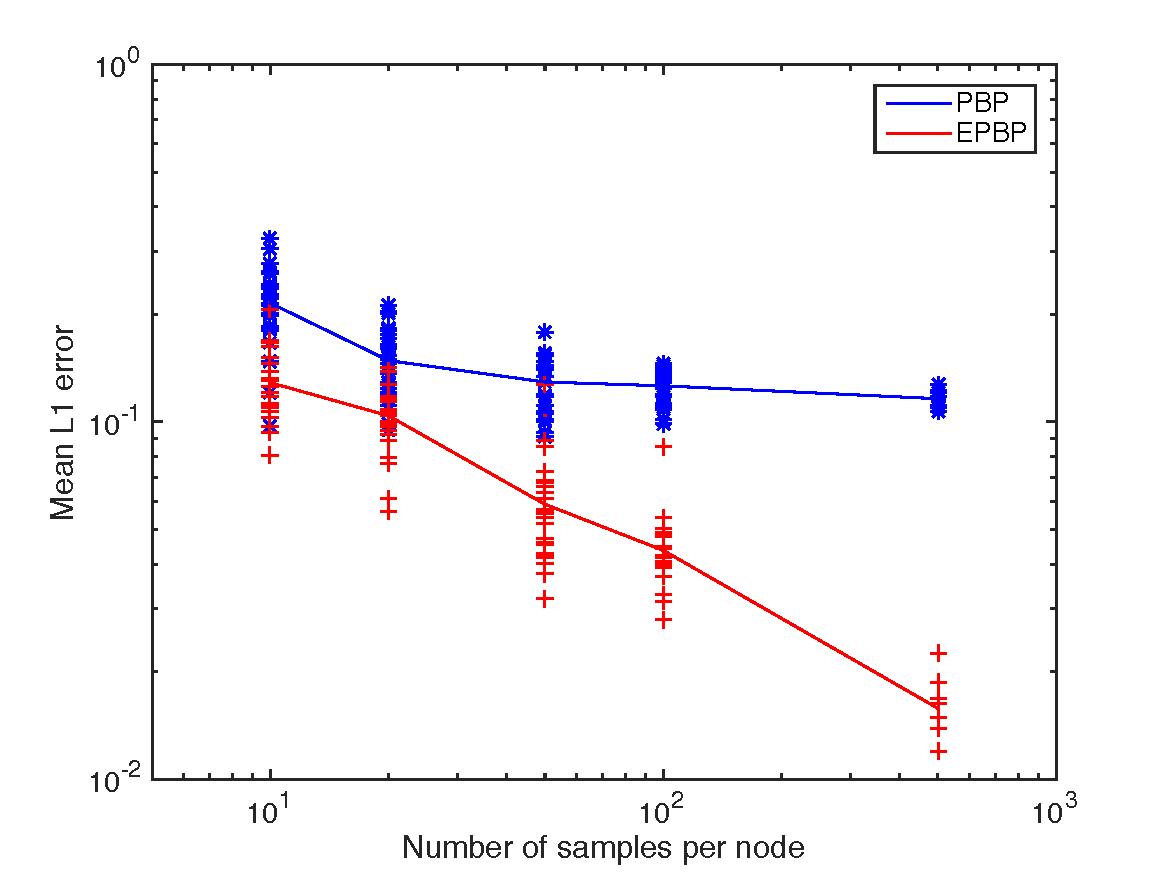
\includegraphics[width=.6\textwidth]{figures/epbp/errComparison}
%\hspace*{-.5cm}
%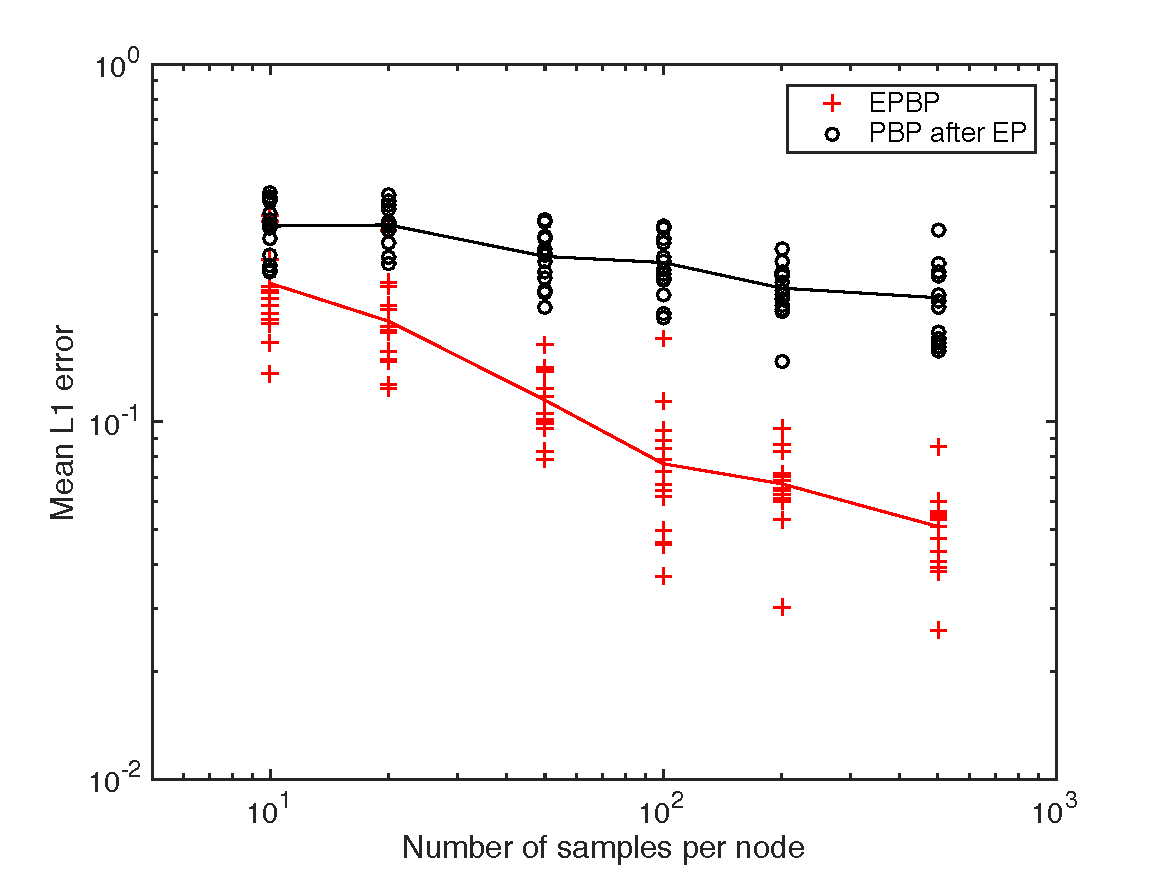
\includegraphics[scale=.35]{figures/epbp/errComparisonEP}
%\vspace*{-.3cm}
\caption{\label{figCompGrid}Comparison of the mean $L^{1}$ error for PBP and EPBP for the $3\times 3$ grid example. EPBP is more accurate for the same number of samples.} %(right) Comparison of the mean $L^{1}$ error for ``PBP after EP'' and EPBP for the tree example. In both cases, EPBP is more accurate for the same number of samples. }
\end{figure}

The \fig{compEstBelGrid} compares the estimator of the beliefs obtained by the two methods for three representative nodes (node $1$, $5$ and $9$ as illustrated in \fig{fig:grids} (left)). The figure also illustrates the last proposals constructed with our approach and one can notice that their supports match closely the support of the true beliefs.

\begin{figure}[!h]
%\vspace*{-.5cm}
\center
	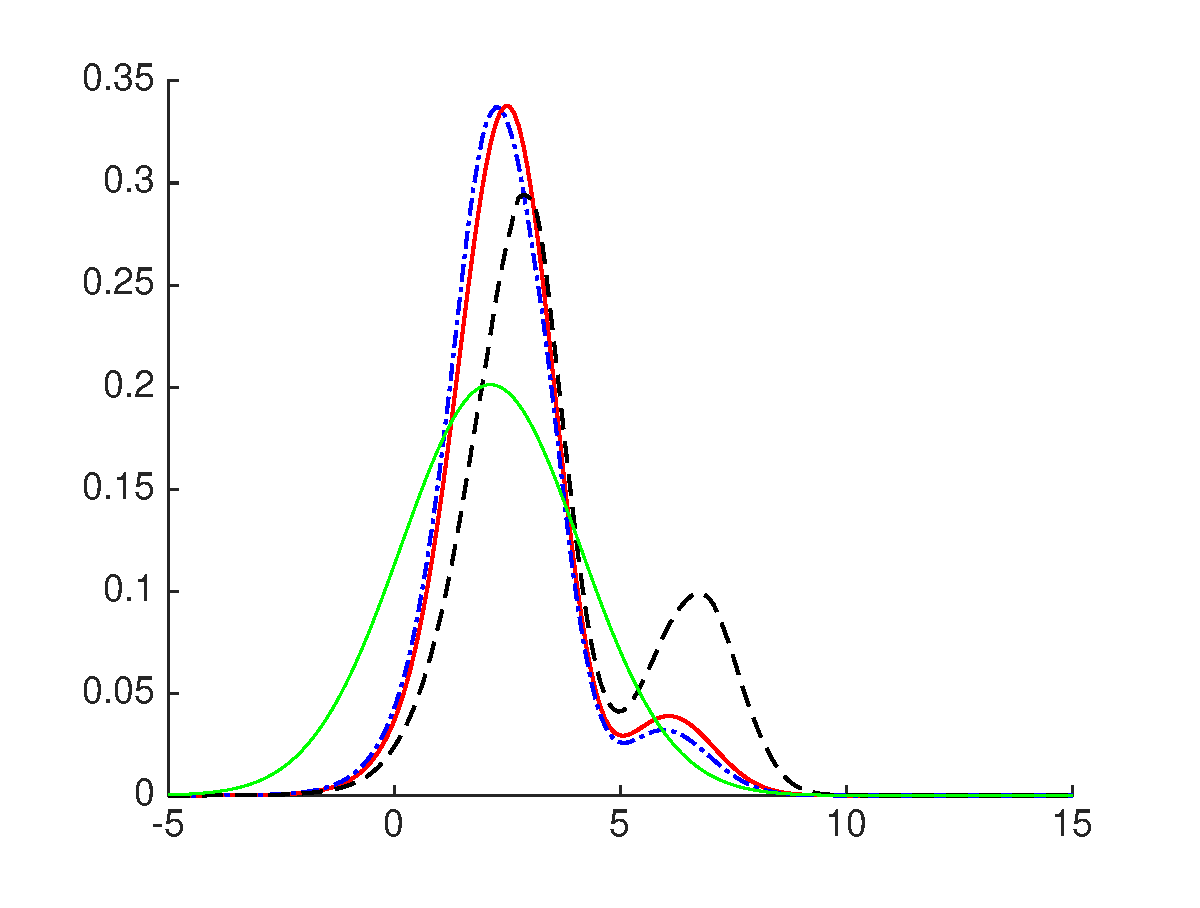
\includegraphics[width=.48\textwidth]{figures/epbp/Gnode1}
	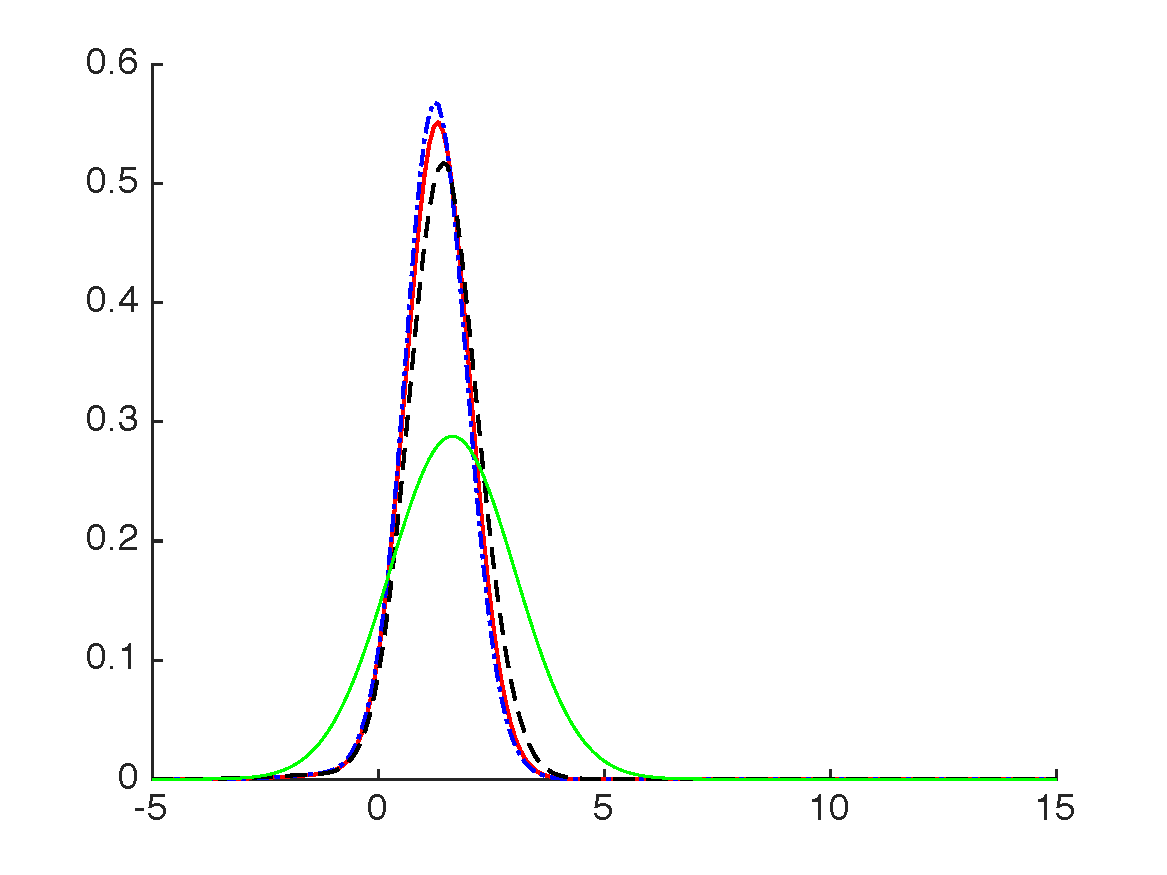
\includegraphics[width=.48\textwidth]{figures/epbp/Gnode5}
	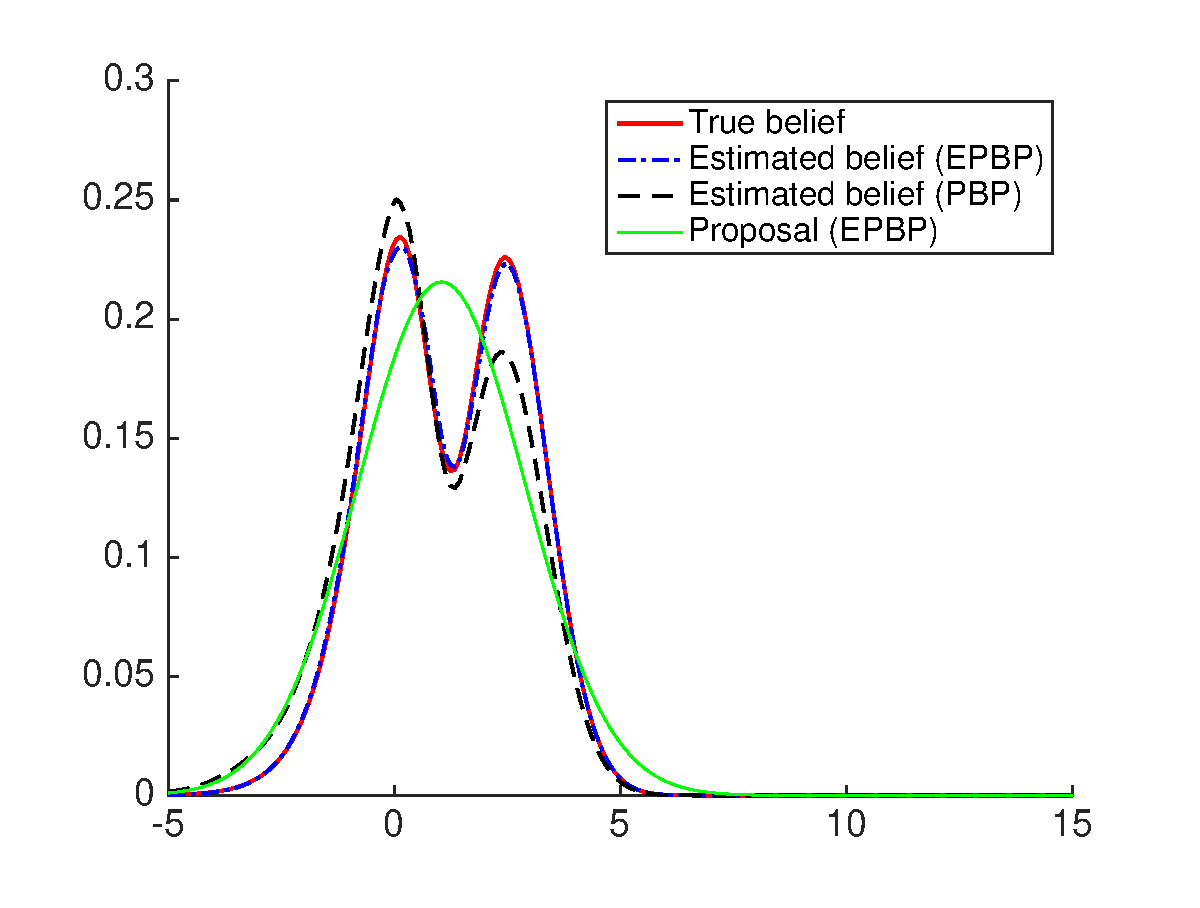
\includegraphics[width=.48\textwidth]{figures/epbp/Gnode9}
%	\vspace*{-.8cm}
%	\hspace*{-.3cm}
%	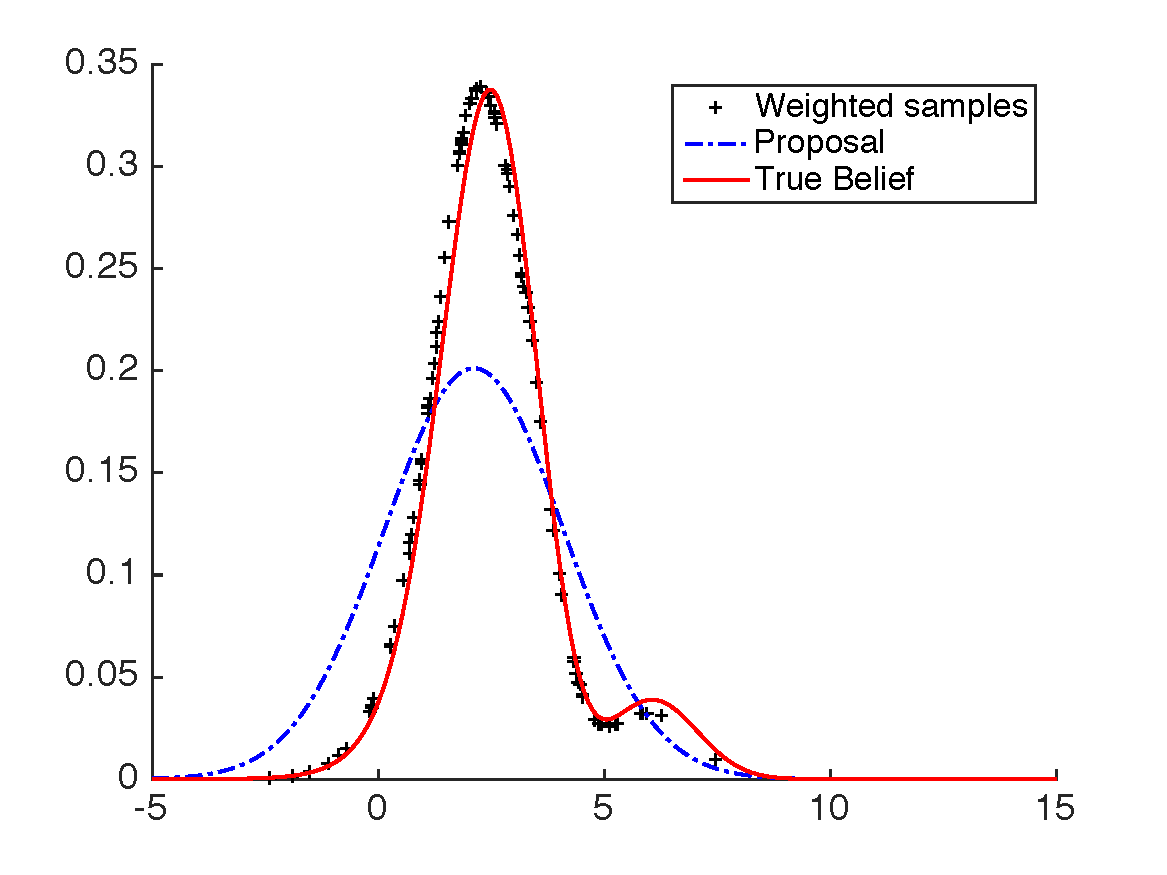
\includegraphics[scale=.25]{figs/node1_epbp}
%	\hspace*{-.5cm}
%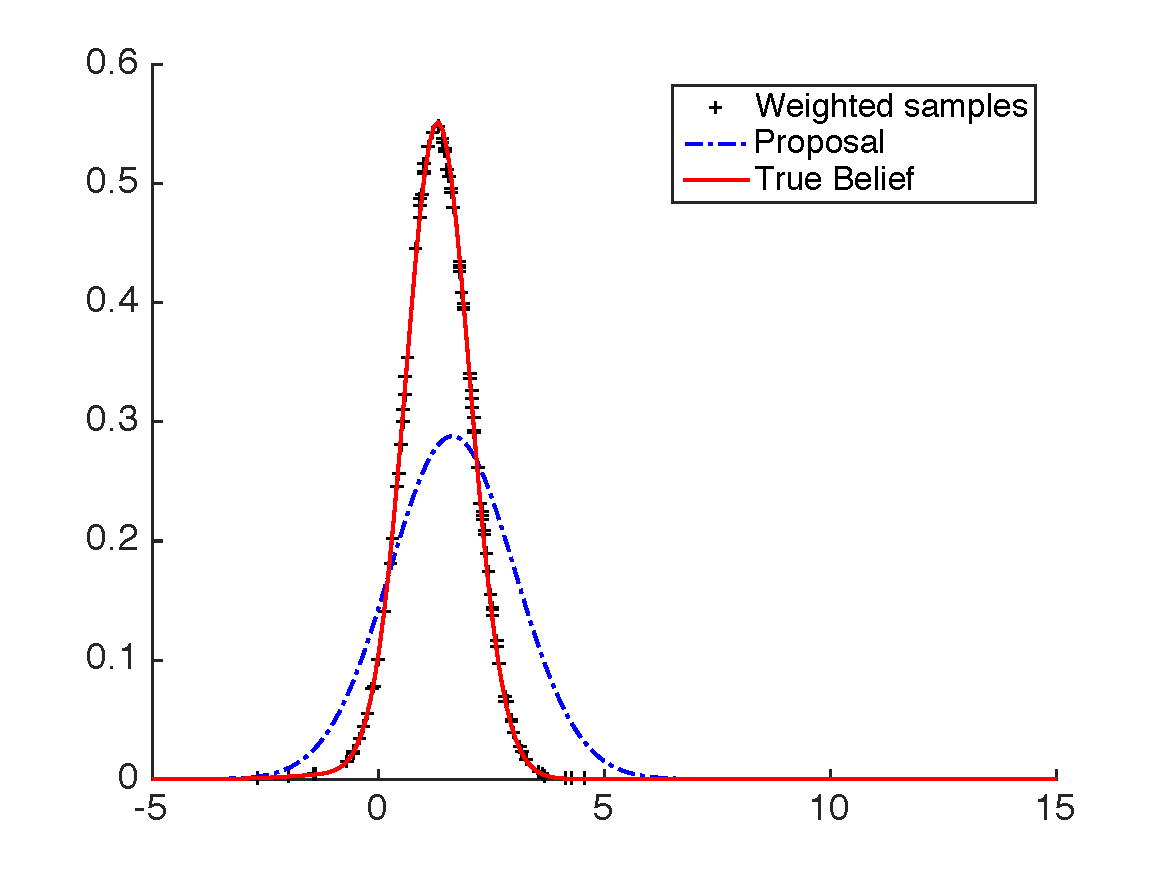
\includegraphics[scale=.25]{figs/node5_epbp}
%	\hspace*{-.5cm}
%	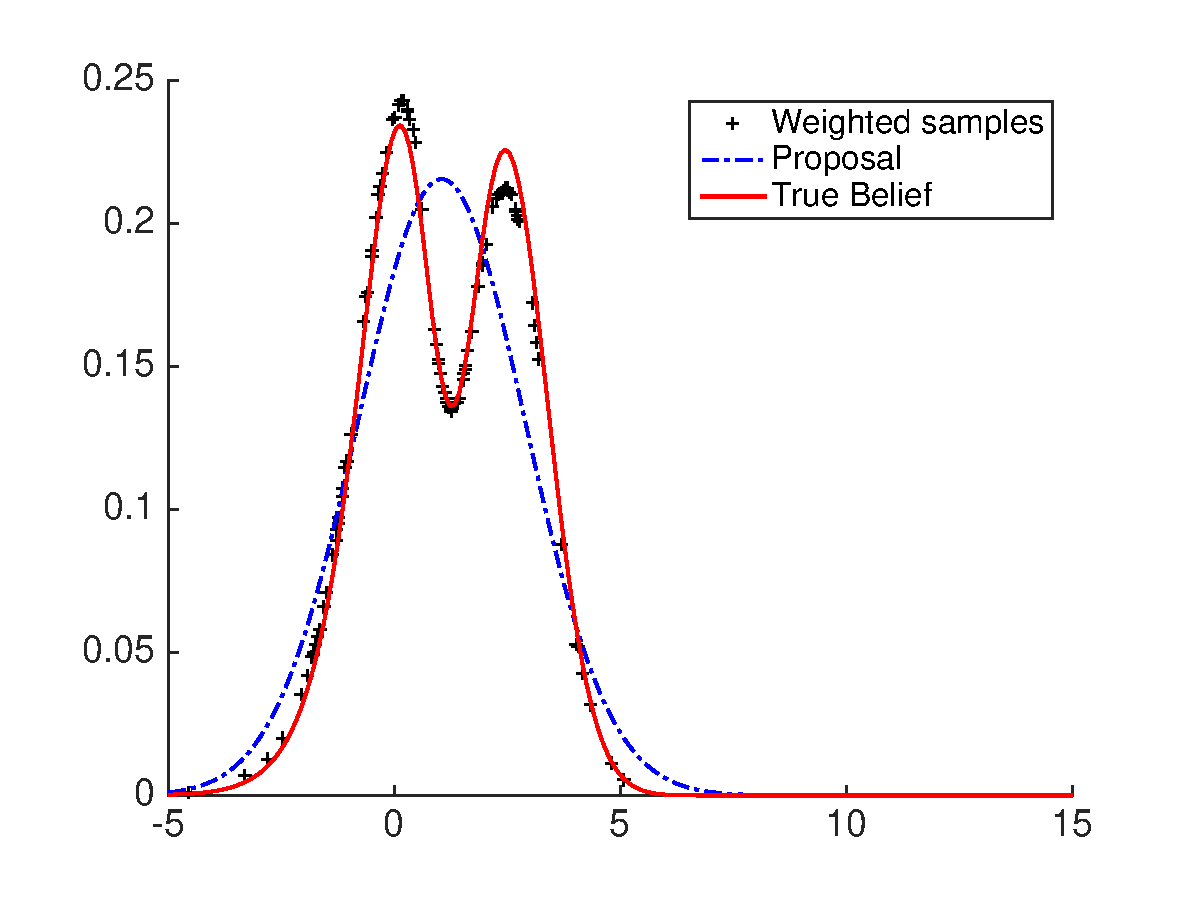
\includegraphics[scale=.25]{figs/node9_epbp}
\caption{\label{compEstBelGrid}Comparison of the beliefs on node $1$, $5$ and $9$ (top left, top right, bottom) as obtained by evaluating LBP on a deterministic mesh (\emph{true belief}), with PBP and with EPBP for the $3\times 3$ grid example. All three plots share the same legend. The proposal used by EPBP in the last step is also illustrated. The results are obtained with $N=100$ samples on each node and $20$ BP iterations. One can observe visually that EPBP outperforms PBP.}
\end{figure}

The speed-up offered by EPBP is very substantial as can be seen in \fig{compConv} (left). Hence, although it would be possible (and sensible) to use more MCMC iterations within PBP to improve its accuracy, it would make the method prohibitively expensive to use compared to EPBP. The \fig{compConv} (right) illustrates how the estimated beliefs converge as compared to the true beliefs with increasing number of loopy belief propagation iterations. One can observe that PBP converges more slowly and that the results display more variability which is likely also due to the MCMC runs being too short. %Making them longer is unpractical however as the computational complexity is already higher than that of EPBP.

%
%
%%\newpage
%
%
%
%% THIS IS from THE /DATAMIXNG/ folder

%
\begin{figure}[!h]
\center
%\vspace*{-.5cm}
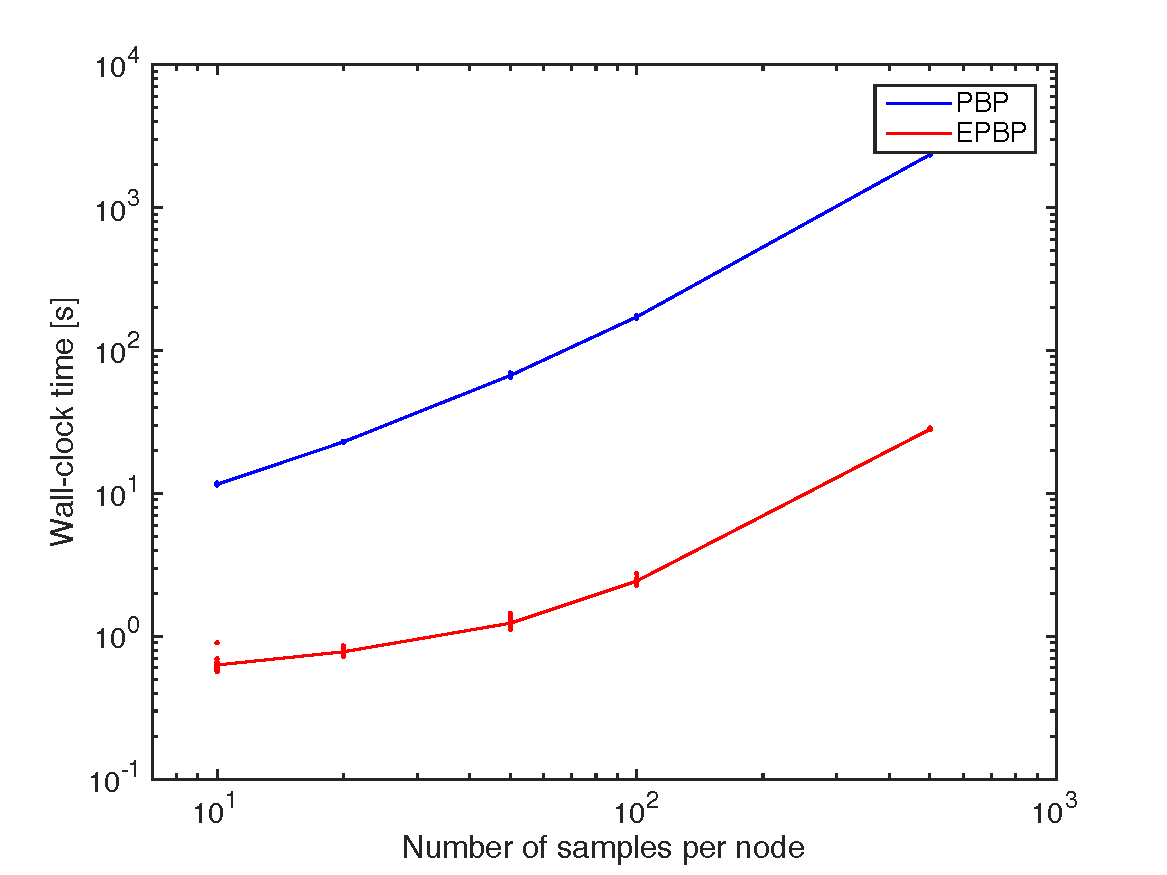
\includegraphics[width=.51\textwidth]{figures/epbp/timeComparison}
\hspace*{-.7cm}
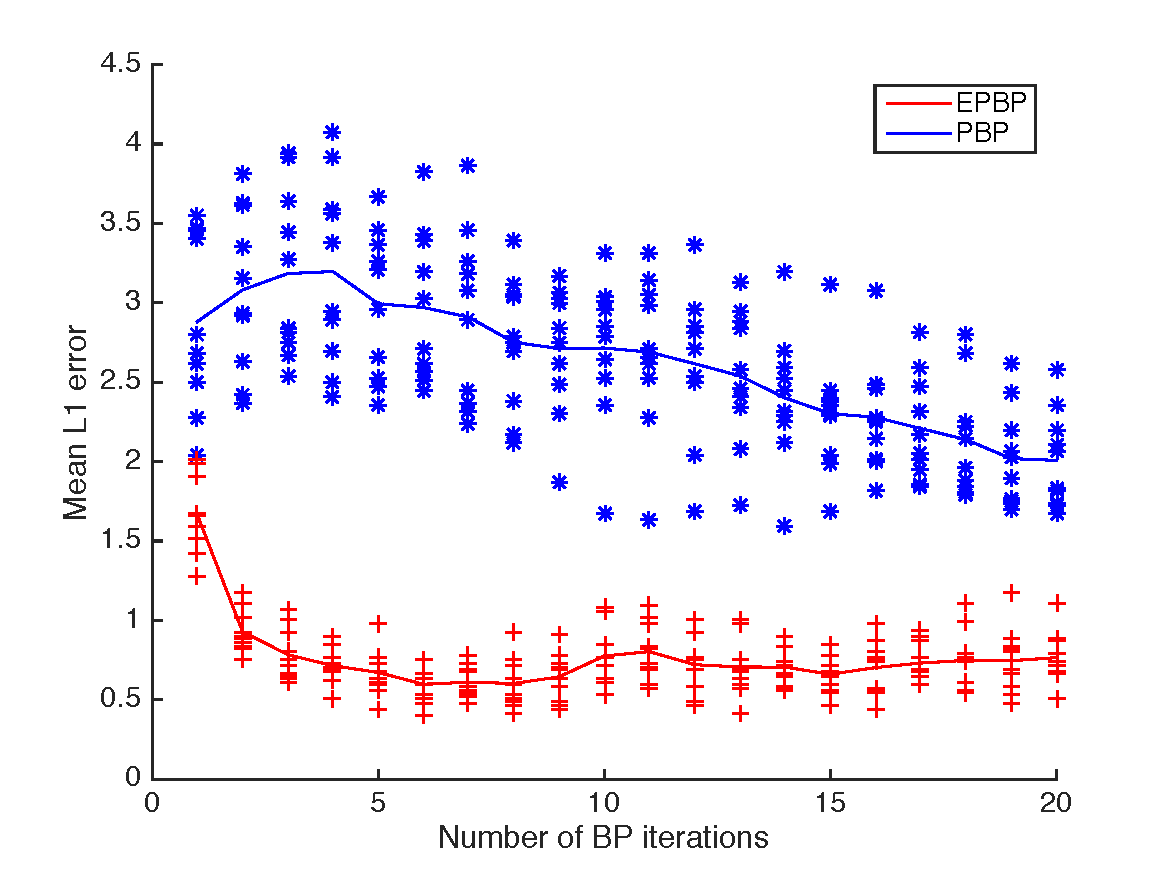
\includegraphics[width=.51\textwidth]{figures/epbp/compBPconv}
%
%\vspace*{-.4cm}
\caption{\label{compConv} Comparison of the convergence in $L^{1}$ error with increasing number of BP iterations for the $3\times 3$ grid when using $N=30$ particles. }%(right) Comparison of the wall-clock time needed to perform PBP and EPBP on the $3\times 3$ grid example.}
\end{figure}
%
%
%\newpage
%
The same experiments were also run on the tree example with similar results.
Additionally, we looked at how ``pure EP'' with normal distributions performs. We also tried using the distributions obtained with EP as proposals for PBP (referred to as ``PBP after EP'' in figures). All those methods underperform compared to EPBP. In particular one can observe in \fig{compPBPaEP} that ``PBP after EP'' converges slower than EPBP with increasing number of samples.
%
%
%
\begin{figure}[!h]
\center
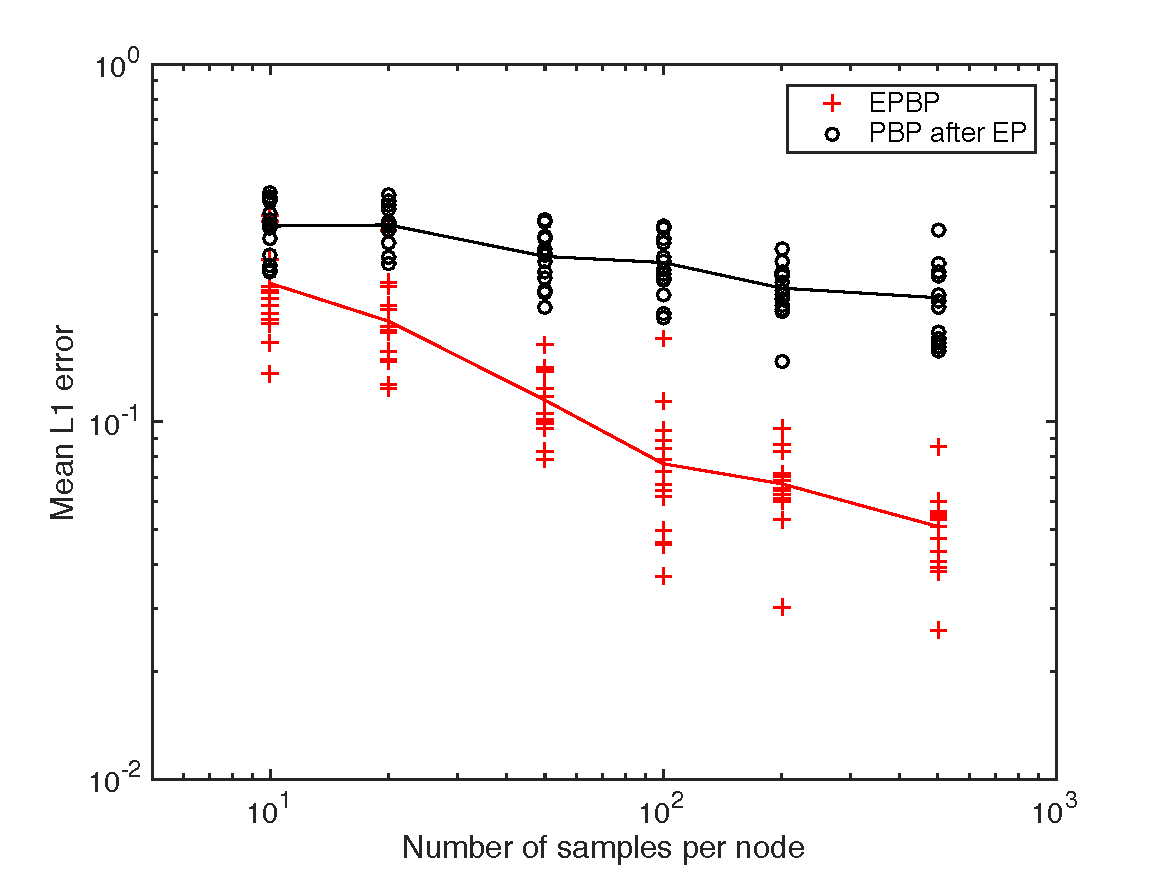
\includegraphics[width=.6\textwidth]{figures/epbp/errComparisonEP}
\caption{\label{compPBPaEP}Comparison of the mean $L^{1}$ error for EPBP and ``PBP after EP'' for the tree example. EPBP is more accurate and converges faster.}
\end{figure}


The \fig{compTree} compares the estimator of the beliefs obtained by all the methods on the tree example for three representative nodes (node $1$, $3$ and $8$ as illustrated in \fig{fig:grids} (right)). As for the grid example, the figure illustrates how EPBP better recovers the true beliefs. 


\begin{figure}[!h]
\center
%\vspace*{-.2cm}
%	\hspace*{-.3cm}
	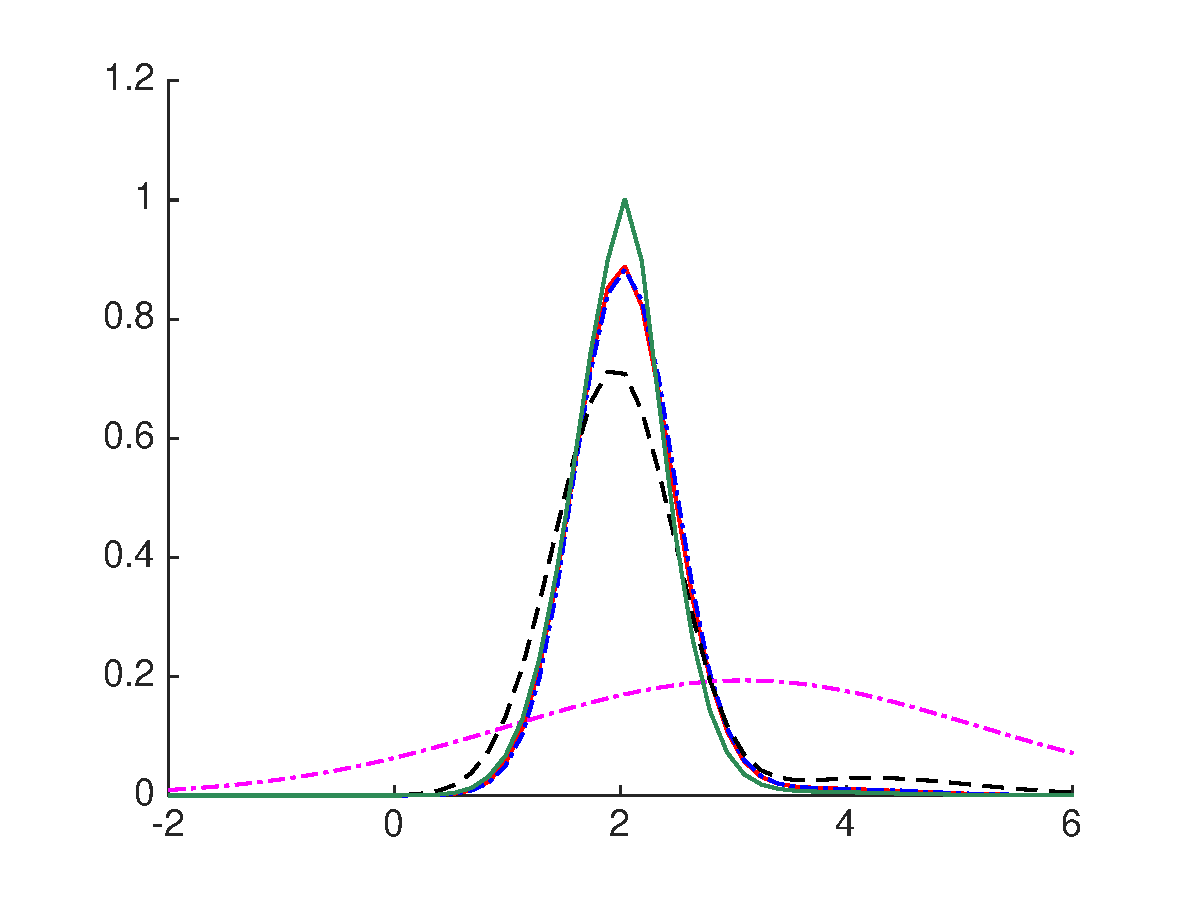
\includegraphics[width=.48\textwidth]{figures/epbp/tree_node1}
%	\hspace*{-.5cm}
	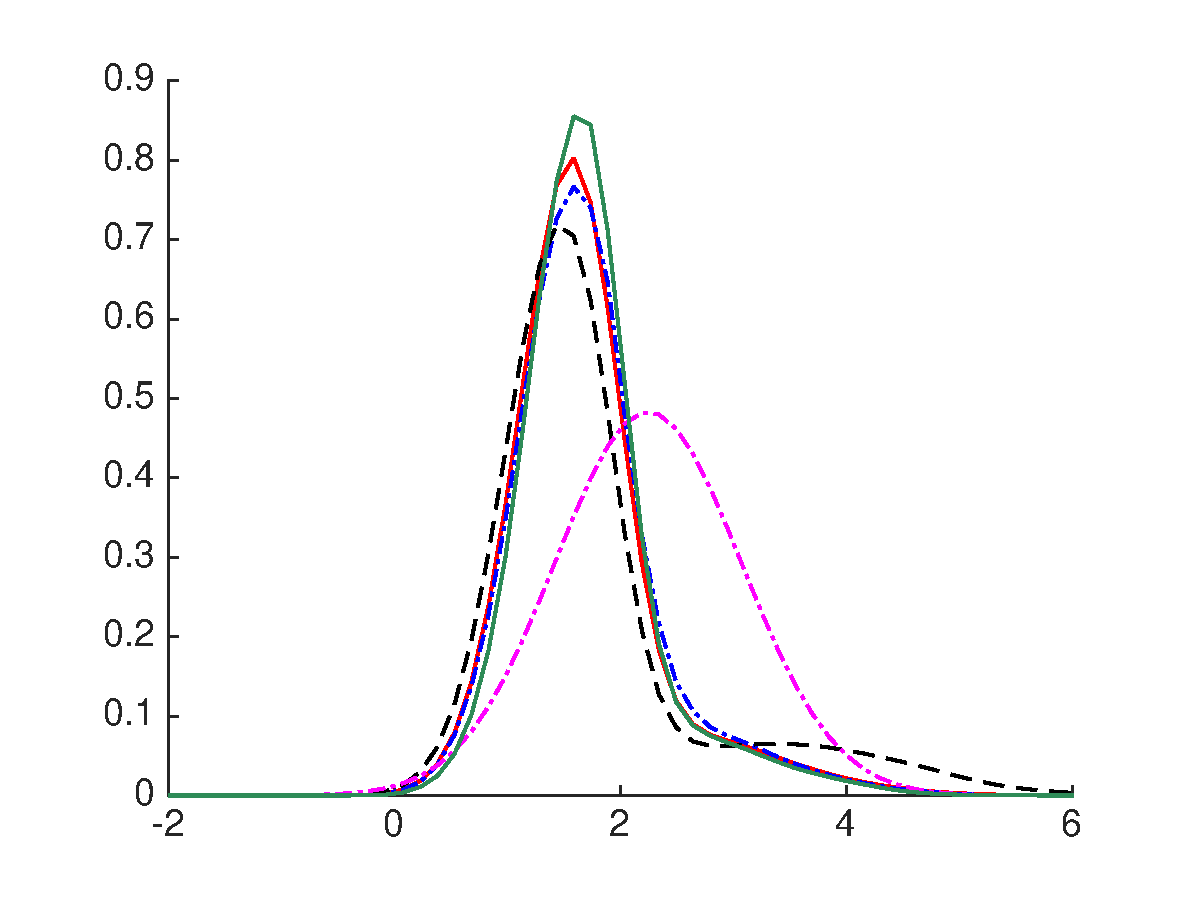
\includegraphics[width=.48\textwidth]{figures/epbp/tree_node3}
%\hspace*{-.5cm}
	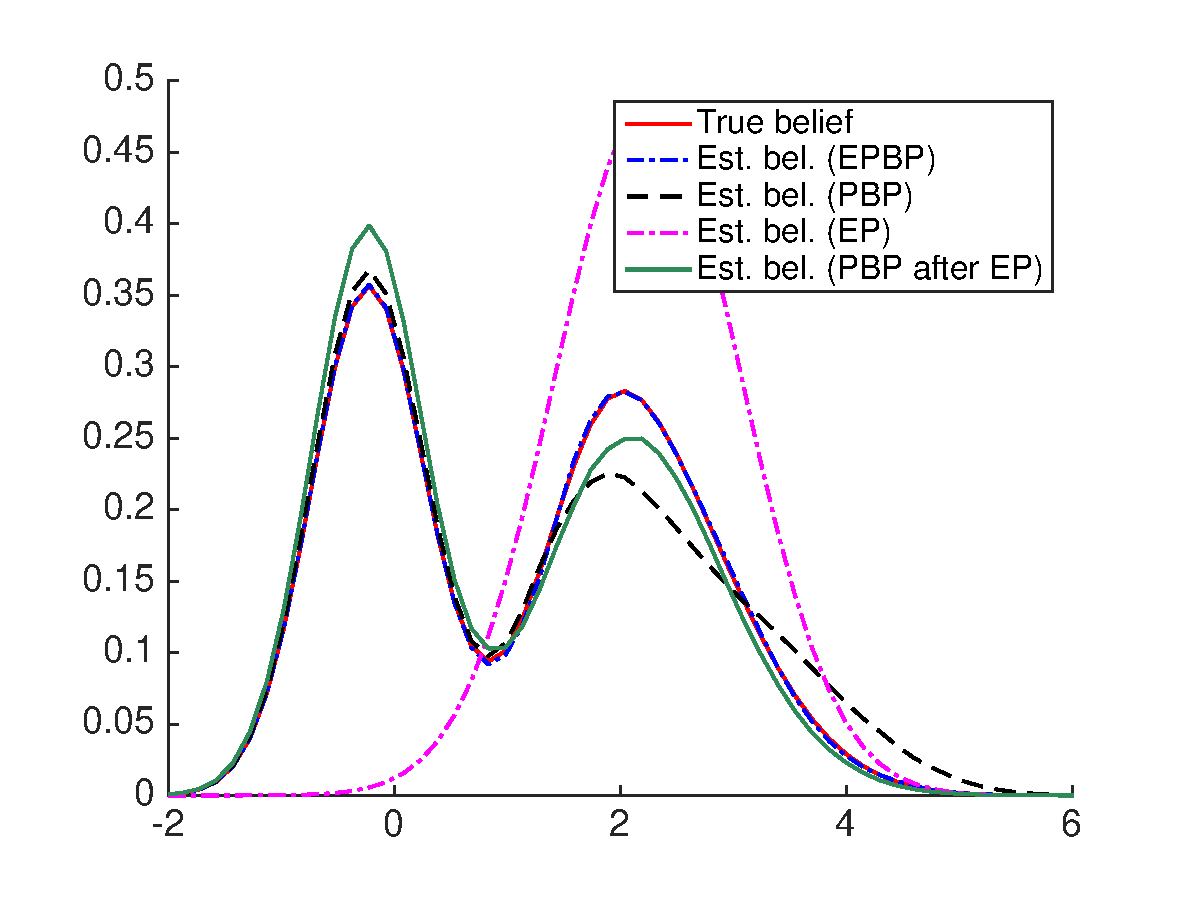
\includegraphics[width=.48\textwidth]{figures/epbp/tree_node8}

	\caption{\label{compTree}Comparison of the beliefs on node $1$, $3$ and $8$ (top left, top right, bottom) as obtained by evaluating LBP on a deterministic mesh, using EPBP, PBP, EP and PBP using the results of EP as proposals. All three plots share the same legend. This is for the tree example with $N=100$ samples on each node and $20$ LBP iterations. Again, one can observe visually that EPBP outperforms the other methods. }
\end{figure}

\subsection{Sub-quadratic implementation and denoising application}
As outlined at point \ref{sec:EPBP-compcompl}, the inherent quadratic complexity of the EPBP algorithm can be reduced to $\mathcal O(MN)$ where $M$ is the number of mixture components effectively considered to represent the messages. 
We apply this method to the $3\times 3$ grid example in the case where $M=\mathcal O(\log(N))$: for $N=\{10,20,50,100,200,500\}$, we pick $M=\{5, 6,8,10,11,13\}$. The results are illustrated in \fig{figCompNLOGN} where one can see that the $N\log N$ implementation compares very well to the original quadratic implementation at a much reduced cost. We apply this sub-quadratic method on a simple probabilistic model for an image denoising problem. The aim of this example is to show that the method can be applied to larger graphs and still provide good results. The model underlined is chosen to showcase the flexibility and applicability of our method in particular when the edge-potential is non-integrable. It is not claimed to be an optimal approach to image denoising.\footnote{In this case in particular, an optimization-based method such as that of \citet{rudin92} is very likely to yield better results and much faster.} \\
The node and edge potentials are defined as follows:
\eqa{	
	\left\{
		\begin{array}{lcl}
			\psi_{u}(x_{u}) &=& \mathcal N(x_{u}-y_{u};0,0.1)\\
			\psi_{uv}(x_{u},x_{v}) &=& \mathcal L^{\lambda}(x_{u}-x_{v};0,0.03)
		\end{array}
	\right.,\label{modelIMG}
}
where $\mathcal L^{\lambda}(x;\mu,\beta)=\mathcal L(x;\mu,\beta)$ if $|x|\le \lambda$ and $\mathcal L(\lambda;\mu,\beta)$ otherwise. In this example we set $\lambda=0.2$. The value assigned to each pixel of the reconstruction is the estimated mean obtained over the corresponding node (figure \ref{figIMG}). The image has size $50\times 50$ (therefore corresponding to a grid graph of 2500 nodes) and the simulation was run with $N=30$ particles per nodes, $M=5$ and $10$ BP iterations taking under 2 minutes to complete. We compare it with the result obtained with EP on the same model. Note that running PBP on this example would be unrealistic due to the size of the underlying graph.


\begin{figure}[!h]
%\vspace*{-.7cm}
\center
%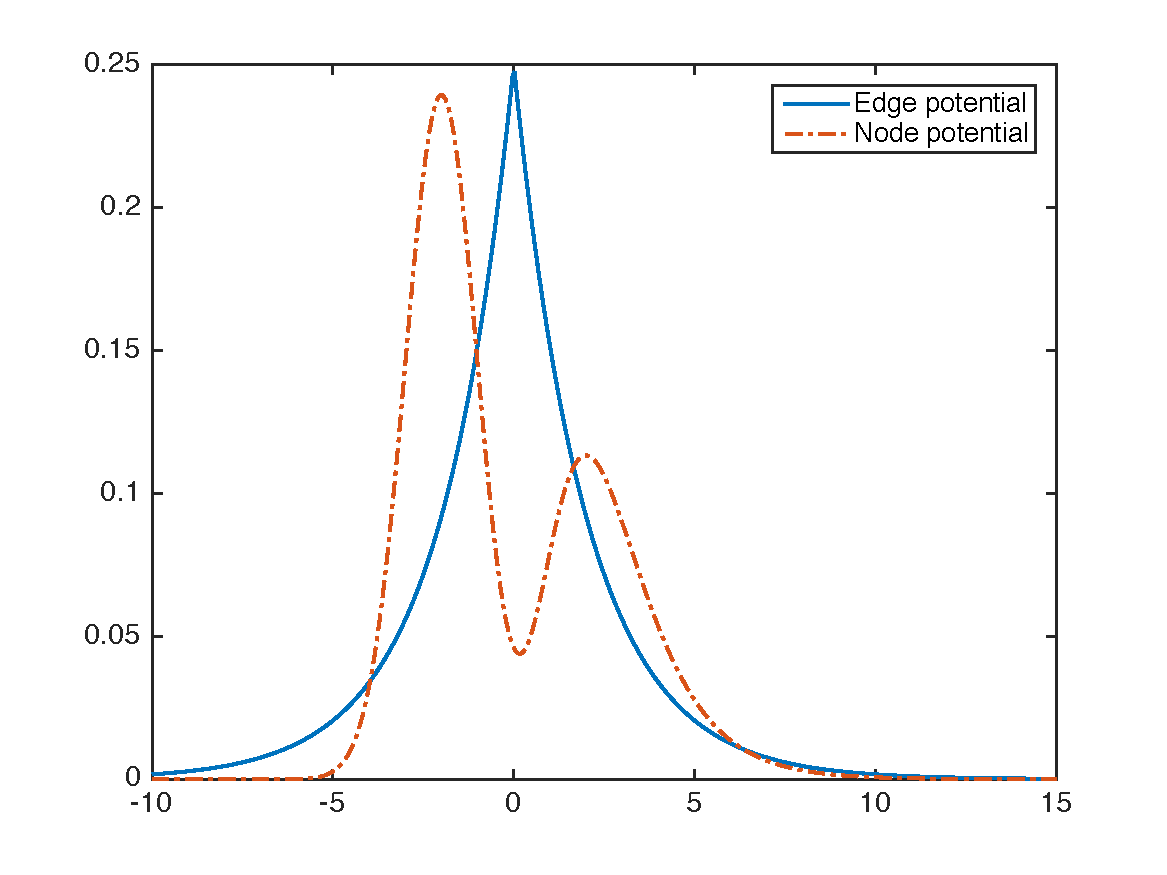
\includegraphics[scale=.25]{figs/node_edge_pot}
%\hspace*{-.6cm}
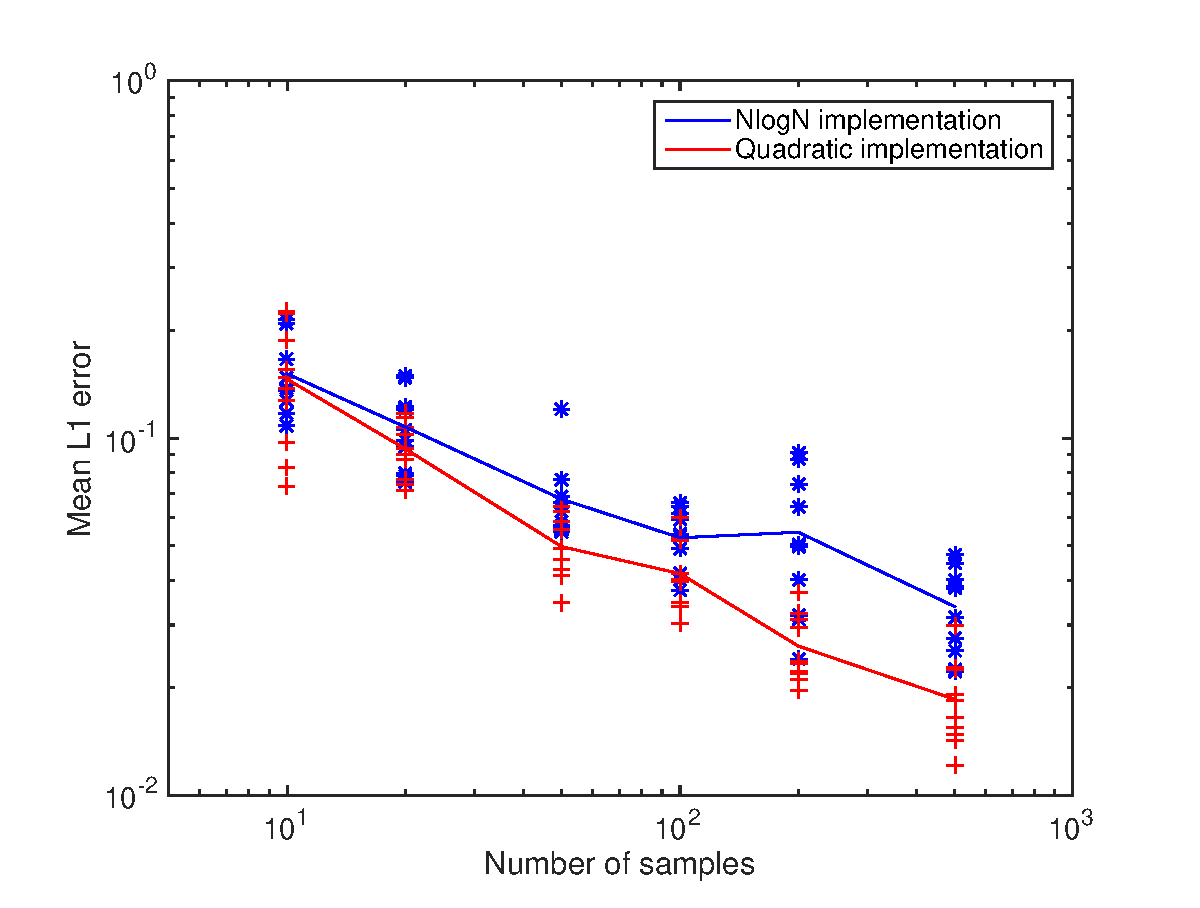
\includegraphics[width=.51\textwidth]{figures/epbp/errCompNLOGN}
\hspace*{-.7cm}
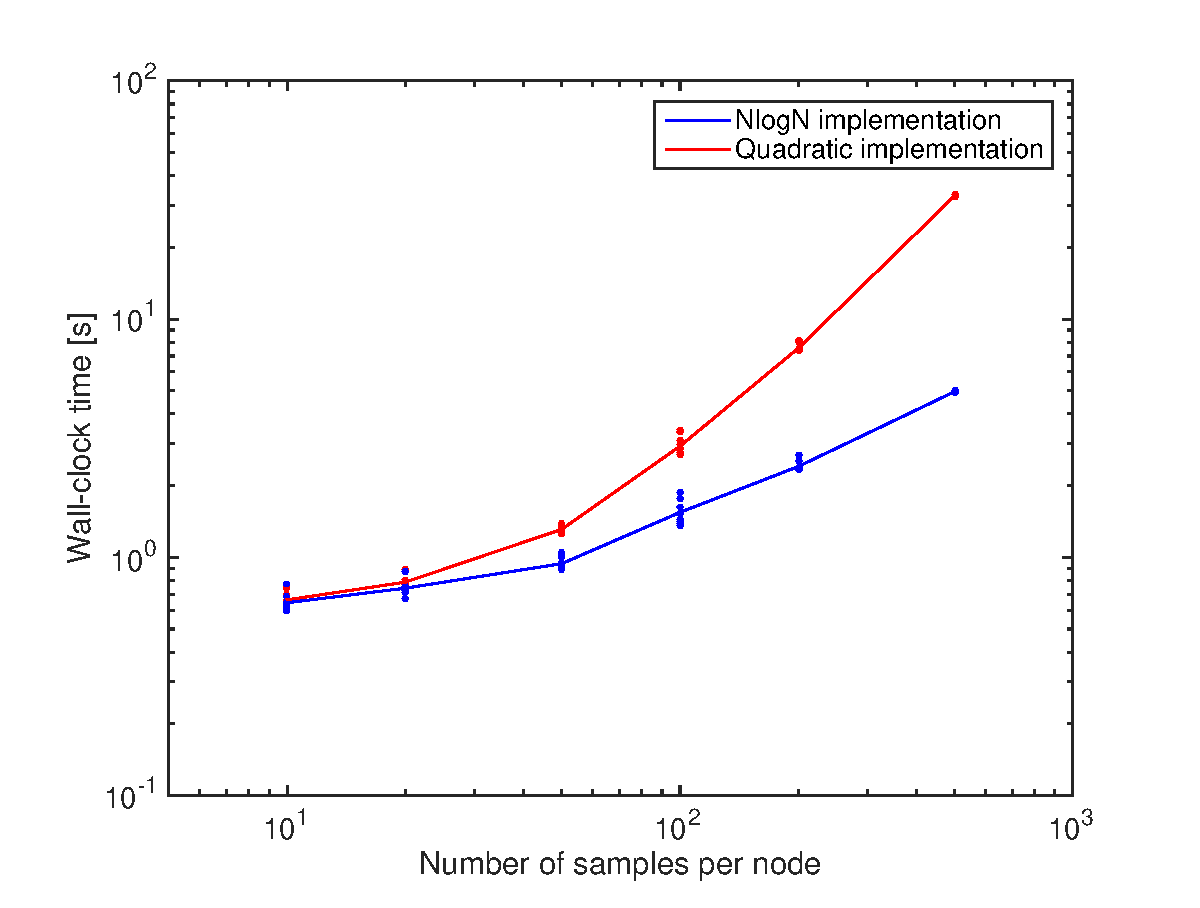
\includegraphics[width=.51\textwidth]{figures/epbp/timeCompNLOGN}
%\vspace*{-.4cm}
\caption{\label{figCompNLOGN}Comparison of the quadratic and $\mathcal O(N log N )$ implementations. (left) Comparison of the mean L1 error, (right) comparison of the wall-clock time. The sub-quadratic implementation performs almost as well as the original implementation and offers a significant speedup.}


\end{figure}
\begin{figure}[!h]
\center
%\hspace*{-2cm}
%\vspace*{-.4cm}

\includegraphics[scale=.25]{figures/epbp/denoisingExpleORIG}
\hspace*{.3cm}
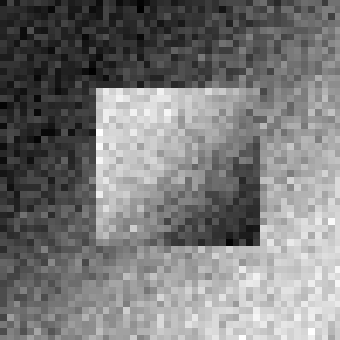
\includegraphics[scale=.25]{figures/epbp/denoisingExpleINPUT}
\hspace*{.3cm}
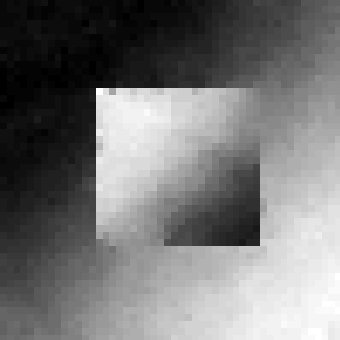
\includegraphics[scale=.25]{figures/epbp/denoisingExpleRECO}
\hspace*{.3cm}

\includegraphics[scale=.25]{figures/epbp/denoisingEP2}
%\hspace*{-1.5cm}
%\vspace*{-.3cm}
\caption{\label{figIMG} From left to right: comparison of the original (first), noisy (second) and recovered image using the sub-quadratic implementation of EPBP (third) and with pure EP (fourth). % with $N=30$ samples per nodes and $10$ BP iterations with the model \eqref{modelIMG}.
}
\end{figure}

% >>>>>>>>>>>>>>>>>>>>>>>>>>>>>>
% >>>>>>>>>>>>>>>>>>>>>>>>>>>>>>
% >>>>>>>>>>>>>>>>>>>>>>>>>>>>>>
% >>>>>>>>>>>>>>>>>>>>>>>>>>>>>>

%%%%%%%%%%
\section{Discussion}

\todofr{
\begin{itemize}
\item watch out to not stress consistency for subquad algo (consistency probably incorrect anyway as per conversation with Naesseth)
\item discuss existing, PBP, NBP etc. explain that NBP probably good for most cases (?) a little bit like KF for HMM.
\item add here or otherwise
\end{itemize}
}\fi

\chapter[EP for Distributed Bayesian Inference]{Expectation Propagation for\\ Distributed Bayesian Inference}
\ifsnep% !TEX root = ../thesis.tex

\todofr{
	\begin{itemize}
		\item Geometry and KL and mirror descent
		\item trick of the trade when projections don't work and why
	\end{itemize}
}

%%%%%%%%%%%%%%%%%%%%%%%%%%%%%%%%%%%%%%%%
\section{Distributed Bayesian inference}

In this section we consider the problem of performing Bayesian inference when the relevant data is distributed across different compute nodes. 
Let us assume that there are $K$ such compute nodes each holding independent parts of the data $y_i$ (with $i=1,\dots,K$) such that these parts form a partition of the complete data $y$. 
In a Bayesian setting, we are interested in the posterior distribution over a parameter of interest $x$ given the entire data $y$. We can write this posterior as the product of $K$ terms corresponding to the parts $y_i$: \check{june8}
%
\eqa{
	p(x\st y) &\propto& \pi_0(x) \prod_{i=1}^{K} p(y_i\st x)\label{eq:distrposterior}
}
%
where $\pi_0$ is a prior distribution. Each of the likelihood term itself factors over the individual data points of $y_i$, i.e.: $p(y_i\st x)=\prod_{j=1}^{N_i}p(y_{ij}\st x)$ with $N_i$ the number of individual data points held by the compute node $i$.

\todofr{Add here litt, why is this relevant, some basic stuff that have been tried + references}

Defining $t_i$ to be nonnegative factors with $t_i(x)=p(y_i\st x)$, the factorised form \eqref{eq:distrposterior} reads $\pi_0(x)\prod_{i=1:K}t_i(x)$ which is the form \eqref{eq:targetfactorises} that we had used to motivate the introduction of the ADF and EP algorithms (cf.\ point \ref{s:ADF+EP}).
In the rest of this chapter, we show how different variants of the EP algorithm can be used to perform parallel variational inference in the presence of distributed data.\check{jun8} 

\add{come back to this, add litt for distr bayesian (see SNEP paper), see also confirmation}

%%%%%%%%%%%%%%%%%%%%%%%%%%%%%%%%%%%%%%%%%%%%%%%
\section{EP variants for distributed inference}
As indicated in the introductory point, we consider a target distribution of the form $p(x)\propto \pi_0\prod_{i=1:K}t_i(x)$ where the evaluation of one of the $t_i$ requires access to the compute node $i$. The aim is to construct an approximation $q\in\mathcal F_\phi$ parametrised by a vector $\theta$ with
%
\eqa{
	q(x) &=& \pi_0(x)\exp(\scal{\theta,\phi(x)}-A(\theta)) \spe \pi_0(x)\exp(-A(\theta))\prod_{i=1}^{K}\tilde t_i(x)
}
%
where $\tilde t_i(x):=\exp\scal{\omega_i,\phi(x)}$, and therefore: $\sum_{i=1:K}\omega_i=\theta$. The tilted distributions associated with each of the factors are given by
%
\eqa{
	q_i(x) &=& \pi_0(x)t_i(x)\exp(\scal{\lambda_i,\phi(x)}-A_i(\lambda_i))
}
% 
where $\lambda_i=(\theta-\omega_i)$ and $A_i(\lambda_i)$ is the corresponding log-partition function. Much like the log-partition function of $q$, the $A_i$ are convex and $\nabla A_i(\lambda_i)=\E_{q_i}[\phi(X)]$. Indeed, each $A_i$ is simply the log-partition functions of the exponential-family $\mathcal F_\phi$ with respect to a modified base-measure including $t_i$.
In the EP setting, we seek to determine the parameters $\omega_1,\dots,\omega_K$ such that the LMMC \eqref{eq:LMMC} hold, i.e.: $\E_q[\phi(X)]=\E_{q_i}[\phi(X)]$ for each $i=1,\dots,K$.
The general parallel computational framework considered iterates on the following steps:
\begin{enumerate}\itsepa
	\item the master node sends a global parameter $\theta$ to each compute node,
	\item each compute node $i$ attempts to find a new $\omega_i$ such that the corresponding LMMC is (approximately) met and sends the updated $\omega_i$ to the master node,
	\item the master node integrates the new $\omega_i$ into $\theta$.
\end{enumerate} 

As we will see, there are different ways to implement this general framework.
We will show empirically that a determining element in the performance of a particular implementation is its robustness to Monte Carlo noise. 
Indeed, in our general setting we do not assume that computing $\E_{q_i}[\phi(X)]$ can be done exactly. Rather, we assume that it is approximated by a Monte Carlo estimator.\check{june8}
%%%%%%%%%%%%%%%%%%%%%%%%%%%%%%%%%%%%%%%%%%%%%%%%%%%%%%%%%
\subsection{Damped updates in the natural parameter space}
In their paper, \citet{xu14} suggest a method to synchronise Monte Carlo samplers ran on independent compute nodes. They call it \emph{Sequential Moment Sharing} or SMS for short. Effectively, SMS corresponds precisely to the case mentioned at the previous point consisting of running EP across multiple physical nodes while using noisy estimates of $\E_{q_i}[\phi(X)]$, the expected value of the sufficient statistics under the tilted distribution. 
Below, we introduce the algorithm as a damped fixed-point iteration in the natural parameter space. This will prove useful when comparing different EP-like algorithms.\check{june8,may27}\\

We showed that the basic EP algorithm could be interpreted as a kind of fixed point iteration targeting the Local Moment Matching Conditions \eqref{eq:LMMC} (LMMC). At a given step of the algorithm, when considering the inclusion of the factor $t_i$, the global parameter should therefore be updated such as to verify $\E_{q_\theta}[\phi(X)]= \E_{q_i}[\phi(X)]$. Let $\mu_i:=\E_{q_i}[\phi(X)]$, the update then amounts to finding $\theta$ such that $\nabla A(\theta) = \mu_i$ or
%
\eqa{	
	\theta &\leftarrow & \nabla A^{\star}(\mu_i).	\label{eq:ep-np-update}
}
%
In the case where one is considering a Monte Carlo estimator for $\mu_i$, these updates are inexact and it is crucial to mitigate the effect of the noise by considering \emph{damped updates}.\add{would be good to come back further to this when considering the gaussian case (inversion of noisy matrix), mention it in discussion} In fact, even when one uses the exact $\mu_i$, it can be beneficial to the overall convergence of the algorithm to consider damped updates \citep{heskes03}. Damping \eqref{eq:ep-np-update} leads to the modified update:\check{may11}
%
\eqa{
	\theta &\leftarrow & (1-\kappa)\theta + \kappa \nabla A^{\star}(\hat\mu_i),\label{eq:damped-update-np}
}
%
where $\kappa \in(0,1]$ is the damping parameter and $\hat\mu_i$ is an estimator for $\mu_i$. As in the gradient descent algorithm, the damping parameter can be decreased over iterations according to a schedule in order to further help convergence.\add{We will explore the connection to GD in more details later}
The damped update \eqref{eq:damped-update-np} can also be expressed in terms of the $\omega_i$ (parameter of the factor approximation $\tilde t_i$) and the $\lambda_i$ (parameter of the corresponding cavity):\check{june8}
%
\eqa{
	\omega_i &\leftarrow& \omega_i + \kappa(\nabla A^{\star}(\hat\mu_i)-\lambda_i).\label{eq:damped-update-np-w}
}
%
One can also swap the role of $\lambda_i$ and $\omega_i$ and obtain another valid damped update mechanism. Both forms are amenable to parallelisation since they can be expressed solely in terms of local parameters attached to the $i$th compute node.\add{review statement, potentially in lambdai less stable because cavity collapse but should check if can explain why}\check{june8,may27}\\

The basic SMS algorithm operates synchronous updates.
At step $k$, each node receives the current global parameter $\theta$ and computes the parameter corresponding to the current tilted distribution $q_i$ i.e.: $\lambda_i=(\theta-\omega_i)$. Each node then forms a Monte Carlo estimator $\hat\mu_i$ of $\E_{q_i}[\phi(X)]$, computes the damped step \eqref{eq:damped-update-np-w} and returns the updated local parameter $\omega_i$ to the master node. 
The master node then aggregates all updated local parameters and updates the global parameter: 
%
\eqa{	\theta &\leftarrow& (1-\kappa')\theta+\kappa'\sum_{i=1}^{K}\omega_{i}	}
%
where $\kappa' \in (0,1]$ is a global damping parameter which may also help convergence. 
These steps are summarised at the algorithm \ref{alg:ep-sms-synch} below.\check{june8}

\begin{algorithm}[!h]\small
	\caption{\label{alg:ep-sms-synch}\dblue{\emph{\small Sequential Moment Sharing (synchronous)}}}
	\begin{algorithmic}[1]
	\State Initialise $\theta,\omega_{1},\dots,\omega_{K}$ such that $\theta=\sum_{i=1}^{K}\omega_{i} \in \Omega$ and send to each compute node
	\For{$k=1:N_{\text{EP}}$}
		\State Send current global parameter $\theta$ to each node
		\For{node $i=1:K$}
			\State Update the cavity parameter $\lambda_{i}\leftarrow\theta-\omega_{i}$
			\State Form an estimator $\hat\mu_{i}$ of $\E_{q_{i}}[\phi(X)]$
			\State Update the local parameter $\omega_{i}\leftarrow\omega_{i}+\kappa(\nabla A^{\star}(\hat\mu_{i})-\lambda_i)$
			\State Send the updated $\omega_{i}$ to the master node
		\EndFor
		\State Update global parameter $\theta\leftarrow (1-\kappa')\theta + \kappa'\sum_{i=1}^{K}\omega_{i}$
	\EndFor\\	
	\Return{$\theta$}
	\end{algorithmic}
\end{algorithm} 

It is easy to see how this algorithm can be altered to accommodate asynchronous updates. Indeed, instead of waiting for all nodes to complete their tasks, each node could asynchronously request the most recent $\theta$ available from the master node while the master node would continuously integrate information it receives from the compute nodes. In fact, each node would then simply send the difference $\delta_{i} = (\omega_{i}^{\text{new}}-\omega_{i}^{\text{old}})$ which can be integrated directly into an update of $\theta$. \check{june8}

%%%%%%%%%%%%%%%%%%%%%%%%%%%%%%%%%%%%%%%%%%%%%%%%%%%%%%%%%
\subsection{Damped updates in the mean parameter space}

The main issue with the SMS algorithm which we will expose in more details in the experiments\add{do it and refer} is that it performs the projection of the noisy estimator $\hat\mu_{i}$ \emph{before} the damping step. Since this projection operator is likely non-linear and potentially numerically unstable this can hinder the performances of the algorithm. In the case of the Gaussian distribution for instance, the projection effectively requires the inversion of a noisy matrix (see \eqref{proj-mp-np-gauss}). It seems therefore sensible to suggest damping the estimator \emph{before} it gets projected. This leads to going from \eqref{eq:damped-update-np} to\check{june11}
%
\eqa{
\nabla A(\theta) &\leftarrow& (1-\kappa)\nabla A(\theta) + \kappa \hat\mu_{i}
}
%
or, equivalently, to
%
\eqa{
\theta &\leftarrow& \nabla A^{\star}(\nabla A(\theta) + \kappa (\hat\mu_{i}-\nabla A(\theta))).
\label{eq:damped-update-mp}
}
%
Of course, if $\kappa=1$ (no damping), both approaches are equivalent. Anyone familiar with convex optimisation will notice the similarity with the \emph{mirror-descent algorithm} \citep{nemirovski83, beck03}. We will explore and discuss this similarity later.\add{do it} 
These updates can also be expressed in terms of updates of the local parameters:
%
\eqa{
\omega_{i} &\leftarrow& \nabla A^{\star}(\nabla A(\theta) + \kappa (\hat\mu_{i}-\nabla A(\theta))) - \lambda_{i}.
\label{eq:damped-update-mp}
}
%
As in \eqref{eq:damped-update-np-w} the role of $\omega_{i}$ and $\lambda_{i}$ can be swapped to obtain another valid damped update mechanism. We will show below how similar updates can be obtained by considering the so-called \emph{EP-Energy} running a Newton-Raphson-like update. 

%%%%%%%%%%%%%%%%%%%%%%%%%%%%%%%%%%%%%%
\subsection{The EP energy perspective}
\todofr{
Cite minka, mention energy, explain that it's not really something to increase or decrease but rather want stationary points and that's it, show that if write the KL and get rid of a part then get this energy (essentially use that to show that it's a bit pointless)}
%%%%%%%%%%%%%%%%%%%%%%%%%%%%%%%%%%%%
\subsubsection{Obtaining the energy}
In \citet{minka01c}, the author presents the LMMC \eqref{eq:LMMC} as a min-max problem of an objective function he calls the EP energy function.
One way to obtain this is to decompose the KL divergence between $p$ and $q$. 
%First, let us write explicitly the objects considered:\add{This is now REDUNDANT with start}
%\begin{itemize}\itsepa
%	\item the target distribution $p$ with $p(x)=Z_p\inv \pi_0(x)\prod_{i=1:K}t_i(x)$,
%	\item the global approximating distribution $q$ with $q(x)=Z_q\inv \pi_0(x)\exp\scal{\theta,\phi(x)}$ which we can also write $Z_q\inv \pi_0(x)\exp\scal{\sum_{i=1:K}\omega_i,\phi(x)}$ as in \eqref{eq:approxadf},
%	\item the tilted distributions $q_i$ with $q_i(x)=Z_i\inv \pi_0(x)\exp\scal{\lambda_i,\phi(x)}t_i(x)$.
%\end{itemize}
%In the list above, $\pi_0$ is the prior distribution and $Z_p,Z_q$ and $Z_i$ designate normalisation constants. From before, we have $\log Z_q=A(\theta)$ and, in a similar fashion, we can define $A_i(\lambda_i):=\log Z_i$ which enjoy similar property as $A$. In particular, it is convex and $\nabla_{\lambda_i} A_i(\lambda_i) =\mu_{i}$.\footnote{Indeed, $A_i$ is the log partition function associated with $\mathcal F_\phi$ under a modified base-measure.} The parameters of the tilted distributions $\lambda_i$ are given by $\lambda_i=(\theta-\omega_i)$ and hence must be such that $\sum_{i=1:K}\lambda_i=(K-1)\theta$.\\
To simplify notations over the next few equations we omit the dependence of the functions in $x$ which is obvious from the context; all sums and products are assumed to go over the range $i=1,\dots,K$ with $K$ the number of factors. 
The KL divergence can then be written as\check{june8,may15}
%
\eqa{	
	\KL{p,q} &=& \E_p\pac{\log\pat{Z_p\inv\pi_0\prod_{i}t_i}-\log q}	.
\label{eq:decomposeKL}}
%	
Consequently, the product $t_i$ can be manipulated to make the $q_i$ appear:
%
\eqa{
	\prod_{i} t_i &=& \prod_{i}{\pi_0\exp\scal{\lambda_i,\phi}t_i\over \pi_0\exp\scal{\lambda_i,\phi}}\spe {\prod_i Z_iq_i\over \pi_0 (Z_q q)^{K-1},}
}
%
and using this in \eqref{eq:decomposeKL} leads to:\footnote{Note that considering the reverse KL leads to a very similar decomposition:
\[\KL{q,p} - \log Z_p \spe -\mathcal E + \sum_i \KL{q,q_i}.\]}
%
\eqa{
\KL{p,q} + \log Z_p &=& \underbrace{(1-K) A(\theta) + \sum_{i}A_i(\lambda_i)}_{\mathcal E} + \mathbb E_p\pac{\log q_i/q}.
}
%
The first part, denoted by $\mathcal E$ defines the \emph{EP energy}.\add{add footnote explaining that sometimes defined with different sign but that it doesn't matter} Note that its gradient in $\lambda_i$ is simply $\nabla_{\lambda_i}\mathcal E = (-\nabla A(\theta) + \mu_{i})$. 
The stationary points of $\mathcal E$ in $\lambda_i$ therefore correspond to the LMMC \eqref{eq:LMMC} that the EP algorithm attempts to satisfy.
It is also interesting to briefly look at the remainder of the right-hand side of \eqref{eq:decomposeKL}. Discarding the terms that don't depend on $\lambda_i$, we have
%
\eqa{
	\nabla_{\lambda_i}\E_p[\log q_i/q] &=& \nabla_{\lambda_i}\E_p\pac{\scal{\lambda_i,\phi}-A_i(\lambda_i)  - \scal{(K-1)\inv\sum_i\lambda_i,\phi}+A(\theta)}\nn\\
	&=& \E_{p}[\phi]-\mu_i-{1\over K-1}\E_{p}[\phi] + {1\over K-1}\nabla A(\theta).
}
%
Therefore the gradient of the complete right hand side of \eqref{eq:decomposeKL} (i.e. the gradient of $\KL{p,q}$) in $\lambda_i$ is in fact proportional to $(\E_{p}[\phi]-\nabla A(\theta))$ leading to the same stationary points as the GMMC \eqref{eq:GMMC} as could have been expected.
%
%%%%%%%%%%%%%%%%%%%%%%%%%%%%%%%%%%%%%%%%%%
\subsubsection*{Looking for a stationary point of the EP energy}
\todofr{Think first about how you want to present information and in particular what you want to say. Could just present the min max problem. Say that if torture the problem you can get to a double loop that looks like SNEP. Would be good not to go along the crappy road of the dev a la Teh, just showing that we're actually doing some kind of Newton's method would already be quite nice use for this \url{http://homes.soic.indiana.edu/classes/spring2012/csci/b553-hauserk/newtons_method.pdf} and probably ``Information geometry of mirror descent'' \citep{raskutti15}}

The energy $\mathcal E$ as a function of $\theta$ and the $\lambda_i$ is given by
\eqa{\mathcal E(\theta,\lambda_1,\dots,\lambda_K)&=& (1-K)A(\theta) + \sum_{i=1}^{K} A_i(\lambda_i)}
under the constraint that $\theta=(K-1)\inv \sum_{i=1:K}\lambda_i$. The first term is concave in $\theta$ while each of the terms in the sum is convex in $\lambda_i$. This suggests writing an EP stationary point as corresponding to the following min-max problem called the \emph{EP dual energy} problem \citep{minka01c}:\add{this part is useful to talk about SEP/BBa potensh}
\eqa{	\min	_\theta\max_{\{\lambda_i\}} \quad(K-1)A(\theta)-\sum_{i=1}^{K}A_i(\lambda_i), \quad \text{s.t.}\quad \theta = (K-1)\inv\sum_{i=1}^{K}\lambda_i.}
\todofr{
Here could add few citations for double loop stuff.
}



%%%%%%%%%%%%%%%%%%%%%%%%%%%%%%%%%%
\subsection{\dred{SNEP algorithm}}
\todofr{
	\begin{itemize}\itsepa
		\item should explain why there's a problem with SMS in presence of noise (in particular with gaussian case)
		\item should then suggest that damping in MP space is a good idea
		\item then suggest algorithm
		\item then suggest that we will also obtain the same algorithm by looking at energy
	\end{itemize}
}
\subsubsection*{Noisy EP iterations in mean parameter space}

%%%%%%%%%%%%%%%%%%%%%%%%%%%%%%%%%%%
\subsubsection*{The SNEP algorithm}



\subsection{\dred{Parameter tying, SEP and BBa}}

\subsubsection{BBA}
\dred{DRAFT with energy set to 1}
\eqa{	\mathcal E_{BBA}(\theta,\lambda) &=& (1-K)A(\theta)+\sum_{i=1}^{K}A_i(\lambda)	}
under the condition that $\theta=K\lambda/(K-1)$. The stationary point of BBa 
\eqa{	\nabla A(\theta) &=& K\inv \sum_{i=1}^{K} \nabla A_i(\lambda).	}
(A form of average). 
Key point is that the $\mathcal E_{BBA}$ is bounded from below for $\alpha\le N$ (see BBA) therefore convergence or something.

%%%%%%%%%%%%%%%%%%%%%
\section{Comparisons}
\todofr{Explain primary comparison between SMS and SNEP since parameter tying is a further assumption (or say something of the sorts following Distbayes paper). Redo the experiments from ages ago (see if still has notebooks) comparing different EP approaches for BLR on single machine, discuss. Then discuss in distributed setting (graph from Distbayes paper)}


%%%%%%%%%%%%%%%%%%%%
\section{Discussion}
\todofr{
\begin{itemize}
	\item pitfalls of using EP / VB for large dimensional, have to revert to diagonal gaussians in which case maybe not so interesting. As a result and since we are using a large number of points, the uncertainty recovered is often extremely small in both EP and VB and unusable in practice. One may therefore wonder whether a purely optimisation based approach effectively targeting the MAP directly is not all that we can afford etc.
\end{itemize}
	\item mention that energy is misleading (not min or max really) 
}\fi

%%%%%%%%%%%%%%%%%%%%
\chapter{Conclusion}

% !TEX root = ../thesis.tex

\dred{In this chapter we discuss yada yada avenue of further work, maybe here general conclusion on inference on MRF their relevance etc}
\todofr{ \begin{itemize}
	\item be wary of not introducing new stuff apart from avenues for future work
	\item can discuss here impressions: MRF allow to represent complicated models but the inference is often too slow to be of real practical interests. Approximations exist but often lead to solutions with seemingly insignificant uncertainty estimates. The result is therefore more often of the form of a MAP estimate than anything. In an era of ``big models'' and ``big data'' we therefore question whether it is useful or relevant to attempt using a fully Bayesian model or fake Bayesian models which are actually regularised likelihood models in hiding. While the need for uncertainty estimates is as important as ever for example for automated decision making, it may be better with that regard to attempt using methods which may offer a less aesthetically pleasing theoretical framework than Bayesian statistics but do offer practical and realistic uncertainty estimates for large scale models. A possible avenue for this would be to look at adaptation of the bootstrap methods. This has already been attempted (cite Bags of Little Bootstraps) but can also suffer from dimensionality issues (cite whatever). 
	\item Bayesian inference within a spherical expoF seem particularly naughty and a fake attempt at being bayesian. Very unclear estimates are actually meaningful
	\item Sampling methods are fine but achieving regimes for which the LLN hits is often too expensive leaving us in a realm of models which may work but offer no practical guarantees as to the quality of the estimators. This is particularly the case for big models. Additionally, working with a large number of samples can be numerically challenging.
	\item too little pragmatic literature exists on testing the quality of uncertainty estimates obtained via a sampling or an approximate inference method.
	\item seems to us that it is a \textbf{good} idea to exploit conditional independency structure in a model however it seems to us that the complexity of the computational models attempting to 
\end{itemize}}


\section{On sampling methods}

\section{On approximate inference methods}



%%%%%%%%%%%

\appendix{}
\addcontentsline{toc}{part}{Appendix}

% !TEX root = ../thesis.tex

%\todofr{Restructure this part, check appendix command}
%%%%%%%%%%%%%%
\section{\label{app:fearnhead-lg}Fearnhead's Algorithm for a Linear-Gaussian Model }
We describe here an algorithm corresponding to the description in \citep{fearnhead10} with a simple linear and Gaussian underlying dynamic:
%
\eqa{	\syst{
	\pi_{0}(x_1)		&=& \mathcal N(x_1; \mu_0, Q_0) 	\\
	p(x_t\st x_{t-1}) 	&=& \mathcal N(x_t; A_t x_{t-1}, Q)
		}.
	\nn}
We start by discussing the form of the normalising densities following the choice suggested in \citep{briers10} and considered in \citep{fearnhead10} then discuss how the corresponding normalised backward information filter (BIF) can be targeted and finally how the particle filter and the normalised BIF can be coupled to yield estimators of the smoothing densities. \add{code is available in SMC.jl} \check{jul16}
%%%%%%%%%%%%%%%%%%%%%%%%%%%%%
\subsection{\label{app:normalising-density-fearnhead-lg}Normalising densities}
%
The normalising density are defined with $\gamma_{1}\equiv \pi_{0}$ and subsequently 
%
\eqa{
	\gamma_{t}(x_{t}) = \int p(x_{t}\st x_{t-1}) \gamma_{t-1}(x_{t-1})\dx_{t-1}, \quad \text{for $2\le t\le T$}\label{eq-app:propag-fearnhead}
	}
%
The integrand is a product of two Gaussian terms and so clearly $\gamma_{t}$ will be a Gaussian itself. Let $\mu_{t-1}$ and $\Sigma_{t-1}$ denote the mean and covariance matrix of $\gamma_{t-1}$. The quadratic term corresponding to the integrand is (ignoring the constant terms in $x_{t}$ and $x_{t-1}$):\check{jul16,jul11}
%
\eqa{
x_{t}\transp Q\inv x_{t} - 2x_{t}\transp A\transp Q\inv x_{t-1} -2x_{t-1}\transp \Sigma_{t-1}\inv \mu_{t-1} + x_{t-1}\transp A\transp Q\inv A x_{t-1} + \nn\\x_{t-1}\transp \Sigma_{t-1}\inv x_{t-1} - 2\mu_{t-1}\transp\Sigma_{t-1}\inv x_{t-1}.\label{eq-app:initial-quad-term}
}
%
In order for the integral \eqref{eq-app:propag-fearnhead} to simplify, we need to exhibit a Gaussian term in $x_{t-1}$ so that the term integrates out easily. Assembling the terms in $x_{t-1}$ appropriately we get
%
\eqa{
	x_{t-1}\transp (A\transp Q\inv A + \Sigma_{t-1}\inv) x_{t-1} - 2x_{t-1}\transp (A\transp Q\inv x_{t} + \Sigma_{t-1}\inv \mu_{t-1} )\nn.
}
%
In order to form a complete Gaussian, we need to add a term corresponding to the mean. Let us call the mean and covariance matrix of this Gaussian $\mu^{\bullet}_{t-1}$ and $\Sigma^{\bullet}_{t-1}$ respectively. We have:\check{jul16,jul11}
%
\eqa{ \syst{
	(\Sigma^{\bullet}_{t-1})\inv &=& A\transp Q\inv A + \Sigma_{t-1}\inv \\
	(\Sigma^{\bullet}_{t-1})\inv \mu^{\bullet}_{t-1} &=& A\transp Q\inv x_{t} + \Sigma_{t-1}\inv \mu_{t-1}
	}\nn.}
%
The completion term is $\mu^{\bullet}_{t-1}(\Sigma^{\bullet}_{t-1})\inv \mu^{\bullet}_{t-1}$ and must now be removed from the remaining terms in \eqref{eq-app:initial-quad-term} to uncover the resulting Gaussian in $x_{t}$. We finally obtain the following quadratic term in $x_{t}$
%
\eqa{
	x_{t}\transp\pat{Q\inv - Q\inv A \Sigma^{\bullet}_{t-1} A\transp Q\inv}x_{t} - 2x_{t}\pat{ Q\inv A \Sigma^{\bullet}_{t-1} \Sigma\inv_{t-1}\mu_{t-1} }.\nn
}
%
This last expression gives the following recursion for the mean and the covariance matrices of the $\gamma_{t}$ for $t=2,\dots, T$:
%
\eqa{\syst{
	\Sigma_{t}\inv &=& Q\inv - Q\inv A\Sigma^{\bullet}_{t-1}A\transp Q\inv \\	\mu_{t} &=& \Sigma_{t}\pat{ Q\inv A \Sigma^{\bullet}_{t-1} \Sigma\inv_{t-1}\mu_{t-1} }
	}.
}
%
%%%%%%%%%%%%%%%
\subsection{Targeting the normalised BIF}
Now that we have defined the normalising densities, we can sample backwards to target the normalised BIF. Let us denote by $\tilde X^{(j)}_{t}$ and $\tilde w^{(j)}_{t}$ the particles and weights associated with the normalised BIF. The initial set of particles for step $T$ can be sampled from the optimal proposal $\gamma_{T}(x_{t})p(y_{T}\st x_{T})$ which is a Gaussian in $x_{T}$; using a similar approach than in the previous point, it is easy to see that the mean $\tilde \mu_{T}$ and covariance matrix $\tilde \Sigma_{T}$ are given by\check{jul16}
%
\eqa{\syst{
	\tilde\Sigma_{T}\inv &=& \Sigma_{T}\inv + B\transp R\inv B\\
	\tilde\mu_{T} &=& \Sigma_{T}\pat{\Sigma_{T}\inv \mu_{T} + B\transp R\inv y_{T}}
}.\nn
}
The weights are uniform since the sampling is done from the optimal proposal. Subsequently, the optimal proposal for the following steps is derived from \eqref{recursion joint BIF}:
%
\eqa{
	q(x_{t}\st \tilde X^{(j)}_{t+1}) &=& {\gamma_{t}(x_{t})p(x_{t+1}\st x_{t}) p(y_{t}\st x_{t}) \over \gamma_{t+1}(\tilde X^{(j)}_{t+1})},\nn
}
%
and the numerator is a Gaussian in $x_{t}$ and, again, it is easy to obtain
%
\eqa{\syst{
	\tilde\Sigma_{t}\inv &=& \Sigma_{t}\inv + B\transp R\inv B + A\transp Q\inv A\\
	\tilde\mu_{t} &=& \Sigma_{t}\pat{\Sigma_{t}\inv \mu_{t} + B\transp R\inv y_{t}+A\transp Q\inv x_{t+1}}
	}.\nn}
%
This time, the weights need to be adapted to reflect the term $\gamma_{t+1}(\tilde X^{(j)}_{t+1})$ which is easily computed as it is the likelihood of a Gaussian with known mean and variance. Therefore, we have for $t=T-1,\dots,1$:
%
\eqa{\syst{
	\tilde X^{(j)}_{t} &\sim & \mathcal N(x_{t}; \tilde\mu_{t}, \tilde \Sigma_{t})\\
	\tilde w^{(j)}_{t} &\propto& \tilde w^{(j)}_{t+1}/\gamma(\tilde X^{(j)}_{t+1}) 
}\quad \text{for $j=1,\dots,N$}.\nn
}
%
\subsection{Targeting the smoothing distributions}
The last step of the algorithm is the combination of the representation of the predictive density relying on a particle representation of the filtering densities $\{X^{(i)}_{t}, w^{(i)}_{t}\}_{i,t=1}^{N,T}$ with that of the normalised BIF. For this, as suggested in \citet{fearnhead10}, we follow the procedure below:
%
\eqa{\syst{ i^{\star} & \sim&\mathcal M(\{w^{(i)}_{t}\}_{i=1}^{N}) \\
		 j^{\star} & \sim&\mathcal M(\{\tilde w^{(j)}_{t}\}_{i=1}^{N})\\
		 \overline X^{(j)}_{t} &\sim& \varphi_{i^{\star},j^{\star}}(x_{t})
} \quad\text{for $j=1,\dots,N$, and $t=1,\dots,T$}\nn
}
%
where $\varphi_{i^{\star},j^{\star}}(x_{t}) = p(\tilde X^{(j^{\star})}_{t+1}\st x_{t})p(y_{t}\st x_t)p(x_{t}\st X^{(i^{\star})}_{t-1})$ and no reweighing step is needed since we can sample from it exactly (it is a Gaussian) and it is the optimal proposal. Using the same approach as in the previous two points, if we denote the parameters of the optimal proposal $\varphi_{i^{\star},j^{\star}}$ as $\overline \mu_{t}$ and $\overline \Sigma_{t}$ then:\check{jul16}
%
\eqa{\syst{
	\overline\Sigma\inv_{t} &=& Q\inv+ A\transp Q\inv A + B\transp R\inv B\\
	\overline\mu_{t} &=& \overline\Sigma_{t}\pat{A\transp Q\inv \tilde X^{(j^{\star})}_{t+1} + Q\inv A X^{(i^{\star})}_{t-1} + B\transp R\inv y_{t} }
}.\nn
}
%













% BIBLIOGRAPHY
% ------------
\newpage
\renewcommand{\bibname}{References}
\addcontentsline{toc}{chapter}{References}
\bibliographystyle{myabbrvnat}
\begin{footnotesize}
\bibliography{texReferences}
\end{footnotesize}

%%%%%%%%%%%%%%
\end{document}
